\documentclass[a4paper,oneside]{book}

% Preâmbulo

\usepackage[utf8]{inputenc}
\usepackage[T1]{fontenc}
\usepackage[brazilian]{babel}
\usepackage[bibstyle=authortitle,sorting=none,backend=biber]{biblatex}
\usepackage{csquotes}
\usepackage{libertine}
\usepackage[scaled=0.8]{FiraMono}
\usepackage[final]{microtype}

\usepackage[left=2.5cm,right=2.5cm,bottom=4.4cm]{geometry}
\usepackage{graphicx}
\usepackage[export]{adjustbox}
\usepackage[fontsize=14.4pt]{fontsize}
\usepackage{fancyhdr}
\usepackage{titlesec}
\usepackage{indentfirst}
\usepackage{lettrine}
\usepackage{anyfontsize}

\usepackage{xcolor}
\usepackage{enumerate}
\usepackage{url}
\usepackage{xurl}
\usepackage{wrapfig}
\usepackage{hanging}
\usepackage{manyfoot}
\usepackage{pdfpages}
\usepackage{etoolbox}
\usepackage{hyperref}

% Bibliografia
\addbibresource{bibliografia.bib}
\DeclareFieldFormat{addendum}{\newline #1}

% Formata header
\pagestyle{fancy}
\fancyhf{}
\renewcommand{\chaptermark}[1]{\markboth{#1}{}}
\renewcommand{\headrulewidth}{0pt}
\setlength{\headheight}{20pt}
\chead{\normalsize\em\nouppercase{\leftmark}}
\rhead{\normalsize\thepage}

% Formata capítulo
\titleformat{\chapter}[display]
	{\bfseries\huge}
	{\filleft\normalfont\scshape\huge Capítulo \normalfont\Huge\thechapter}
	{0ex}
	{\titlerule\vspace{0.75ex}\filright}

% Formata capítulo sem número
\titleformat{name=\chapter,numberless}
	{\bfseries\huge}
	{}
	{0ex}
	{}
	
% Formata subseção
\titleformat{\subsection}
	{\normalfont\large\em}
	{\thesubsection}
	{1ex}
	{}

% Define cores
\definecolor{LettrineColor}{RGB}{0,0,0}

% Formata hyperref (linkcolor será definido após ToC)
\hypersetup{colorlinks=true, linkcolor=., urlcolor=teal}

% Arruma referência do manyfoot no pdfTeX
\makeatletter
\newcommand\manyfoottarget{\makebox[0pt][r]{\hypertarget{Hfootnote.\theHfootnote}\quad}}
\patchcmd\MFL@fnoteplain{\rule}{\manyfoottarget\rule}{}{\fail}
\makeatother

% Declara footnote do autor e do tradutor
\DeclareNewFootnote{A}[arabic]
\DeclareNewFootnote{NT}[roman]

% Define página em branco
\newcommand\blankpage{
	\clearpage
	\thispagestyle{empty}
	\null
	\clearpage}
	
% Define dedicatória
\newenvironment{dedicatoria}
{
	\clearpage
	\thispagestyle{empty}
	\vspace*{\fill}
	\begin{center}
	\large\em
}
{
	\end{center}
	\vspace*{\fill}
	\clearpage
}

\begin{document}

\frontmatter

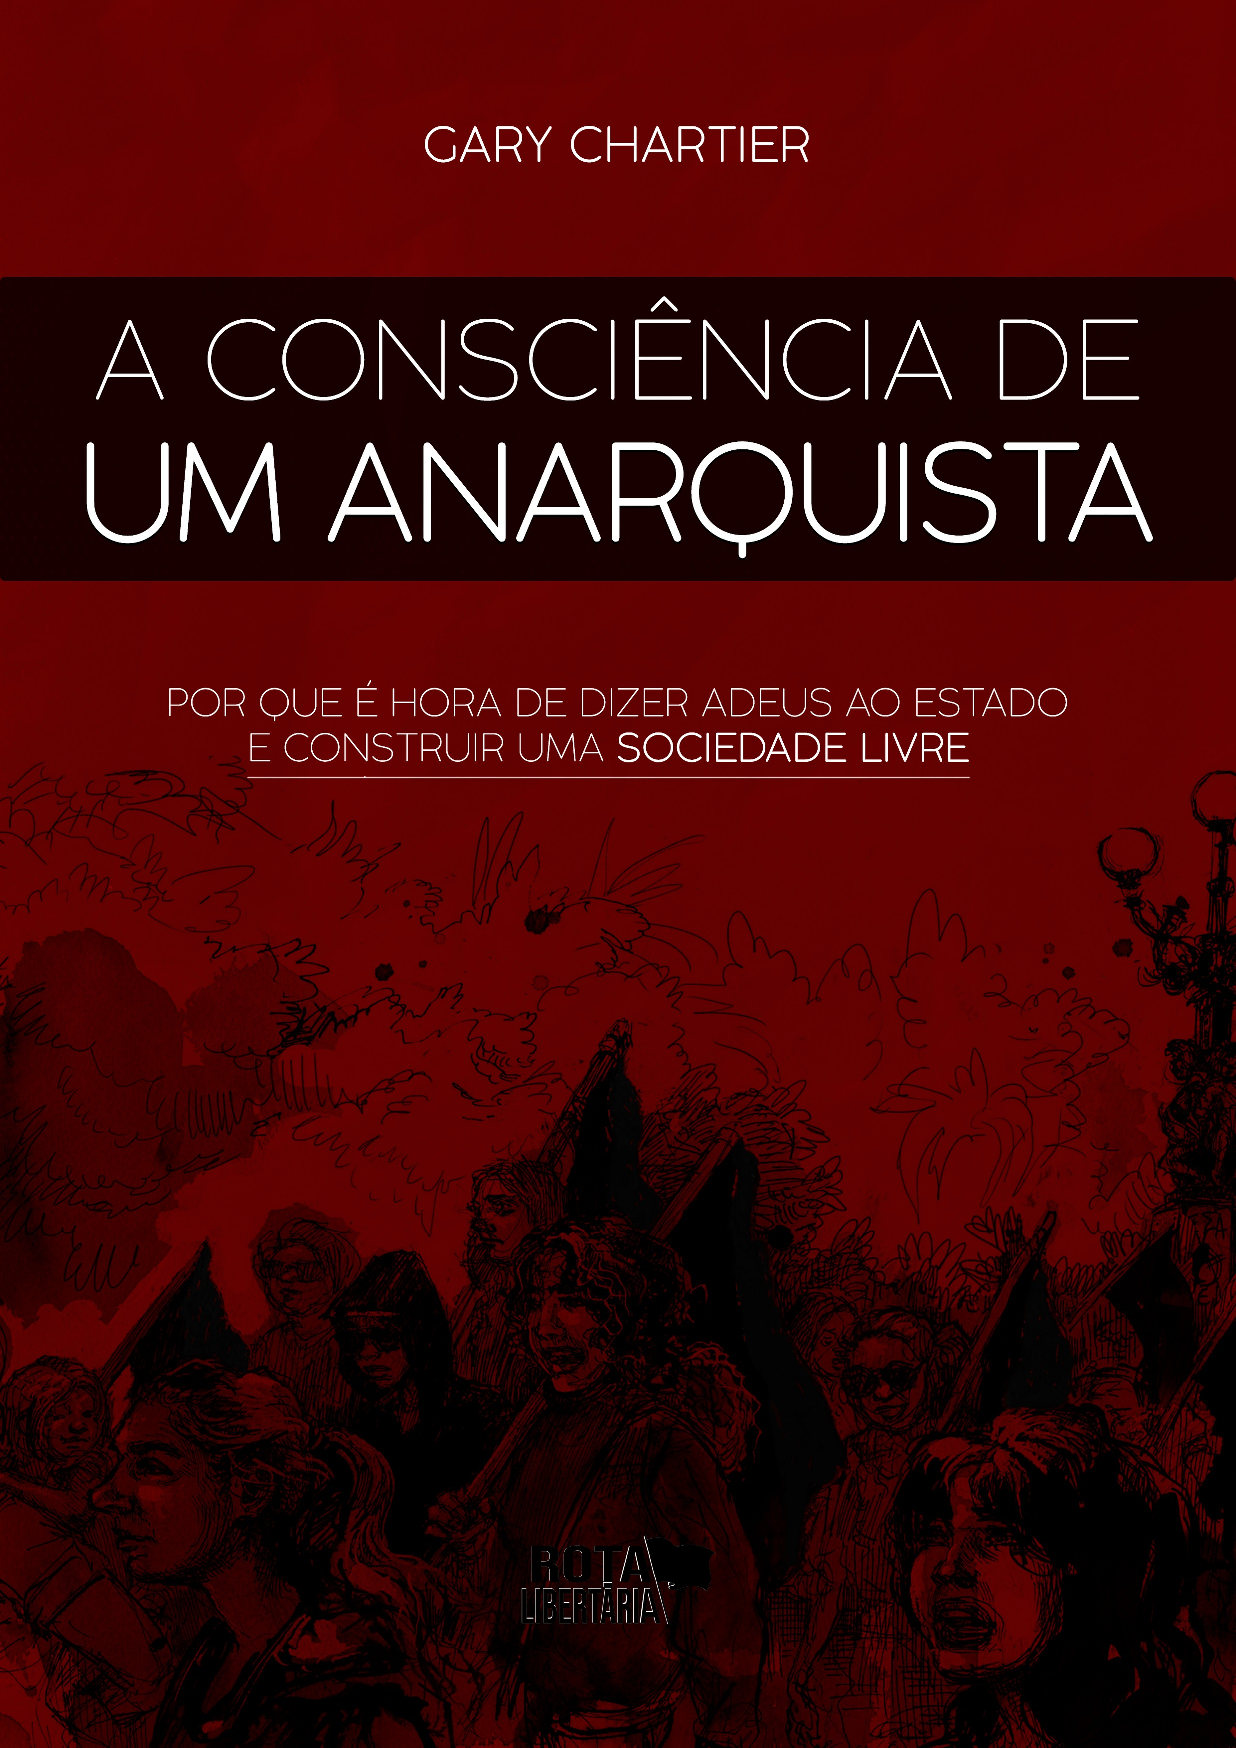
\includepdf{./assets/capa}

% Título

\newgeometry{bottom=3cm}

\begin{titlepage}
	\center	
	
	\vspace{30pt}
	
	\fontsize{14}{20}\selectfont\textsf{1ª Edição}
	
	\vspace{5pt}
	\fontsize{44}{52}\selectfont\textbf{A Consciência}
	
	\fontsize{26}{32}\selectfont\textbf{de um}
	
	\vspace{-28pt}
	\fontsize{56}{70}\selectfont\textbf{Anarquista}
	
	\vspace{10pt}
	\fontsize{20}{26}\selectfont\textsf{Por que é hora de dizer adeus ao estado\\e construir uma sociedade livre}
	
	%\raggedleft	
	
	%\vspace{12pt}
	%\fontsize{14}{20}\selectfont\textsf{1ª Edição}%\hspace{82pt}
	
	%\center
	
	\vfill
	
	\LARGE\textsc{Gary Chartier}
	
	\normalsize\emph{La Sierra University in Riverside, California} 
	 
	\vfill 
	        
	\normalsize Igor R.
	
	\small Tradução e Edição
	
	\vfill
	
	\vspace{5pt}
\end{titlepage}

\restoregeometry  

\begin{dedicatoria}
Para Elenor.
\end{dedicatoria}

\blankpage

\setcounter{tocdepth}{0} % ToC apenas com capítulos
\tableofcontents

\hypersetup{linkcolor=teal} % formata hyperref pós-ToC

% Nota do Tradutor

\chapter{Nota do Tradutor}

\lettrine[lines=2]{\textcolor{LettrineColor}{\textbf{T}}}{endo minhas convicções} sobre propriedade intelectual em mente, reservei um tempo para, sozinho, traduzir e editar o livro \emph{The Conscience of an Anarchist}, de Gary Chartier. O que quero dizer com isso é que essa é uma tradução livre, não oficial, de iniciativa própria, e que portanto não está diretamente associada nem a Gary Chartier, nem à \emph{Cobden Press}, nem ao \emph{Center for a Stateless Society}. Apesar disso, eu, como tradutor, mas acima de tudo como alguém apaixonado pelo anarquismo, gostaria de agradecer aos citados por toda energia dedicada à causa da libertação humana. Pois são esses esforços que, na forma de esperança, nos guiam em direção a um mundo mais significativo.

Como foi um empreendimento de uma pessoa só, é muito provável que essa tradução esteja repleta de erros. Ainda assim, dei o meu melhor para tornar esse projeto o mais profissional possível. Para isso, revisei a versão algumas vezes e adicionei notas de tradução (indicadas por ``N.T.'' e enumeradas em algarismo romano, ou então sinalizadas entre colchetes) para explicar expressões idiomáticas ou o que fosse necessário. Também dei muita importância para a edição do livro, que inclui uma capa feita pelo meu colega Eliãn -- agradeço a sua ajuda -- para o contentamento estético do leitor. Nesse quesito, acredito que o resultado tenha sido bem satisfatório.

\begin{flushright}
\large\emph{Igor R.}
\end{flushright}


\blankpage

% Agradecimentos

\chapter{Agradecimentos}

\lettrine[lines=2]{\textcolor{LettrineColor}{\textbf{E}}}{ste livro} reflete minha tentativa de reunir \emph{insights} que obtive desde que comecei a ler sobre anarquismo há mais de um quarto de século, \emph{insights} frequentemente obtidos como resultado de meus encontros com outros escritores. Baseei-me livremente nas ideias de uma variedade de pensadores anarquistas que argumentaram, de diferentes maneiras, a favor da superioridade da cooperação sobre a violência, da paz sobre a agressão, da liberdade sobre a coerção. Assim, embora eu tenha evitado referências específicas tanto quanto possível, anexei uma lista de \hyperref[chap:rec]{materiais} para o proveito de qualquer um que queira entender melhor o anarquismo.

Sou grato a diversas pessoas que dedicaram tempo e energia para ler e refletir sobre parte ou a totalidade deste livro durante o seu desenvolvimento: Kevin A. Carson, Brad Spangler, Teresa Warmke, Sheldon Richman, Thomas L. Knapp, Stephan Kinsella, D. Frank Robinson, James Tuttle e Gene Mayes. Jeff Riggenbach, David Henderson, Tom de Lorenzo, Pennelope Aletras-Leight e Armando Benitez editaram o manuscrito e me livraram de constrangimentos em diversos pontos. Eduardo Brugman, Esteban Salcido, Brandon Snider, A. Andrew Truong e Roderick T. Long, entre outros, contribuíram proveitosamente para o processo de \emph{design}. A assistência de Jim Person e de outros membros da equipe da \emph{Cobden Press} garantiu a produção e distribuição rápida de um livro atrativo e acessível. Estou muito satisfeito e grato pelo seu trabalho e sinto-me honrado em estar associado ao epônimo da \emph{Press}, Richard Cobden, cofundador da \emph{Anti-Corn Law League}, que desafiou os privilégios aristocráticos que limitavam o acesso das pessoas comuns a alimentos baratos, promoveu a causa da paz e da não intervenção, clamou por reduções nos gastos militares e rejeitou o mal da escravidão.

E agradeço, é claro, aos de sempre: Elenor Webb, Jeffrey Cassidy, Annette Bryson, Aena Prakash, Alexander Lian, Andrew Howe, Angela Keaton, Anne-Marie Pearson, Bart Willruth, Carole Pateman, Chelsea Krafve, Craig R. Kinzer, David B. Hoppe, David R. Larson, Deborah K. Dunn, Donna Carlson, Ellen Hubbell, Eva Pascal, Fritz Guy, Jan M. Holden, Jesse Leamon, Joel Sandefur, John Elder, John Thomas, Julio C. Muñoz, Kenneth A. Dickey, Lawrence T. Geraty, Ligia Radoias, Marc A. Benzakein, Maria Zlateva, Michael Orlando, Nabil Abu-Assal, Patricia Cabrera, Roger E. Rustad, Jr., Ronel Harvey, Ruth E. E. Burke, Sel J. Hwahng, W. Kent Rogers e Wonil Kim. Agradeço particularmente a Elenor pelo apoio moral e logístico e pelas acolhedoras oportunidades de diálogo e troca.

Pretendo doar todos os \emph{royalties} de autor recebidos com a venda desse livro para AntiWar.com. Sou imensamente grato pelas contínuas contribuições que aqueles associados a esse excepcional empreendimento jornalístico fazem a favor da causa da criação de uma sociedade organizada com base na cooperação pacífica e voluntária.

% Introdução

\chapter[Introdução]{Introdução\\\vspace{-1.75ex}\hrule\vspace{0.25ex}\normalfont\LARGE Abra sua mente para o anarquismo}

\lettrine[lines=2]{\textcolor{LettrineColor}{\textbf{C}}}{omo uma ideia}, o anarquismo é a convicção de que as pessoas podem e devem cooperar pacífica e voluntariamente. Como um programa político, é o projeto de agir sem o estado.

Dado que governos são fundamentados no uso da força, os anarquistas defendem que nenhum governo real é legítimo e que, de qualquer forma, estaríamos melhor sem o estado. Os anarquistas rejeitam qualquer tipo de autoridade adquirida ou mantida por meio de violência agressiva ou da fraude. De maneira mais ampla, muitos anarquistas -- incluindo eu -- defendem que os mesmos ideais que motivam sua oposição à violência agressiva os levam a contestar as instituições sociais e os padrões culturais que subordinam, excluem ou empobrecem as pessoas, complicam suas vidas, ou as forçam a uma conformidade que atordoa a alma.

As pessoas podem e devem organizar suas interações das suas próprias maneiras. Podemos nos defender contra agressões; não precisamos do estado para nos forçar a não matar uns aos outros. E não precisamos da ajuda do estado para coordenar as nossas interações. Trabalhando juntos, podemos construir vidas significativas e comunidades habitáveis.

\section{Anarquismo como visão positiva}

Às vezes, as pessoas usam o rótulo anarquista, ou hasteiam bandeiras pretas anarquistas, quando o seu principal objetivo é apenas o de espalhar o caos. Mesmo pessoas mais sensatas às vezes podem agir como se ``anarquia'' fosse apenas outra palavra para desordem. Mas o anarquismo como eu o entendo é sobre o melhor tipo de ordem que poderíamos imaginar: o tipo de ordem que surge voluntariamente, espontaneamente, à medida que as pessoas trabalham juntas de forma criativa para moldar suas vidas e planejar seus futuros. Anarquia é o que surge quando a ordem social se origina não dos canos das armas do estado, mas da cooperação pacífica e voluntária.

Grosso modo, um estado é uma organização que afirma ter autoridade legítima sobre quem usa a força em um determinado território e que faz um trabalho ao menos moderadamente eficaz de manter a violência não aprovada sob controle. (Mais sobre isso depois.) O estado no sentido moderno coexiste conosco a mais de trezentos anos, e estados dos mais variados tipos são muito mais antigos do que isso. Então é fácil assumir a existência dos estados como inevitável. Mas, para anarquistas, não há nada de necessário no estado. Os estados persistem por conta do interesse próprio de pessoas poderosas que os administram ou os manipulam e porque as pessoas comuns não perceberam o seu próprio poder de imaginar e implementar alternativas.

Neste livro, quero ajudar a afrouxar o controle que o estado ainda exerce sobre a imaginação das pessoas. Quero salientar que, como no famoso conto de Hans Christian Andersen, o imperador realmente não possui nada de especial. Quero encorajá-lo a mudar o seu ponto de vista -- a passar a ver o estado como um grupo de pessoas nem um pouco diferentes dos seus vizinhos, sem mais autoridade inerente, sem maior direito de dizê-lo o que fazer. (Claro, seus vizinhos provavelmente não irão ameaçá-lo com armas se você não fizer o que eles dizem. Mas essa diferença dificilmente se dá em favor ao estado.) Quero enfraquecer o mito de que o estado \emph{nos} representa em qualquer sentido significativo, de que, quando políticos e generais agem, eles estão agindo em \emph{nosso} nome. Quero enfatizar o fato de que as pessoas que tomam e executam as decisões estatais estão seguindo as suas próprias agendas, frequentemente em conflito com as nossas -- assim como as pessoas poderosas em grandes empresas e outras instituições semelhantes -- e que não temos razões para tratá-las com reverência, para vê-las como outra coisa senão \emph{pessoas comuns} com direitos \emph{exatamente como os nossos}.

Isso não é uma cartilha, um trabalho estritamente acadêmico sobre filosofia ou economia ou ciência política ou história, embora seja informado pelos resultados da investigação em todas essas disciplinas. É um \emph{manifesto}, um chamado para a ação: não para mais violência, que é apenas o reflexo da própria destrutividade do estado, mas para o empreendimento criativo de imaginar um novo tipo de sociedade e começar a construí-la aqui e agora, bem debaixo do nariz das pessoas no poder.

\section{Por que eu sou anarquista}

Eu sou anarquista por diversas razões.

Eu sou anarquista porque acredito que \emph{não existe direito natural de governar}. Acredito que as pessoas são iguais em dignidade e valor essencial, o que significa, por sua vez, que elas têm igual \emph{status} moral. Isso faz com que seja difícil justificar dar a algumas pessoas -- aqueles que governam o estado e aqueles que aplicam as decisões dos governantes -- direitos que outros não têm. E eu sou anarquista porque acredito que \emph{o estado não tem legitimidade}. Algumas pessoas argumentam que os governantes merecem ter mais direitos do que aqueles que eles governam porque seus sujeitos consentiram e continuam a consentir com a sua autoridade. Mas acredito que eles não o fazem. Falarei mais sobre essas razões para ser anarquista no \hyperref[chap:1]{Capítulo 1}.

Eu sou anarquista porque acredito que \emph{o estado é desnecessário}. Tento explicar o porquê no \hyperref[chap:2]{Capítulo 2}. Os estatistas costumam afirmar que ter um estado é a única maneira de ter uma sociedade pacífica. Eu discordo, tanto em bases teóricas quanto empíricas. Acredito que instituições não governamentais podem fornecer os serviços que o estado fornece -- mas de maneira mais eficiente e flexível; e há evidências sólidas de que elas são capazes de fazer isso. Além disso, tenho convicção de que se o estado tem o poder para fazer coisas boas, mesmo coisas muito boas, muito úteis, muito importantes, ele quase inevitavelmente usará esse poder de modo autoritário: ele usará o poder que possui para regular a vida das pessoas -- e para conseguir mais poder.

Como enfatizarei no \hyperref[chap:3]{Capítulo 3}, eu sou anarquista porque \emph{o estado vira a balança a favor das elites privilegiadas e contra as pessoas comuns.} (Ao contrário do que dirão as pessoas crentes nos ``bons governos'', isso é exatamente o que ele é projetado a fazer.) O estado tende a promover ineficiências através de subsídios, monopólios, patentes, tarifas e outros mecanismos que permitem que as elites se livrem de pagar os custos reais do que elas fazem. Ele força as pessoas comuns a arcarem com os custos das decisões da elite e a ajustarem as suas preferências e comportamentos para se adequar às maiorias conformistas. Acredito que uma sociedade sem estado teria mais chance do que a nossa de promover a eficiência e produtividade e evitar tipos de hierarquia e exclusão que os estados tendem a promover e proteger. Qualquer um que se preocupe com o poder dos ricos e das grandes empresas, a prosperidade das pessoas comuns e o bem-estar dos pobres e vulneráveis deve dizer um intenso ``não'' ao estado.

Eu sou anarquista porque \emph{o estado tende a ser destrutivo}. Ele se envolve em guerras e saques, e parece estar sistematicamente envolvido no aumento do nível de violência e injustiça para além das suas fronteiras -- que são, é claro, elas mesmas criações do estado (há mais sobre isso no \hyperref[chap:4]{Capítulo 4}). Acredito que uma sociedade sem estado apresentaria muito menos violência em larga escala do que a nossa.

Eu sou anarquista porque \emph{o estado restringe a liberdade individual} -- como uma forma de manter a ordem, beneficiar os privilegiados, preservar seu próprio poder ou subsidiar as preferências moralizantes de algumas pessoas. E há uma conexão natural entre o poder do estado e a imposição de restrições à liberdade. Apresento alguns exemplos no \hyperref[chap:5]{Capítulo 5}.

Eu sou anarquista porque desejo uma sociedade marcada pela diversidade, exploração e experimentação, porque acredito que os estados impõem a conformidade e resistem à criatividade e porque acredito que \emph{uma sociedade sem estado proporcionaria oportunidades para que as pessoas explorem diversas formas de viver vidas plenas e prósperas} e apresentem os resultados da sua exploração. Apresento esse ponto com mais detalhes no \hyperref[chap:6]{Capítulo 6}: falarei sobre a forma de vida sem o estado e delinearei alguns dos passos concretos que podemos dar para acabar com a opressão e violência e começar a criar um mundo novo.

\blankpage

\mainmatter

% Primeiro capítulo

\chapter{A Dissidência dos Governados}
\label{chap:1}

\lettrine[lines=2]{\textcolor{LettrineColor}{\textbf{E}}}{u sou anarquista porque} a reivindicação do estado à autoridade justificada é implausível. Ao contrário do que seus defensores afirmam, essa reivindicação não pode ser defendida com um apelo ao suposto consentimento daqueles que o estado procura governar.

Os Estados Unidos têm uma teoria política oficial. É uma teoria incorporada nas familiares palavras do segundo parágrafo da Declaração de Independência:\footnoteA{Estou focando neste e em outros exemplos americanos por diversas razões. Sou americano e conheço melhor o cenário americano. Acredito que a teoria política ``oficial'' dos Estados Unidos, conforme refletida na Declaração, e a atitude instintiva de muitos americanos em relação à autoridade do estado são especialmente receptivas ao anarquismo. E, ao mesmo tempo, ironicamente, abusos do poder americano dentro do país e no exterior destacam o quão perigosos os estados podem ser.}

\begin{quote}
Consideramos estas verdades como evidentes por si mesmas, que todos os homens são criados iguais, dotados pelo Criador de certos direitos inalienáveis, que entre estes estão a vida, a liberdade e a procura da felicidade. Que a fim de assegurar esses direitos, governos são instituídos entre os homens, derivando seus justos poderes do consentimento dos governados; que, sempre que qualquer forma de governo se torne destrutiva de tais fins, cabe ao povo o direito de alterá-la ou aboli-la e instituir novo governo, baseando-o em tais princípios e organizando-lhe os poderes pela forma que lhe pareça mais conveniente para realizar-lhe a segurança e a felicidade.
\end{quote}

Observe a frase central: os governos adquirem ``seus justos poderes do consentimento dos governados''. Acredito que isso aponta para a visão do poder estatal que muitos americanos automaticamente aceitariam. E há algo muito plausível nisso.

Afinal, as pessoas que formulam e implementam as decisões do governo são apenas isso -- pessoas. Se, como a Declaração também insiste, todas as pessoas são iguais em valor moral e direitos morais, então ninguém -- nenhum imperador ou rei ou príncipe, nenhum papa ou lama ou imame, mas também nenhum presidente ou senador ou governador -- tem um direito natural de governar. Como ninguém tem o direito natural de governar, qualquer reivindicação de governo é inerentemente suspeita. Então a igualdade moral básica das pessoas que a Declaração testifica cria uma presunção de anarquia. Se as pessoas são moralmente iguais, cabe à pessoa que afirma que alguém tem autoridade sobre os outros mostrar o porquê. De onde essa autoridade deveria vir? O que deveria fundamentá-la?

\section{Consentimento e autoridade}

A Declaração tem uma resposta para essa questão: uma autoridade governamental pode ter o direito de me governar \emph{se eu der a ela esse direito}. Ninguém é naturalmente um governante; mas, sugere a Declaração, alguém poderia adquirir a autoridade de um governante se o povo que esse alguém devesse governar \emph{consentir}.

Mas seria difícil apontar para qualquer estado existente cuja autoridade se firma no consentimento real dos governados. Você consentiu com a autoridade do estado em cujo território vive -- e comunicou seu consentimento às autoridades? Seus amigos o fizeram? Você conhece alguém que o fez? Não é surpreendente, acredito eu, que, em uma pesquisa de julho de 2010, 62\% dos americanos disseram que o governo dos EUA não tinha o consentimento dos governados, enquanto outros 15\% disseram que não tinham certeza. (Sete a cada dez dos pesquisados também relataram acreditar que o estado ``e as Grandes Empresas \ldots\ [estavam] no mesmo time'' aliados contra as pessoas comuns.)\footnoteA{``23\% Say U.S. Government Has the Consent of the Governed,'' \emph{Rasmussen Reports} (Rasmussen Reports, July 16, 2010) <\url{http://www.rasmussenreports.com/public_content/politics/general_politics/july_2010/23_say_u_s_government_has_the_consent_of_the_governed}> (July 16, 2010).}

\section{Votar como consentimento}

Algumas pessoas argumentarão, é claro, que você o fez exatamente ao votar. Mas você realmente colocou seu selo de aprovação no estado só porque optou por votar em suas eleições? Não é óbvio que você o tenha feito.

Suponha que você more em uma pequena cidade invadida por um grupo de bandidos. Os bandidos, podemos supor, são um bando ativo. Nem todos vão morar na \emph{sua} cidade; em vez disso, eles querem coletar tributo de várias comunidades vizinhas. Mas eles pretendem ocupar a sua vila para manter todos na linha. Para deixar clara sua benevolência -- e para ajudar a seduzir você e seus conterrâneos a apoiar o governo deles -- eles anunciam que você poderá escolher entre dois subordinados do chefe dos bandidos, Jean e Chris. Um deles governará a sua vila, mas você escolherá quem. Chris tem ataques de fúria, enquanto Jean tende a ser mais calmo e agradável. Então você e a maioria de seus companheiros da vila expressam seu apoio a Jean. Há alguma razão para pensar que, ao escolher Jean, você endossou a ocupação dos bandidos em sua vila? Dada uma escolha forçada, você selecionou a opção com maior probabilidade de beneficiar a vila, mas certamente fazer isso não é o mesmo que apoiar a presença dos bandidos.

Certamente o mesmo é verdade quando você decide se vai votar em uma eleição nacional, estadual ou local. Sua escolha de votar fornece uma boa evidência (se não uma evidência irrefutável) de que você prefere o candidato em quem votou em relação aos outros. Mas não fornece nenhuma razão particularmente boa para pensar que você deseja ser governado por um dos candidatos -- ou, na verdade, que deseja ser governado por alguém sequer.

\section{Imobilidade como consentimento}

De acordo com outro argumento estatista, simplesmente permanecer dentro do território de um estado de alguma forma constitui consentimento à sua autoridade. Mas não há nenhuma razão óbvia para isso. Certamente, permanecer no território reivindicado por um determinado estado não é interpretado de maneira mais natural como um sinal de apoio à autoridade do estado. Talvez eu permaneça lá porque as oportunidades de trabalho são abundantes, ou porque meus amigos estão lá, ou porque gosto do estilo da arquitetura. E talvez eu não me mude de lá porque gangues de bandidos parecem estar no comando de todos os outros lugares. Não é nada óbvio que ficar parado comunicaria a um observador razoável a mensagem de que provavelmente concordei com a autoridade do estado. O que exatamente na minha permanência deveria comunicar a mensagem de que aceito a autoridade do estado?

Bem, talvez o estado fixe sinalizações em todo o seu território com a seguinte frase: ``Quem permanecer por mais de vinte e quatro horas dentro do território mostrado nesta sinalização e marcado por várias placas de sinalização semelhantes, assim sinaliza consentimento à autoridade do Soberano Reino da Bozarkia.'' Se ele o fizer, e daí? Existem muitas razões, como sugeri, pelas quais as pessoas podem ficar exatamente onde estão que não seja por seu consentimento à autoridade de Bozarkia. Ficar parado não \emph{sinaliza} consentimento. Bozarkia precisa alegar que isso \emph{constitui} consentimento.

Os governantes da Bozarkia poderiam razoavelmente alegar que isso constituiria consentimento à sua autoridade somente se eles já \emph{tivessem} autoridade legítima sobre o território em que as sinalizações foram fixadas. Se esse fosse o caso, então, pelo menos em algumas circunstâncias, talvez eles pudessem legitimamente insistir que as pessoas deixassem o território. Nesse caso, as pessoas que permanecem podem estar agindo de má fé se escolherem permanecer em condições diferentes das estabelecidas pelos governantes de Bozarkia. (Mesmo então, se eles deixassem claro que não consentiram, e as autoridades bozarkianas os deixassem permanecer de qualquer maneira, o argumento das autoridades perderia muito da sua força.) Mas se a suposição é que um estado com autoridade sobre um determinado pedaço de território pode insistir que as pessoas ou façam o que ele diz ou deixem o território, há um problema bastante óbvio nesse caso: o que Bozarkia deveria estar tentando fazer nesse exemplo é \emph{estabelecer} a sua autoridade. Um procedimento para estabelecer a autoridade do estado que assume que o estado já \emph{possui} autoridade não demonstra muita coisa.

Os aspirantes a governantes da Bozarkia podem ter o direito de exigir obediência das pessoas já obrigadas a aceitar a sua autoridade; mas se eles possuem alguma autoridade ou não é exatamente o ponto em questão. É fácil imaginar que minha fixação de sinalizações afirme a minha autoridade e insista que as pessoas que permanecem em suas casas aceitam minha autoridade ao fazê-lo, em todo o bairro em que moro. Se as pessoas da vizinhança não conseguissem derrubá-las e não se mexessem, estariam elas aceitando minha autoridade como governante local? Certamente não, e elas claramente estariam em seus direitos ao simplesmente me ignorar. Isso é porque eu não tenho autoridade para insistir que elas aceitem meu governo ou deixem suas casas \emph{para início de conversa}.

A ideia de que permanecer no território de um estado equivale a consentir à sua autoridade não funciona. Permanecer não \emph{sinaliza} consentimento; fazê-lo comunica muitos significados possíveis. E permanecer equivale a \emph{aceitar} a autoridade do estado apenas se já tivermos estabelecido que o estado realmente \emph{possui} autoridade para início de conversa.

Há boas razões para pensar que muitas pessoas não consentiram com a autoridade do estado. Mas \emph{há} pessoas que apoiam a autoridade do estado e querem que o resto de nós se alinhe. Elas insistem que devemos obediência ao estado. Teriam elas algum argumento restante uma vez que mostramos que não consentimos à autoridade do estado (ou que nunca consentimos para início de conversa ou que retiramos nosso consentimento depois de perceber o desastre que o estado realmente é)?

\section{Consentimento como exigido para a justiça}

Estatistas podem ser engenhosos. Existem outros argumentos que eles podem oferecer para mostrar que o estado \emph{é} realmente legítimo. Por exemplo: ``Talvez você tenha retirado seu consentimento'', eles podem dizer. ``Talvez você nunca tenha consentido para início de conversa. Mas é injusto da sua parte \emph{não} consentir.''

Obviamente, há uma grande diferença entre ser obrigado a um acordo que eu realmente fiz e ser obrigado a um acordo que alguém pensa que eu \emph{deveria} ter feito. Mas ignore isso por enquanto. Por que seria injusto da minha parte desconsiderar as ordens do estado?

O estatista pode tentar explicar desta forma: ``A maioria decidiu que uma determinada demanda deve ser provida. Você é obrigado a colaborar, mesmo que discorde. Caso contrário, você estaria alegando que sua posição minoritária deve governar, e não a opinião da maioria.''

Como outros argumentos estatistas, esse não é muito bom. Claro, o anarquista \emph{não está} dizendo tal coisa: o anarquista não acredita que \emph{alguém} deva governar. E o argumento assume, novamente, exatamente o que deve provar. Se o estado realmente fosse um empreendimento cooperativo que todos nós tivéssemos escolhido participar, e se tivéssemos consentido com um conjunto de regras básicas, incluindo a regra da maioria, então seria injusto recusar essas regras apenas porque elas levaram a resultados que não gostamos. Mas a questão é precisamente se \emph{concordamos} com as regras básicas. Muitos de nós não o fizemos.

\section{Consentimento como exigido por aceitar benefícios}

Outro argumento estatista sugere que, se aceitamos benefícios do estado, nada mais justo que obedecê-lo. Mas esse argumento tenta provar demais.\footnoteNT{Nota do Tradutor [N.T.]: No original, \emph{prove entirely too much}. No contexto da filosofia, diz-se que um argumento ``\emph{proves too much}'' (ou, nesta tradução, ``prova demais'') quando ele também pode ser usado para provar uma proposição que o argumentador toma como falsa.}

Ele não fornece nenhum apoio para a obediência-ao-estado-em-geral, mas apenas para qualquer obediência que possa ser necessária para garantir a provisão de quaisquer benefícios que alguém venha a receber do estado. Suponha que eu gratuitamente aceite os serviços de saúde providos pelo estado, por exemplo. Talvez isso pudesse tornar injusto que eu evitasse contribuir para o sistema de saúde do estado. Mas não fornece nenhuma razão em específico para que eu coopere com o estado quando ele tenta impedir que outras pessoas leiam ou digam coisas que as autoridades não gostam ou quando ele me alista nas forças armadas.

O tipo de obediência envolvida aqui é claramente apenas o tipo de obediência envolvida em fornecer apoio financeiro para este ou aquele esquema patrocinado pelo estado. Mas a realidade é que não tenho nenhuma escolha significativa para fazer isso de tal forma. Se eu não obedecer quando o estado exige dinheiro de mim, tenho boas razões para temer que ele irá confiscar meus bens ou me prender. Uma vez que já estou sendo tributado de forma a apoiar uma variedade de serviços providos pelo estado -- tanto os que eu talvez queira que sejam providos, quanto os que eu definitivamente \emph{não} quero que sejam providos --, não há nenhuma razão para não tirar proveito dos benefícios relevantes. Mas isso dificilmente significa que estou consentindo com a operação do sistema em que minhas contribuições são tomadas de mim e dos outros.

Aceitar os benefícios providos pelo estado não significa que você está endossando o estado como um todo. Já que você está sendo forçado a pagar pelos programas que provêm esses benefícios, muitas vezes você nem irá se deparar com a questão de se seria \emph{justo} você não pagá-los, a não ser que você esteja disposto a enfrentar a prisão e a apropriação de seus bens pelo estado. E se você \emph{conseguir} evitar pagar o dinheiro que o estado deseja que você pague, não há do que você se sentir culpado desde que recuse os benefícios que ele oferece. Muitos anarquistas insistiriam que, enquanto uma organização (incluindo o estado) reivindicar tributos sob a mira de uma arma, ela não merece nada, mesmo pelos serviços que ela fornece. Mas mesmo que você deva algo em troca de serviços específicos que recebe voluntariamente, é difícil argumentar que você deve ao estado o pagamento por qualquer benefício que você \emph{não} aceite voluntariamente. E mesmo que você deva ao estado algum tipo de compensação por um benefício específico, aceitar esse benefício não o compromete a aceitar qualquer dever generalizado de \emph{obediência} ao estado.

Para turvar a questão ainda mais: mesmo que você \emph{aceite} benefícios providos pelo estado, e mesmo que deva algo em troca como resultado, ainda não está claro que você deve algo ao próprio \emph{estado}. Isso porque não foi \emph{realmente} o estado quem financiou os benefícios que você recebeu; e sim os pagadores de imposto comuns. Já que outros podem ser tributados com taxas mais altas porque você não paga pelos serviços que escolhe receber, você pode estar tratando \emph{eles} injustamente -- mas isso não significa que você tenha qualquer obrigação particular para com o próprio estado. Isso não torna legítimas as exigências do estado por tributos -- especialmente a reivindicação do estado da sua cooperação ou não interferência quando ele tenta fazer qualquer coisa \emph{além} de financiar quaisquer benefícios que você possa ter aceito de bom grado.

Suponha que os bandidos que mencionei anteriormente exijam uma certa quantia de tributo da sua cidade. Se for virtualmente garantido que mais será roubado dos outros porque você consegue evitar que os bandidos roubem de \emph{você}, pode haver circunstâncias em que os \emph{outros} teriam boas razões para vê-lo como tendo os sobrecarregado com fardos injustos. Mas você ainda não deveria nada \emph{aos bandidos em si}.

\section{Limites do consentimento}

É provável que não exista maneira de sinalizar consentimento à autoridade do estado. Afinal, pode-se esperar que o estado o puna -- tome suas coisas, o ataque fisicamente ou o prenda -- se você não obedecer as suas imposições. Então, só porque você coopera com os funcionários do estado, até mesmo se você declara publicamente o seu apoio ao estado, ninguém está realmente justificado a acreditar que você realmente consentiu livremente com a autoridade do estado. Ninguém pode legitimamente exigir de você uma promessa feita sob a mira de uma arma. Sempre corremos o risco de sermos colocados sob a mira de uma arma pelo estado. Então ninguém pode razoavelmente exigir de qualquer um de nós alguma promessa que deveríamos ter feito ao estado, já que qualquer promessa que poderíamos ter feito teria sido feita sob coação.

Além disso, se não houver uma maneira real de optar por \emph{sair} [\emph{opt out}], se o estado não fornecer uma maneira de permitir que as pessoas \emph{não consintam com sua autoridade} enquanto permanecem dentro do território que ele reivindica, então não há realmente nenhuma forma de optar por \emph{aceitar} [\emph{opt in}] também. O estado nos trata como se tivéssemos consentido com a sua autoridade em tudo que fazemos, então nem sequer estamos realmente tendo a escolha de consentir. E é difícil levar a sério a ideia de que seu consentimento \emph{significa} alguma coisa, que deve obrigá-lo de alguma forma, se você não tem a opção de não consentir.

\section{Apenas diga ``Não''}

Muitas pessoas, talvez a maioria delas, não consentiram deliberadamente com a autoridade do estado. E não há nenhuma razão geral para supor que a participação delas em várias atividades relacionadas ao estado ou a aceitação delas de vários benefícios relacionados ao estado as comprometa a consentir com isso. Na verdade, é bem possível que seja \emph{impossível} sinalizar consentimento à autoridade do estado de maneira confiável, dada a contínua ameaça de violência do estado contra as pessoas que não cooperam com as autoridades. Se a autoridade legítima depende do consentimento, parece que o estado provavelmente não é legítimo. E isso significa que você provavelmente não tem nenhum dever geral de obedecê-lo.

% Segundo capítulo

\chapter{Peixes, Bicicletas e o Estado}
\label{chap:2}

\lettrine[lines=2]{\textcolor{LettrineColor}{\textbf{E}}}{u sou anarquista porque} acredito que o estado não é nem necessário nem inevitável. Não precisamos do estado para prevenir a violência e preservar a ordem. O estado não é capaz de administrar a economia. E, apesar da pressão estatista, alternativas ao estado floresceram -- o que faz com que seja difícil ver o estado como inevitável.

\section{O estado como mantenedor da paz?}

Mesmo que ele não seja legítimo, dirão alguns estatistas, o estado é \emph{útil}. Apesar dele ser ilegítimo, realmente devemos apoiar a manutenção da autoridade do estado porque \emph{precisamos} dela. Precisamos dela, segundo o argumento, porque a ameaça de violência \emph{estatal} é necessária para nos proteger da violência de \emph{uns dos outros}. Se as pessoas souberem que o estado intervirá nos conflitos privados para manter a paz, teremos menos probabilidade de sermos roubados, assaltados e assassinados.

Para quem propõe esse tipo de argumento, a questão da legitimidade é irrelevante. Não importa se consentimos com a autoridade do estado ou não. Se não tivermos consentido, e daí? Consideração prudencial por nós mesmos e preocupação benevolente pelos outros estabelecem que mantenhamos o poder do estado. Caso contrário, nos encontraremos submersos em conflitos constantes, muitas vezes violentos.

É importante entender o que esse argumento \emph{não} estabelece. Ele não fornece nenhuma razão direta para que se preste atenção a qualquer comando decretado pelo estado. Ele \emph{apenas} fornece um argumento para apoiar a operação contínua do estado \emph{como um mecanismo para prevenir a violência} contra as pessoas ou seus bens. Se o estado opta por criminalizar alguma prática sexual que a maioria acontece de não gostar, por exemplo, ele está usando sua autoridade para reprimir a dissidência e impor a conformidade, e não, \emph{per se}, para inibir conflitos violentos. A menos que possa ser demonstrado que qualquer desacordo social corre um sério risco de se tornar uma disputa violenta e, portanto, requer ação preventiva por parte do estado, esse argumento sugere que o único tipo de estado que merece apoio é aquele que protege as pessoas contra a violência real -- um estado mínimo, de fato (e bastante diferente de qualquer estado que consigo imaginar no mundo atual ou em qualquer ponto da história do mundo).

\section{O quanto precisamos do estado?}

Mas por que deveríamos assumir, de qualquer forma, que precisamos do estado -- uma organização com o monopólio do uso da força em um determinado território -- para nos proteger contra a violência? 

Afinal, as pessoas podem se proteger contra a violência. Vizinhos podem vigiar as casas e locais de trabalho uns dos outros; eles podem trabalhar juntos para repelir quem é violento. E, mesmo sem o estado, o trabalho de algumas pessoas poderia ser o fornecimento de proteção contra a violência: o emprego de alguém poderia ser o de defender os outros de ataques violentos (e, talvez, de realizar tarefas relacionadas, como recuperar bens perdidos e obter reparações dos agressores). Não há nada logicamente contraditório ou praticamente impossível na entrega desses tipos de serviços por voluntários ou trabalhadores sem o envolvimento do estado. Por que a necessidade de serviços de proteção implicaria qualquer necessidade do estado?

Uma resposta comum é que, sem o estado, os mantenedores da paz, sejam eles voluntários ou profissionais, poderiam acabar envolvidos em conflito entre si. Assim, dizem os estatistas, uma estrutura abrangente é essencial para evitar conflitos violentos entre facções armadas.

À primeira vista, essa afirmação não parece totalmente plausível. Afinal, não existe um estado mundial supervisionando o comportamento de cada país. Mas a maioria deles não está em guerra na maior parte do tempo. Em vista dos custos da violência, e porque as pessoas são mais propensas a aderir a normas que exigem paz, uma autoridade abrangente com o monopólio da violência não parece obviamente necessária para impedir que atos agressivos ocorram.

Grupos individuais de vizinhos e trabalhadores terão semelhantes razões para evitar se envolver em violência. E, em uma pequena escala, no nível do bairro ou cidade, os custos da agressão serão ainda maiores: será mais fácil que comunidades mantenham normas anti-agressivas e que vizinhos que desaprovam o comportamento agressivo dos outros os penalizem por suas ações pouco razoáveis. E, é claro, os custos e problemas de coordenação envolvidos quando um bairro tenta se defender contra bandidos de outro bairro serão muito mais administráveis do que aqueles envolvidos quando um estado, com fundos originados de impostos à sua disposição, entra em guerra com outro estado.

Um estado, por definição, exerce o poder de monopólio. E monopolistas são notoriamente ineficientes. Quando uma empresa pode impedir legalmente que qualquer outra faça o mesmo trabalho que ela realiza, ela cobrará preços exorbitantes e fornecerá um serviço ruim. Nossa experiência com outros monopolistas certamente não nos dá nenhuma razão para pensar que o estado, um monopólio, provavelmente fornecerá segurança, justiça e outros serviços de alta qualidade a baixo custo. E, claro, o estado está sob ainda menos pressão para fornecer serviços de alta qualidade e baixo custo do que um monopolista comum: um monopolista comum pode excluir outros de fornecer os bens e serviços que ele oferece, mas as pessoas geralmente são livres para evitar a compra desses bens e serviços; em contraste, o monopólio que o estado é pode e de fato força as pessoas a comprarem o que ele vende, nas condições que ele mesmo estabelece.

Ainda mais problemático é o fato de que o estado é uma entidade extremamente \emph{perigosa}. Ele é frequentemente violento -- em larga escala. Embora os estados de fato controlem o mau comportamento de gangues menores de criminosos, eles frequentemente oprimem seu próprio povo e atacam e espoliam o povo de outros estados. Não existe em última análise uma maneira significativa de agregar e comparar diferentes atos de violência. Mas parece claro que as mesmas razões gerais que podemos ter para temer atos violentos cometidos por outras pessoas são razões para temer o mau comportamento do estado.

Os custos diretos e indiretos da violência são consideráveis e não quero subestimá-los. Esses custos estão certamente entre as importantes razões pelas quais uma sociedade sem estado não teria de ser destruída pela violência entre facções armadas. Mas não há razão alguma para pensar que a maioria das pessoas, na maioria das sociedades hoje, são pacíficas e cooperativas principalmente porque temem que o estado retaliará com violência se elas se comportarem de maneira agressiva. A maioria das pessoas, suspeito eu, respeitam as normas sociais que exigem interações pacíficas e voluntárias com outras pessoas por outras razões. Elas conseguem compreender a razoabilidade dessas normas, tanto do ponto de vista moral quanto prático (precisamos uns dos outros, afinal, e paz e cooperação geralmente são mais agradáveis do que violência). E essas normas foram incutidas nessas pessoas por ensinos e modelos, tanto deliberados quanto inconscientes. E poderia-se razoavelmente esperar que o mesmo tipo de ensinos e modelos desempenhariam o papel que já desempenham hoje em uma sociedade sem estado.

\section{Paz interna, guerra externa}

Consigo imaginar que um estatista possa argumentar, em resposta ao que eu disse, que há consideravelmente menos violência dentro de um determinado país do que entre países (não tenho certeza se concordo com isso, mas aceitarei para fins de argumentação) porque dentro de um país existe um sistema de legislação e resolução de disputas que foi acordado.

O estatista pode dizer algo assim: não importa se existe uma única agência policial dentro de um estado: muitas vezes, na verdade, existem muitas dessas tais agências, muitas vezes administradas e financiadas de forma independente. O que importa, ao invés disso, é que haja um acordo geral sobre os princípios jurídicos que essas agências devam seguir e sobre os tribunais cujas decisões elas devam aplicar. É esse acordo, o estatista pode argumentar, que garante que diversas agências de aplicação da lei possam cooperar para manter a paz dentro de um estado.

Observe que, a esse ponto, o estatista fez uma enorme concessão ao anarquista. O estatista reconheceu que uma única agência absolutamente poderosa não é necessária para manter a paz. Considere os Estados Unidos: não há base plausível para sustentar que todas as agências nacionais, estaduais e locais de aplicação da lei formem um único empreendimento cooperativo, uma organização gigante e coordenada. Essas agências certamente influenciam umas às outras. Claramente existem pessoas que gostariam de centralizar o controle das agências de aplicação da lei, e temos toda razão para temer o tipo de poder que poderia ser exercido sobre as pessoas comuns se elas \emph{fossem} centralizadas. Mas hoje em dia, elas são obviamente independentes, e o estatista não parece inclinado a disputar isso: ele está reconhecendo que muitas diferentes agências de aplicação da lei podem coexistir pacificamente. No entanto, defende ele, sua coexistência pacífica depende do reconhecimento mútuo da autoridade do sistema jurídico.

O estatista, no entanto, não deveria dar muita importância a esse fato. Afinal, existem muitos sistemas jurídicos diferentes. Os policiais em Louisiana não aplicam e obedecem às mesmas leis estaduais e decretos locais que suas contrapartes em Massachusetts, nem respondem aos mesmos tribunais. Uma considerável diversidade jurídica é claramente compatível com a paz social. E está claro que as pessoas podem resolver disputas pacificamente apesar dos conflitos entre sistemas jurídicos: tribunais podem aplicar regras de conflito de leis\footnoteNT{N.T.: \emph{conflict-of-law rules}. No contexto de regras do direito internacional, que mediam disputas envolvendo jurisdições diferentes.} para garantir que um processo razoável seja seguido e um resultado razoável alcançado quando alguém de Wyoming processa alguém de Missouri por uma disputa que diz respeito a um evento na Califórnia, mas que está, por acordo, sujeito às leis de Delaware. (Na verdade, regras de conflito de leis tornam possível a resolução metódica de disputas envolvendo sujeitos e sistemas jurídicos de diferentes \emph{estados}.)

O estatista talvez concorde que é possível haver disputas metódicas entre pessoas que se identificam com comunidades cujos sistemas jurídicos diferem. Mas ele pode optar por manter uma posição recuada: no mundo de hoje, estados e governos locais reivindicam autoridade absoluta sobre as pessoas que vivem em seus respectivos territórios; as pessoas podem confiar que aqueles supostamente sujeitos a outros sistemas jurídicos manterão seus acordos porque seus governos os obrigarão a fazê-lo. Mas ninguém obriga agentes governamentais a exigir que as pessoas cumpram seus acordos. Eles cooperam uns com os outros, suspeito eu, como resultado de uma combinação de fatores: normas que ditam justiça e cooperação, o desejo de reputações que levem à contínua confiança e cooperação e os custos dos conflitos que poderiam surgir caso eles encorajassem as pessoas a ignorar suas obrigações. Os mesmos tipos de fatores incentivariam as pessoas em uma sociedade sem estado a cooperar umas com as outras; eles também alinhariam as pessoas que tomam decisões, influenciando instituições das várias comunidades em tal sociedade, de forma a favorecer a cooperação em vez da negligência para com as obrigações.

O exemplo local que o estatista deseja invocar aqui de fato parece depender principalmente de um consenso sobre regras de escolha da lei aplicável\footnoteNT{N.T.: \emph{choice-of-law rules}. No mesmo contexto da nota de tradução anterior.}, uma vez que, obviamente, não depende da existência de um único corpo de legislação relevante ou de uma única agência de aplicação da lei. E regras de escolha da lei aplicável podem obviamente ser utilizadas para resolver disputas em uma sociedade sem estado da mesma forma que em um estado moderno com diversos sistemas jurídicos. 

Talvez o estatista queira dizer que, embora existam diversos tipos de agências de aplicação da lei e sistemas jurídicos nos Estados Unidos, por exemplo, a polícia nacional e agências militares estão sempre disponíveis para resolver conflitos entre eles. Segundo essa visão, a capacidade de coexistência dos diversos sistemas jurídicos depende da disponibilidade da violência do estado em segundo plano como meio de regular disputas. Sem a ameaça da força pelas agências nacionais, conflitos entre as agências locais de aplicação da lei seriam tão frequentes quanto conflitos entre exércitos nacionais.

No entanto, não tenho certeza se o monopólio da violência do estado é realmente o único fator relevante aqui. Primeiro, em alguns estados a violência é comum. A vida de muitas pessoas em muitos estados é violenta e, bom, bastante ruim. Estados nem sempre mantêm a violência sob controle. E estados frequentemente se envolvem em violência contínua contra pessoas que vivem dentro de ``suas'' fronteiras. Então não está claro se uma comparação entre violência intraestadual e violência interestadual sempre resulta a favor do estado. Em segundo lugar, o nível de violência dentro de um determinado estado que não resulta dos crimes do próprio estado não é apenas consequência do grau em que o estado ameaça usar a força contra indivíduos violentos. Pobreza, laços econômicos, normas culturais e homogeneidade cultural (ou a existência ou a não existência de normas culturais que promovem respostas bem-sucedidas à heterogeneidade cultural) também importam. Não é muito surpreendente que o nível de violência na maioria das sociedades ocidentais seja relativamente baixo. Mas o baixo nível de violência provavelmente é consequência do fato de que essas sociedades são economicamente confortáveis, que as pessoas são economicamente interdependentes e que os valores que apoiam a cooperação e a paz social são amplamente difundidos. Todos esses fatores parecem estar presentes nessas sociedades, quer exista estado ou não. Então a relativa estabilidade dessas sociedades não fornece evidências particularmente fortes para a importância da autoridade do estado.

Normas que favorecem a cooperação e a justiça e se opõem à força agressiva provavelmente tenderiam a manter as coisas relativamente calmas mesmo sem a ameaça de violência do estado. Além disso, os custos de atacar os outros seriam consideráveis -- e, sem o estado, seriam arcados (dependendo de como uma determinada comunidade organizou os serviços de segurança) por voluntários, membros de cooperativas de defesa mútua, instituições de caridade ou trabalhadores no ramo da segurança e defesa em tempo integral e aqueles que os pagam. É provável que nenhuma dessas pessoas ficariam muito felizes em arcar com os custos financeiros associados a conflitos violentos, custos que incluem tempo desperdiçado, recursos perdidos, reputação manchada, danos físicos e morte. E isso significa que haverá considerável pressão para evitar esse tipo de conflito, de fazer acordos com outras pessoas que tendem a reduzí-los e de evitar pessoas que tendem a provocá-los.

Eu falei aqui sobre comunidades e, para simplificar, tratei uma comunidade como geograficamente localizada. Mas ela certamente não precisa ser assim. As pessoas podem pertencer a diversas comunidades sobrepostas. E diferentes comunidades -- diferentes redes e organizações socais, congregações religiosas, clubes, grupos de pessoas envolvidas no mesmo tipo de trabalho -- podem perfeitamente manter diferentes sistemas jurídicos. Diferentes tipos de grupos podem desenvolver corpos jurídicos apropriados para diferentes tipos de circunstância e diferentes tipos de disputa. E onde as preocupações de grupos diferentes se sobrepõem, os mesmos tipos de regra de conflito de leis que regem as disputas entre pessoas de comunidades territorialmente distintas podem ser aplicadas.

\section{Um tipo diferente de governança}

Lembre-se das palavras da Declaração. Seus signatários insistiram ``que, sempre que qualquer forma de governo se torne destrutiva de tais fins, cabe ao povo o direito de alterá-la ou aboli-la e instituir novo governo''. Mas e se nenhum estado sequer receber (ou merecer) o consentimento do povo? Os diversos e imprevisíveis mecanismos de resolução de disputas que se desenvolverão em uma sociedade sem estado podem ser origens confiáveis de ordem e segurança. Substituir o estado pelo tipo de anarquia que estou falando aqui não é uma questão de eliminar o governo se ``governo'' realmente significa apenas ``governança'' -- gestão, administração, criação e manutenção da ordem. Criar uma sociedade sem estado significa criar um tipo particular de gestão, administração, manutenção da ordem -- um tipo que não depende da violência, da posse de ninguém do monopólio da força.

A paz é produtiva; a violência é custosa. Laços comunitários unem pessoas umas às outras e reforçam as normas de cooperação, justiça e compaixão. E à medida que comunidades humanas exploram e experimentam, elas podem conceber uma enorme variedade de estratégias criativas para a resolução de conflitos sem o monopólio da força do estado. Ao contrário do argumento estatista de que não teríamos paz sem o estado, as pessoas que querem paz precisam menos do estado do que um peixe precisa de uma bicicleta (a bicicleta, afinal, dificilmente fará mal ao peixe, enquanto o estado é positivamente perigoso).

\section{O estado e a economia}

O argumento mais comum a favor do estado nos dias de hoje é provavelmente a afirmação de que ele é necessário para prevenir a violência. Acredito que esteja claro que esse argumento não funciona, que diversos meios de preservar e restaurar a paz estariam disponíveis em uma sociedade sem estado. Outro argumento de que o estado é indispensável pode ser de que as pessoas precisem do estado porque uma autoridade central é necessária para guiar a produção e distribuição de bens e serviços. Mas também não acredito que o estado seja necessário para administrar a produção e a distribuição de maneira eficiente -- na verdade, quase certamente ele \emph{não pode} fazê-lo.

Existem várias razões interrelacionadas para isso. Acredito que a mais essencial é que o estado não sabe realmente o que as pessoas querem ou quais recursos estão disponíveis. Ele sem dúvidas poderia reunir um vasto banco de dados de todos os recursos físicos, trabalhadores e suas habilidades disponíveis. Mas nada como isso existe hoje em dia; seria extremamente caro e demorado; exigiria a implementação de um poder computacional quase inimaginável; e apenas ter as informações necessárias sem dúvida daria aos agentes estatais uma capacidade tremenda de manipular a vida das pessoas.

Mas suponhamos que todos esses obstáculos possam ser superados. Ainda seria o caso que o estado não teria conhecimento das preferências reais das pessoas por bens e serviços. Não, não há dúvidas de que ele poderia simplesmente administrar a produção e distribuição sem considerar as preferências das pessoas, apenas decidindo o que elas precisam e entregando os bens e serviços que ele decidiu produzir como resultado. Mas alguém realmente acredita que isso seria sensato? As pessoas sabem muito mais sobre suas próprias circunstâncias e, portanto sobre o que seria útil ou não para elas, do que burocratas do estado. E, claro, apenas desfrutar da liberdade de escolher qual dos diversos bens se deseja é importante por si só.

Talvez o estado pudesse fazer uma pesquisa com as pessoas para determinar as suas preferências. Ele poderia até mesmo manter registros de pesquisas individuais para que soubesse exatamente o que cada indivíduo deseja. Mas, novamente, isso daria ao estado um poder enorme. Isso exigiria um imenso investimento em gerenciamento de dados. E exigiria que as pessoas dedicassem um bom tempo respondendo às perguntas da pesquisa.

Imagine que esse conjunto de problemas pudesse ser resolvido. Ainda assim não resolveria a dificuldade associada a recursos finitos: nem todas as coisas que desejo são coisas que posso ter; tenho que fazer escolhas; tenho que racionar recursos escassos. Para determinar como realizar essa tarefa, o estado teria que pedir às pessoas não apenas para fornecer preferências, mas para pesá-las em relação umas às outras, para haver uma ideia de quanto tempo e energia devem ser gastos na entrega de quais bens e serviços em específico.

Para complicar ainda mais as coisas para o estado, nem sempre é óbvio quais informações são relevantes para o processo de planejamento da produção e distribuição de determinados bens. O estado pode não saber se deve ou não adquirir as informações de determinadas pessoas, e essas próprias pessoas podem não perceber que certas informações que possuíam eram relevantes.

Além disso, é extremamente improvável que o estado saiba com antecedência a maneira mais eficiente de resolver um problema específico de produção ou distribuição. O estado poderia direcionar investimentos a uma gama específica de abordagens -- mas ainda assim correria um risco significativo de ignorar alternativas que poderiam ser identificadas pelos outros de maneira criativa. Se, no entanto, ele apoiasse diversos empreendimentos de diferentes pessoas para identificar mecanismos criativos de produção ou distribuição, ele não saberia de antemão quais merecem apoio e, os que merecem, o quanto. É difícil imaginar que um sistema dirigido pelo estado não sufocaria a criatividade e ignoraria possibilidades inovadoras. 

Esse ponto é especialmente evidente se você pensar sobre a questão, não, \emph{Quantos widgets devemos fazer?}, mas sim, \emph{Devemos fazer widgets ou zidgets}? ou, de maneira ainda mais essencial, \emph{Devemos fazer uma fábrica que possa ser usada para construir peças para máquinas de fazer widgets (e muitas outras coisas), ou um tipo completamente diferente de fábrica}? Sob qual possível base o estado deveria tomar essas decisões? Que informação sobre as possíveis preferências do consumidor pode-se pensar que ele tem? Como recursos seriam racionados entre esses tipos de usos básicos? Suponha que o estado administre a economia determinando o nível de investimento em fábricas, terras comerciais e industriais, infraestrutura e assim por diante. Ele não pode perguntar sobre as \emph{preferências} do consumidor nesses casos e procurar condizer os níveis de investimento a essas preferências. Isso porque o próprio estado \emph{é} o consumidor -- ele será o comprador das terras e das fábricas -- e o que ele está tentando fazer é descobrir quais exatamente suas preferências deveriam \emph{ser}.

Existem razões gerais para pensar que a gestão eficiente da produção e distribuição de bens e serviços pelo estado (ou, de fato, por qualquer autoridade centralizada) não funcionaria. E essas razões se aplicam a quaisquer bens e serviços que eles realmente \emph{sejam}. Isso inclui a produção e distribuição de bens e serviços que os defensores do estado tipicamente querem sugerir que somente ele pode fornecer, aqueles que nossa necessidade supostamente ajuda a justificar o estado, mesmo que ele seja ilegítimo. O argumento, lembre-se, é de que precisamos do estado para evitar que matemos uns aos outros e para resolver conflitos. Mas não há nenhuma razão especial para pensar que o estado seria melhor em gerenciar centralizadamente a produção e distribuição econômica de serviços de prevenção da violência e resolução de conflitos do que em gerenciar centralizadamente a produção e distribuição econômica de outros bens e serviços. A inadequação do estado como gestor econômico ajuda a enfraquecer um argumento crucial frequentemente oferecido a favor de sua continuada existência.

Há também outro problema muito real relacionado à gestão estatal da produção e distribuição. O poder exigido para implementar tal sistema seria enorme. A tentação oferecida ao tirano em potencial pela disponibilidade de tal poder seria grande. E possuir esse tipo de poder possibilitaria que até mesmo burocratas bem-intencionados que cometessem erros causassem um enorme dano em pouco tempo.

O fato de que o estado não consegue administrar com sucesso a produção e distribuição econômica de bens e serviços não \emph{prova} que não deveria haver estado. Talvez, por exemplo, existam bens e serviços para os quais há boas razões que as pessoas desejem, mas que não podem ser produzidos economicamente. É por isso que meu argumento contra o estado é dividido em várias partes. Eu acredito, de fato, que é possível produzir todos os bens e serviços que poderíamos desejar sem o estado. Mas mesmo que se pudesse ser demonstrado que esse não é o caso, os outros tipos de razões que enfatizei, incluindo a ilegitimidade e a periculosidade essencial do estado, pesariam muito contra o estado. Acredito que faria sentido abandonar o estado mesmo que isso também significasse abandonar algumas outras coisas que poderíamos genuinamente desejar.

Os custos diretos de operação de um sistema estatal de gestão econômica seriam enormes. E existiriam diversos custos indiretos. Isso incluiria a produtividade reduzida resultante de qualquer tentativa de administrar o processo criativo de maneira centralizada. Também incluiriam diversos outros tipos de problemas -- evidentes nos dias de hoje mesmo em economias que não são totalmente administradas pelo estado. Estes incluem ineficiências criadas por subsídios estatais para elites privilegiadas, encargos impostos pelo estado sobre os pobres e incentivos fornecidos pelo estado que sustentam grandes organizações empresariais centralizadas -- incentivos que estimulam atividades econômicas ineficientes e sustentam organizações nas quais frequentemente é debilitante, alienante e opressivo trabalhar.

\section{A praticidade da anarquia}

Obviamente, resistir ao desenvolvimento de sociedades sem estado é muito do interesse das pessoas que supervisionam e lucram com as operações dos estados. O estado é tão claramente custoso e opressor que muitas pessoas provavelmente explorariam alternativas a ele com bastante entusiasmo se imaginassem que ele poderia ser substituído. O argumento mais prático a favor do apoio ao estado é que realmente não há alternativa à sua continuada existência. Apontei algumas razões gerais do porquê pode fazer sentido ser cético sobre essa afirmação. Mas o anarquista não precisa depender somente de argumentos abstratos sobre o que poderia funcionar ou o que provavelmente funcionaria. Em uma variedade de contextos, as pessoas parecem progredir com sucesso sem muita ou nenhuma ajuda de uma autoridade com o monopólio da força.

\subsection*{Relações entre estados}

Comece com o óbvio: não existe um estado mundial. Alguns estados são muito mais poderosos que outros, mas nenhum estado exerce ou reivindica algo parecido com o monopólio da força em todo o mundo (mesmo que alguns sem dúvidas gostariam de fazê-lo). É claro, existem conflitos. Mas na maior parte do tempo os estados interagem pacificamente. Eles resolvem disputas. Eles reconhecem a legitimidade dos resultados dos processos de resolução de disputas. E não há nenhum Big Brother pronto para obrigá-los a fazer isso. É justo apostar que eles fazem isso por diversos motivos: a violência é custosa; reputações são importantes de se manter; e sem dúvidas, pelo menos às vezes, os funcionários do estado realmente querem cooperar com os outros e realmente internalizaram normas que exigem um comportamento justo, respeitoso e pacífico. Qualquer que seja a explicação em qualquer caso particular, entretanto, os estados interagem sem o auxílio de um Leviatã mundial.

\subsection*{Comércio internacional}

E quanto às pessoas e organizações envolvidas na troca de bens e serviços além das fronteiras estatais? Sem um Leviatã global, não há ninguém para criar ou implementar qualquer tipo de lei comercial global. Certamente, existem tratados (embora, novamente, não haja nenhum estado mundial para fazer os estados aderirem a eles). Mas os tratados dificilmente cobrem todas as questões que podem surgir nas transações comerciais. Às vezes, árbitros resolvem disputas comerciais internacionais. Às vezes, tribunais nacionais os resolvem -- mesmo que fazê-lo signifique ter que interpretar e aplicar leis estrangeiras desconhecidas. Pessoas que são membros de diferentes comunidades políticas com diferentes sistemas jurídicos conseguem resolver disputas jurídicas sem depender de uma única autoridade abrangente com um monopólio da força e, às vezes, de fato, com a ajuda de mecanismos voluntários de arbitragem. O fato de que as disputas comerciais internacionais podem ser resolvidas sem a ajuda do Leviatã sugere que o estado é menos essencial do que as pessoas costumam supor.\footnoteA{Peter T. Leeson, ``One More Time with Feeling: The Law Merchant, Arbitration, and International Trade,'' \emph{Indian Journal of Economics and Business} spec. iss. (Sep. 2007): 29-34.}

\subsection*{A resolução autônoma de disputas dos comerciantes}

As pessoas também podem optar por sair do sistema jurídico do estado quando elas lidam umas com as outras \emph{dentro} das fronteiras do estado. Muitas pessoas fizeram isso por séculos durante a Idade Média e o Renascimento. A \emph{lex mercatoria}, a lei dos próprios comerciantes, surgiu como uma resposta previsível à ausência de padrões uniformes para transações comerciais envolvendo comerciantes de diferentes regiões. Comerciantes em viagem poderiam tirar proveito dos tribunais mercantis estabelecidos em feiras comerciais em toda a Europa. Os tribunais impunham padrões aceitáveis à comunidade mercantil -- bem razoáveis, uma vez que os padrões se aplicavam a disputas entre os próprios comerciantes. Os padrões foram aqueles que tinham evoluído ao longo do tempo à medida que comerciantes descobriam o que funcionava e o que não funcionava, o que era justo e o que não era, dados os tipos de circunstâncias em que eles caracteristicamente se encontravam. E mecanismos eficazes de aplicação muitas vezes incluíam boicotes dirigidos àqueles que se recusavam a pagar ou então a aceitar os julgamentos dos tribunais mercantis.

Sem dúvidas, os tribunais eclesiais e estatais também se envolveram em disputas comerciais, e boicotes dificilmente eram os únicos mecanismos de aplicação de leis. E não é como se houvesse um único código mercantil uniforme, escrito em tipo frio com seções enumeradas, aceito por todos comerciantes: havia, sem dúvidas, variações locais, e a lei local certamente tinha papel importante nessa ocasião. Com todas essas qualificações, no entanto,\footnoteA{Veja, por exemplo, Paul Milgrom, Douglass North e Barry Weingast, ``The Role of Institutions in the Revival of Trade: The Law Merchant, Private Judges, and the Champaigne Fairs,'' \emph{Economics and Politics} 2.1 (March 1990):1-23. Mas cp. Stephen Edward Sachs, ``From St. Ives to Cyberspace: The Modern Distortion of the Medieval `Law Merchant,'\,'' \emph{American University International Law Review} 21.5 (2006): 685-812. Focando na feira de St. Ives (registros de tribunal relacionados os quais ele examina detalhadamente), Sachs critica as afirmações de que a \emph{lex mercatoria} era uniforme, que as disputas dos comerciantes eram resolvidas principalmente pelas próprias instituições dos comerciantes e que autoridades locais não estavam envolvidas na resolução de tais disputas.} parece que os comerciantes medievais frequentemente conseguiam desenvolver e aplicar normas legais de maneiras que os ajudavam a resolver disputas envolvendo pessoas de diferentes jurisdições por conta própria, sem a participação do estado. Gerações posteriores de comerciantes continuaram a fazê-lo.\footnoteA{Veja, por exemplo, Lisa Bernstein, ``Opting out of the Legal System: Extralegal Contractual Relations in the Diamond Industry,'' \emph{Journal of Legal Studies} 21.1 (Jan. 1992): 145-53; Edward P. Stringham, ``The Extralegal Development of Securities Trading in Seventeenth Century Amsterdam,'' \emph{Quarterly Review of Economics and Finance} 43.2 (Sum. 2003): 321-44.} A experiência deles também levanta questões óbvias sobre a suposta indispensabilidade do estado como uma fonte de regras legais e de aplicação da lei.

\subsection*{Islândia medieval}

A Islândia medieval não era um paraíso anarquista. Mas funcionou razoavelmente bem sem instituições estatais para a administração da justiça e a manutenção da paz civil.\footnoteA{David D. Friedman, ``Private Creation and Enforcement of Law: A Historical Case,'' \emph{Journal of Legal Studies} 8.3 (Mar. 1979): 399-415; cp. William Ian Miller, \emph{Bloodtaking and Peacemaking: Feud, Law and Society in Saga Iceland} (Chicago: U of Chicago P 1997).} Nenhuma entidade detinha o monopólio do uso da força. Além dos fundos necessários para sustentar um único trabalhador em meio período, o sistema legal não dependia de qualquer tipo de receita tributária. Havia uma aceitação geral de um conjunto de normas que governavam a maneira que as instituições limitadas -- júris, assim como outros grupos, organizados mas basicamente voluntários, que arcavam com os custos de acesso dos membros aos tribunais -- atendiam às necessidades das pessoas. As instituições eram suficientemente estáveis para durar vários séculos, durante os quais a Islândia não teve um rei, uma burocracia ou um sistema tributário.

\subsection*{Irlanda medieval}

As coisas eram parecidas na Irlanda medieval. Embora havia reis -- regionais ou da ilha inteira -- em vários momentos, eles tinham pouco poder, e tentativas de estabelecer e manter reinos nem sempre foram malsucedidas. As pessoas pertenciam a associações voluntárias que atestavam por elas e garantiam que elas compensassem se feriram outros. Conflitos eram resolvidos por juízes não profissionais. Como na Islândia, não havia nenhuma noção jurídica de crime como um delito contra o estado; em vez disso, todos os conflitos legais envolviam supostos prejuízos a pessoas particulares. Embora a Irlanda nesse período tivesse algumas características superficiais dos estados posteriores, ela apresentava um sistema de justiça que claramente desmentiu a noção de que uma autoridade centralizada com um monopólio da força é necessária para resolver conflitos potencialmente violentos.\footnoteA{Cp. Joseph R. Peden, ``Property Rights in Celtic Irish Law,'' \emph{Anarchy and the Law: The Political Economy of Choice}, ed. Edward P. Stringham (Oakland, CA: Independent 2007) 565-85.}

\subsection*{Condado de Shasta, Califórnia}

Fazendeiros no condado de Shasta, Califórnia, poderiam sem dúvidas valer-se do sistema de tribunal local. Mas, via de regra, eles não o fazem. Eles evoluíram um conjunto de normas que governam os tipos de conflitos que provavelmente encontrarão e as maneiras pelas quais essas normas devem ser aplicadas. Aderindo a essas normas, eles administram uma gama de disputas sem muita dependência do estado.\footnoteA{Robert Ellickson, \emph{Order without Law: How Neighbors Settle Disputes} (Cambridge, MA: Harvard UP 1994).}

\subsection*{Somália contemporânea}

A Somália não teve um governo central por uma década e meia. Aqui está o que é fascinante: os somalis estão melhores do que estavam antes. As instituições locais ajudaram as pessoas a resolver disputas satisfatoriamente e facilitaram trocas econômicas com pessoas em ou de outros países -- tudo sem o suposto benefício de uma entidade qualquer com um monopólio da força.

A Somália permanece desesperadamente pobre e assolada com violência, e sem dúvidas alguém poderia imaginar um governo perfeito e sem defeitos com a capacidade de melhorar as coisas. Mas a realidade continua sendo que, apesar da tremenda pressão externa e da bandidagem interna, os somalis continuaram a manter uma sociedade autogerida e sem estado que representa uma melhora distinta em relação à ditadura para a qual eles haviam sofrido anteriormente.\footnoteA{Peter T. Leeson, ``Better Off Stateless: Somalia before and after Government Collapse,'' \emph{Journal of Comparative Economics} 35.4 (2007): 689-710 <\url{http://www.peterleeson.com/Better_Off_Stateless.pdf}> (July 1, 2010); Benjamin Powell, Ryan Ford e Alex Nowrasteh, ``Somalia after State Collapse: Chaos or Improvement?,'' \emph{Journal of Economic Behavior and Organization} 67.3-4 (Sep. 2008): 657-70 <\mbox{\url{http://www.independent.org/pdf/working_papers/64_somalia.pdf}}> (July 1, 2010). Veja também Michael Van Notten, \emph{The Law of the Somalis: A Stable Foundation for Economic Development in the Horn of Africa}, ed. Spencer Heath McCallum (Trenton, NJ: Red Sea 2005). Van Notten passou mais de uma década estudando a lei consuetudinária da Somália a fim de aprofundar a compreensão de seu potencial para servir como um modelo para uma ordem jurídica sem estado.}

\subsection*{A Internet}

O estado gostaria de comandar a Internet. Mas ele não o faz. Online, as pessoas conseguem evitar os decretos do estado -- proclamando dissidência, planejando manifestações, se envolvendo em transações proibidas de todos os tipos. Obviamente, eles não podem contar com a ajuda do estado se uma das transações proibidas der errada. Mas mesmo quando um acordo perfeitamente legal está em questão, com que frequência alguém invoca a autoridade do estado? Websites fornecem mecanismos tanto para avaliação da reputação de pessoas oferecendo comprar ou vender bens e serviços, quanto para resoluções de disputas também. Conveniência, pressão social, normas internalizadas, depósitos em dinheiro e a necessidade de manter o nível de confiança necessário para que os outros estejam interessados em trocar bens e serviços com eles sem dúvidas aumentam a probabilidade das pessoas manterem acordos e, se não o fizerem, aumentam a probabilidade delas cumprirem as decisões dos mecanismos de resolução de disputas acordados.

\subsection*{O Oeste ``Selvagem'' \footnoteNT{N.T.: \emph{The ``Wild'' West}. Optei por essa tradução em alternativa ao mais usual ``Velho Oeste'' devido ao jogo linguístico feito pelo autor com a palavra ``selvagem''.}}

O Oeste não era tão selvagem quanto os filmes repetidamente o fazem parecer. Na realidade, era um lugar relativamente pacífico, com relativamente poucos casos de violência. E -- nenhuma surpresa até agora -- o estado não estava especialmente envolvido. É claro, parte do Oeste estava teoricamente sob controle do governo dos Estados Unidos e de vários governos estaduais e territoriais. Mas a realidade é que a capacidade das autoridades de impedir ou resolver conflitos foi limitada pelos custos de transporte e comunicação e o número relativamente pequeno de funcionários do governo disponíveis.

Então como as pessoas viviam? Sem o envolvimento prático do estado, ou de qualquer coisa parecida com o estado, as pessoas resolviam disputas, recuperavam bens roubados e faziam justiça quando as coisas davam erradas. Às vezes, as sanções que eles impunham eram mais duras do que eu estaria inclinado a apoiar. Mas vale a pena notar que as execuções, presumivelmente os tipos mais sérios de sanções, eram mais raros do que você pode imaginar e que o devido processo parece ter sido respeitado de maneira consistente. Na ausência do estado, as pessoas lidavam com seus próprios negócios com sucesso talvez surpreendente.\footnoteA{Terry L. Anderson e Peter J. Hill, \emph{The Not So Wild, Wild West: Property Rights on the Frontier} (Stanford, CA: Stanford Economics and Finance 2003).}

\subsection*{Piratas}

Certo, aqui está a parte divertida: os piratas fizeram um trabalho surpreendentemente bom em regular as suas relações. Eles o fizeram sem o estado -- mas também como membros de organizações envolvidas com a violência agressiva. Isso pode sugerir, provavelmente deve sugerir, que os piratas não eram especialmente compassivos e sensatos. Apesar disso, eles se provaram capazes de ordenar seus relacionamentos de forma confiável. Eles organizavam estruturas de autoridade, concordavam com antecedência sobre a divisão de saque após um ataque, procedimentos disciplinares aprovados e assim por diante. Como? Não porque o Leviatã estava os supervisionando, mas porque, por uma questão de praticidade, eles precisavam fazê-lo se desejavam prosperar -- e, de fato, sobreviver.\footnoteA{Peter Leeson, \emph{The Invisible Hook: The Hidden Economics of Pirates} (Princeton, NJ: Princeton UP 2009).}

\section{O estado: quem precisa dele?}

Não precisamos do estado para preservar a paz ou manter a justiça e a ordem social. Pessoas cooperando voluntariamente podem se manter seguras e resolver disputas de forma mais eficiente e justa do que o estado. O estado é perigoso e desperdiçador e não pode -- não poderia -- determinar razoavelmente os níveis de produção e padrões de distribuição apropriados para bens e serviços, incluindo aqueles associados à defesa e justiça. As experiências do passado e do presente de uma gama de grupos sociais -- incluindo a experiência dos estados interagindo uns com os outros -- sugerem que a pesada mão da violência estatal não é necessária para gerar a cooperação ordenada. E, na verdade, como vou destacar nos próximos três capítulos, o estado em si constitui uma enorme ameaça à liberdade e bem-estar de todos, ameaça esta que dá a todos nós boas razões para desejar e procurar por alternativas.

% Terceiro capítulo

\chapter{O Estado, Grandes Empresas e Privilégio Econômico}
\label{chap:3}

\lettrine[lines=2]{\textcolor{LettrineColor}{\textbf{E}}}{u sou anarquista porque} acredito que o estado tende a consolidar o poder dos ricos e ajudá-los a explorar os outros. Ele fomenta a pobreza ao garantir privilégios para os ricos e aqueles bem relacionados. Ele promove modelos hierárquicos de organização empresarial e a centralização de poder no local de trabalho. Ele cria e incentiva a persistência de monopólios e outros cartéis que aumentam o poder das elites privilegiadas às custas de todas as outras pessoas. E ele sanciona e perpetua a violência que foi e continua a ser usada para desapropriar os pobres, a classe trabalhadora e a classe média em favor de grandes proprietários de terras e ricos líderes empresariais.

\section{O estado cria elites}

O estado está ativamente envolvido em todos os aspectos da vida econômica. E, seja esse efeito deliberado ou não, o resultado prático de seu envolvimento -- ao contrário da impressão que você possa obter da mídia tradicional -- é que \emph{a balança está constantemente inclinada em favor das elites privilegiadas}. O estado cria e reforça o privilégio: regras especiais para pessoas especiais, mantidas pela ameaça ou uso da força.

Uma maneira de se olhar para esse tipo de privilégio é pensá-lo em função das maneiras pelas quais as pessoas obtêm recursos. Em termos gerais, podemos distinguir os meios \emph{econômicos}, \emph{sociais} ou \emph{civis} de aquisição de recursos, por um lado, e, por outro, os meios \emph{políticos} e \emph{militares}.\footnoteA{Ainda de maneira mais simples, podemos distinguir os meios voluntários dos involuntários. Os anarquistas tardios devem esse conjunto de distinções ao sociólogo alemão Franz Oppenheimer, que articulou e defendeu a ideia de que o estado se originou da conquista violenta. Veja Franz Oppenheimer, \emph{The State} (San Francisco: Fox 1997).}

Os meios civis de aquisição de recursos são pacíficos e não manipulativos: talvez você transforme seus recursos existentes, criando algo valioso para você; talvez alguém decida livremente dar-lhe algo; ou talvez você troque bens ou serviços livremente com os outros. Usar os meios políticos envolve violência ou manipulação: talvez alguém use violência real para tirar riquezas de outra pessoa (como o estado faz com muita frequência); talvez alguém use a ameaça de violência para se tornar rico (na maioria das vezes, quando o estado adquire recursos, ele está seguindo essa abordagem); ou talvez um agente estatal tire proveito da falsa crença de alguém de que o estado é legítimo (uma crença que ele mesmo talvez compartilhe) a fim de adquirir recursos para o estado. Em qualquer caso, a elite, aqueles que se beneficiam e controlam o estado, são aqueles que empregam os meios políticos de adquirir recursos para enriquecer. Isso os distingue nitidamente do resto de nós, que (presumindo que não somos bandidos) usamos os meios civis para obter recursos.

A divisão entre elites, que usam os meios políticos para adquirir riquezas, e pessoas que usam os meios civis é muito antiga. Não podemos ter certeza de exatamente quando os estados surgiram. Mas há boas razões para pensar que muitos ou a maioria dos estados se originaram da \emph{conquista} -- da apropriação forçada de um grupo de pessoas por outro. Pessoas que com sucesso usaram da violência para se darem privilégios -- controle sobre o trabalho, bens e terras de outras pessoas -- passaram a contar histórias reconfortantes e que legitimavam a si mesmos. ``Estamos no comando porque os deuses nos colocaram no comando'' ou ``Estamos no comando porque somos inerentemente superiores'' -- não importa realmente qual seja a história; o que é importante é que as pessoas que ganharam privilégios pela força conseguiram convencer a si mesmas (e aos outros, incluindo suas vítimas) de que elas de alguma forma \emph{mereciam} seus privilégios.

Talvez esse tipo de história das origens do estado não esteja realmente correta -- é difícil dizer, já que os primeiros estados surgiram milhares de anos atrás. O que está claro, porém, é que o mesmo tipo de dinâmica continuou ao longo da história. Na Inglaterra, por exemplo, terras antes comunais eram cercadas e apropriadas por grandes proprietários. Muitas das pessoas que ocupavam as ``Satânicas Usinas'' da Revolução Industrial haviam sido despojadas das terras nas quais trabalhavam e impedidas de procurar trabalho livremente por leis equivalentes às de passaporte interno. A violência estatal manteve os pobres sob controle e dependentes da boa vontade dos proprietários de fábricas e aristocratas.

O estado detém as rédeas da força. E, por esse motivo, ele está envolvido no fortalecimento do poder da elite. 

Uma vez que um estado está estabelecido, pessoas com riquezas e poder podem influenciá-lo e alcançar seus objetivos de maneira muito mais eficiente do que se tivessem que alcançá-los convencendo ou manipulando pessoas individuais ou pequenos grupos para agir de acordo com elas. Seduzir ou formar parceria com um único político ou burocrata pode render enormes recompensas para uma pessoa ou grupo rico. A existência do estado, e sua inevitável suscetibilidade à manipulação, aumenta dramaticamente o poder das pessoas com riquezas.

O estado contribui para a criação e manutenção de divisões de classe não apenas porque a existência da máquina estatal que pode ser facilmente tomada por meio de suborno e corrupção torna mais fácil para os ricos moldarem os resultados do processo político, mas também devido ao caráter inerentemente explorador do funcionamento do estado. Afinal, o que o estado faz rotineiramente é distorcer e restringir as interações livres e criativas das pessoas umas com as outras. O estado oferece às elites enormes oportunidades de evitar que elas paguem os custos reais de muitas das atividades nas quais elas se envolvem. As políticas do estado as ajudam a manter a sua riqueza e poder justamente ao desviar para outras pessoas os custos de fazer o que preserva e expande suas posições econômicas. Assim, o estado simultaneamente fortalece as elites, incentiva o comportamento ineficiente e explora pessoas que não fazem parte da elite.

Através de cartéis, monopólios, subsídios, criação inflacionária da moeda e a operação do sistema tributário, o estado extrai riquezas de quem as cria e as transfere para elites politicamente conectadas. Assim, ele aumenta a riqueza e o poder delas. Na ausência do estado, sem sua proteção, elas rapidamente perderiam muito de seu poder e influência; com o estado do seu lado, suas vantagens sociais e econômicas são repetidamente ampliadas.

\section{O estado brinca com monopólios}

O estado cria e sustenta a classe exploradora por meio de monopólios\footnoteNT{N.T.: \emph{The State Plays Monopoly}. Não ficou claro se era a intenção do autor fazer uma alusão bem humorada ao jogo de tabuleiro \emph{Monopoly} no título desta seção, então escolhi uma tradução mais abrangente.} e subsídios -- transferindo riqueza para elites improdutivas e as protegendo da pressão exercida por outros que desejam fornecer, por menor preço, os bens e serviços que elas oferecem para as pessoas.

No curto prazo, uma empresa específica pode se tornar dominante em um ambiente específico e talvez até ter sucesso nas tentativas de expulsar completamente outras empresas. No longo prazo, entretanto, essa empresa tenderá a se tornar grande e preguiçosa e a extrair lucros de monopólio. A esse ponto, membros do público tenderão a tentar obter os bens e serviços que ela oferece de outras que os atendem de forma mais eficiente. Como resultado, sua posição de monopólio não irá durar muito.

Pelo menos é isso que aconteceria se outras empresas realmente \emph{pudessem} fornecer os mesmos tipos de bens e serviços para os mesmos clientes do monopolista. Mas o quadro é muito diferente se o estado entra em jogo, ameaçando usar força contra aqueles que oferecem os mesmos tipos de bens ou serviços que o monopolista oferece às pessoas. Se o estado pode proibir outros de fazer o mesmo tipo de trabalho que o monopolista, o monopolista pode permanecer grande e preguiçoso e pode continuar a explorar as pessoas comuns, enriquecendo às suas custas.

O próprio estado é um monopolista, como já sugeri. Ele procura manter um monopólio do uso da força. Isso pode soar como um objetivo nobre -- afinal, quem deseja que todos sejam violentos? Mas o estado usa sua posição de monopólio para apoiar outros monopólios. Ele opera alguns, como o Serviço Postal dos Estados Unidos, diretamente. (O anarquista americano do século XIX, Lysander Spooner, foi notoriamente reprimido pelo governo dos EUA quando tentou entregar correspondências; o Congresso deliberada e implacavelmente o deixou desempregado.) Mais frequentemente, ele concede privilégios de monopólio às elites privilegiadas e seus negócios. Ocasionalmente, ele o faz porque alguns agentes estatais genuinamente acreditam que as pessoas comuns estarão em melhor condição se o estado criar ou manter um monopólio neste ou naquele setor da economia. Com maior frequência, no entanto, os agentes estatais \emph{dizem} que estão servindo ao bem comum enquanto na verdade beneficiam os seus comparsas e mantêm os preços altos ao suprimir alternativas.

O estado cria monopólios de todos os tipos. Mais fundamentalmente, é claro, além de seu próprio monopólio reivindicado do uso da força, ele reivindica o direito, na prática, de criar outros monopólios à vontade: ele diz, na prática, que possui uma espécie de poder residual de monopólio. Mas, mais especificamente, ele sistematicamente confere privilégios de monopólio de diversas variedades que são especialmente importantes.

\subsection*{Patentes e direitos autorais}

Por exemplo: sem o estado claramente não existiriam patentes. Uma patente impede \emph{você} de criar algo que \emph{eu} criei mesmo que você chegue ao seu entendimento do processo, composto químico ou qualquer outra coisa relevante de forma totalmente independente da minha própria descoberta paralela e mesmo que você use seus próprios bens físicos para criá-lo. Como eu convenço o estado de que o mereço, o estado me dá o privilégio, na prática, de forçar você a parar de trabalhar (convenientemente, o estado fará o trabalho sujo necessário para mim). Os direitos de patentes permitem que empresas farmacêuticas, por exemplo, extraiam enormes lucros das pessoas comuns.

Ao contrário da opinião popular, as patentes não são necessárias para estimular a produtividade. Acordos que exigem que as pessoas não revelem informações secretas podem obviamente fornecer algumas das proteções que as patentes oferecem, por exemplo (embora não poderiam nunca impedir que as pessoas desenvolvessem produtos ou processos de maneira independente). Mas, mesmo sem a proteção das patentes, uma pessoa inovadora muitas vezes teria bons motivos para querer ser a primeira a oferecer um determinado produto ou processo.

Os direitos autorais também são criações fiduciárias do estado. Os autores da Constituição dos EUA aparentemente pensavam que era óbvio que dar aos autores o monopólio sobre ``seus escritos'' iria ``promover o progresso da ciência e das artes úteis''. Mas os direitos autorais hoje em dia se estendem para muito além da morte de seus criadores, conferindo direitos muito mais extensivos do que qualquer um poderia razoavelmente esperar que fossem necessários para incentivar o trabalho criativo. Direitos autorais não são necessários para garantir que tal trabalho seja concluído: as pessoas publicam livros e escrevem música por razões totalmente alheias ao desejo de retornos financeiros. Acordos de ponto-de-venda poderiam obviamente exigir indenização por perdas devido à cópia de obras criativas para fins comerciais (embora estes precisariam envolver um consentimento mais deliberado por parte do comprador do que aquele envolvido nos contratos contemporâneos de embalagem descartável). E escritores e artistas poderiam oferecer aos compradores uma variedade de razões para comprar suas criações deles do que de copiadores. Direitos autorais não são essenciais para a vitalidade do processo criativo. Eles são criações do estado que permitem ações judiciais inúteis contra fãs adolescentes de música -- e a extração de lucros de monopólio por empresas de mídia.

\subsection*{Restrições imigratórias}

Restrições imigratórias discriminam trabalhadores com base na sua origem nacional. Às vezes elas refletem uma aversão profunda a pessoas de outras sociedades. E é óbvio que elas prejudicam as pessoas de outras comunidades que desejam trabalhar, as impedindo de trabalhar mesmo quando há uma demanda genuína pelo seu trabalho. Mas as restrições imigratórias de um estado também prejudicam, obviamente, aqueles que já estão sob a jurisdição do estado e demandam serviços prestados por trabalhadores de outras comunidades. Assim, essas restrições monopolísticas -- que privilegiam algumas pessoas enquanto excluem outras -- reduzem o bem-estar econômico dos trabalhadores de outras comunidades \emph{e} dos próprios sujeitos do estado.

\subsection*{Licenças}

O estado sistematicamente exige que as pessoas não realizem diversos tipos de trabalho sem a sua permissão. A aplicação de requisitos de licenciamento é muitas vezes um exercício de mesquinharia tirânica, como quando um policial em Tulare, na Califórnia, fechou a barraca de limonada de uma garotinha porque ela não tinha uma licença comercial. Mas mesmo que os requisitos de licenciamento não gerem o mesmo tipo de indignação pública, eles constantemente prejudicam a capacidade das pessoas de trabalhar. Eles aumentam as barreiras de entrada e impulsionam os lucros das pessoas com licenças. Os operadores de táxis de Nova York, por exemplo, desfrutam de lucros de oligopólio devido às restrições de entrada no trabalho de motorista de táxi impostos pelos requisitos de licenciamento da cidade. Igualmente para os médicos: pense em quantos serviços médicos rotineiros poderiam ser realizados por enfermeiras, profissionais de enfermagem ou técnicos de vários tipos se requisitos de licenciamento não os impedissem. Como os médicos são os únicos que podem realizar esses serviços, eles podem exigir preços elevados dos pacientes. (Nunca deixo de me surpreender quando debates sobre a redução dos custos de serviços médicos deixam de focar nas contribuições para esses custos resultantes dos requisitos de licenciamento.) Advogados também muitas vezes podem cobrar taxas extremamente altas, porque o licenciamento limita a prestação de serviços jurídicos básicos por não advogados. Os requisitos de licenciamento criados e mantidos pelo estado criam monopólios que desviam riquezas para licenciados privilegiados.

Os requisitos de licenciamento tornam o trabalho mais caro porque adquirir ou manter uma licença pode exigir que alguém compre e mantenha equipamentos caros. Por exemplo: regras de ``saúde e segurança'' ou de zoneamento podem impedir alguém de operar uma pequena padaria na sua própria casa. Requisitos legais podem reduzir as padarias ``legítimas'' àquelas que empregam fornos grandes -- fornos economicamente viáveis de se usar apenas em uma grande padaria. Essas regras impedem alguém sem o dinheiro (ou tempo) para adquirir e operar uma instalação relativamente grande e longe da sua casa de operar uma padaria. Assim, eles desfavorecem \emph{startups} e pessoas sem dinheiro e, então, tendem a proteger produtores estabelecidos e pessoas com dinheiro contra a pressão exercida por iniciantes mais pobres.

\subsection*{Regulamentações em benefício das empresas}

Oficiais do estado muitas vezes afirmam que várias leis e regulamentações foram criadas para proteger o público dos interesses empresariais. E, sem dúvidas, proteger o público é realmente o objetivo de algumas das pessoas que apoiam regulamentações dos mais variados tipos. Mas a realidade é que regulamentações muitas vezes servem principalmente para reduzir a pressão que as grandes empresas muitas vezes são submetidas por empresas iniciantes. E isso continuará sendo verdade enquanto for o estado quem cria as regulamentações, já que órgãos legislatórios e reguladores podem facilmente ser dominados pelos interesses privados os quais eles foram projetados para regular. Empresas com fundos a mais no bolso têm dinheiro para gastar em \emph{lobby} e suborno. E é provável que todas as empresas estejam muito mais interessadas em focar nas leis e regulamentações relacionadas às suas operações do que quase qualquer outra pessoa. Assim, elas estarão muito mais bem equipadas para influenciar o desenvolvimento de tais leis e regulamentações do que a maioria do público geral ou, de fato, a maioria dos legisladores e suas equipes.

Além disso, seja qual for o conteúdo ou motivação das regulamentações, empresas grandes e estabelecidas provavelmente acharão mais fácil gastar o que é necessário para cumprir as novas regulamentações -- enquanto empresas iniciantes menores não. Então não é surpreendente que, quando leis e regulamentações que restringem as empresas são adotadas, elas frequentemente funcionam para o benefício das grandes empresas e em detrimento das pequenas.

Assim, as regulamentações da era progressiva vendidas ao público como projetadas para proteger os consumidores das grandes empresas na verdade serviram para proteger empresas da concorrência -- às custas dos consumidores. De maneira semelhante, os cartéis industriais criados no início da década de 1930 ofereciam precisamente o que as grandes empresas vinham exigindo nas duas décadas anteriores. Os líderes da indústria tentaram impor regras a outras empresas que reduziriam a pressão que os \emph{players} estabelecidos sofriam dos negócios independentes e iniciantes. Enquanto essas regras eram voluntárias, muitas vezes eram ignoradas -- e preços mais baixos e maior responsividade beneficiaram o público. Então programas regulatórios foram projetados para transformar essas regras em requisitos legais, assim permitindo que os grandes \emph{players} continuassem produzindo bens e serviços com preços desnecessariamente altos, enquanto sujeitavam empresas que atendiam ao público de maneira mais eficiente a sanções destinadas a fazê-las se alinhar. O que se passa por regulamentação estatal de interesse público frequentemente prejudica o bem-estar público.

Um outro exemplo: regulamentações que ninguém consegue entender ou implementar sem adquirir conhecimento especializado e gastar muito dinheiro limitam efetivamente o número de pessoas que podem sequer pensar em produzir (por exemplo) dispositivos médicos. Certamente é caro projetar e construir tais dispositivos; mas muitas vezes é ainda mais caro cumprir as regulamentações relevantes. Elas aumentam significativamente os custos de entrada, o que significa que poucas pessoas podem sequer pensar em desenvolver novos produtos. Seu efeito, portanto, é o de proteger os \emph{players} existentes e um número limitado de novos \emph{players} com muito dinheiro.

\subsection*{Moeda}

O estado caracteristicamente insiste em monopolizar a emissão da moeda. Os anarquistas discordam até que ponto as pessoas precisariam da moeda em uma sociedade sem estado, mas uma convicção anarquista essencial é que, se uma atividade \emph{é} apropriada, o estado não deveria ser capaz de monopolizá-la. Ao monopolizar a emissão da moeda, o estado pode manipular a oferta monetária. Muitas vezes ele o faz deliberadamente -- como, por exemplo, quando paga suas dívidas relacionadas à guerra com moeda recentemente criada. Se essas dívidas forem pagas assim que a moeda for criada, os credores do estado podem obter um bom valor; com o tempo, no entanto, os efeitos do aumento da oferta monetária são sentidos em toda a economia, resultando na diminuição do valor da moeda existente. Sem anunciar um novo imposto, o estado efetivamente cometeu roubo como uma forma de financiar suas atividades de guerra.

Se diversas moedas estivessem em circulação, elas poderiam ser trocadas da mesma forma que moedas nacionais atualmente são. No entanto, como as pessoas poderiam escolher moedas sólidas em vez de moedas não sólidas, os efeitos da expansão monetária arbitrária seriam minimizados: as pessoas poderiam responder às mudanças nos valores de moedas específicas escolhendo fazer transações com outras, e haveria uma pressão contínua em busca de estabilidade sobre as várias entidades que emitiram moeda. Deixar os bancos livres para emitir sua própria moeda contra seus próprios ativos tenderia a garantir uma moeda sólida, já que, se moedas pudessem circular e ser trocadas livremente, as taxas de câmbio mudariam à luz das mudanças no valor real dos ativos que lastreiam a moeda. Embora ocultar as informações relevantes pudesse ter sido relativamente fácil no passado, os mecanismos de câmbio baseados na Internet poderiam tornar os câmbios entre as diversas moedas rápidos e relativamente baratos, e a possibilidade de câmbio tenderia a permitir que as pessoas evitem moedas ruins e optem pelas boas. Mas a oportunidade de transacionar em diversas moedas não está disponível. Como o estado mantém o monopólio da moeda, ele é capaz de exercer um poder enorme, e muitas vezes destrutivo, sobre a vida econômica das pessoas -- limitando suas opções enquanto as força a usar a moeda que ele cria e manipula em benefício das elites políticas.\footnoteA{Em uma região na qual diversas moedas circularam ao mesmo tempo, a prática comum pode convergir para um padrão de \emph{commodity} específica -- talvez um metal precioso, alguma outra \emph{commodity} específica ou uma cesta de \emph{commodities}. Eu não quero, ao ignorar essa possibilidade no texto, implicar qualquer juízo específico sobre um padrão de \emph{commodity}; só acredito que a maneira correta de descobrir se esse padrão faz sentido é experimentá-lo. Anarquismo é sobre experimentação antes de mais nada.}

\subsection*{Bancos e crédito}

A atividade bancária e a emissão de crédito também são, na prática, monopólios. O estado determina quais condições uma empresa precisa atender para se qualificar como um banco credenciado. Regras legais normalmente exigem que uma empresa tenha reservas de capital consideráveis para se qualificar como um banco. E muitas vezes permitem que um banco seja credenciado em uma dada área apenas se puder mostrar que ele é \emph{necessário} -- e se ele é necessário é avaliado em parte à luz de seu provável impacto nos lucros de \emph{outros} bancos. (Os outros bancos são frequentemente muito capazes de influenciar as decisões de credenciamento.)

Essas regras servem para proteger não o público, mas sim os bancos existentes. Se a capitalização e outras exigências fossem eliminadas, de forma que pequenos bancos pudessem facilmente ser fundados, a proliferação de bancos, cada um deles interessado em atrair depositantes, tenderia a reduzir as taxas de juros. Bancos com reservas limitadas poderiam oferecer alguns riscos para os depositantes, mas, desde que não houvesse fraude, os depositantes seriam livres para escolher opções de risco que fossem apropriadas para eles.

Bancos pequenos podem incluir bancos \emph{mútuos}. Quando elas participam de atividades bancárias mútuas, as pessoas usam seus próprios recursos como garantia em um empreendimento cooperativo que pode emitir moeda contra os recursos garantidos (de qualquer tipo -- terra, \emph{commodities}, etc.). Esse tipo de banco cooperativo dificilmente cobraria de seus membros juros acima do mínimo necessário para financiar suas próprias operações: a disponibilidade de alternativas cuidaria disso.

Em contrapartida, como o estado impõe limites sobre quem pode oferecer serviços bancários e de crédito, o atual setor bancário desfruta de um monopólio coletivo \emph{de facto}. A cartelização do setor bancário permite que os bancos extraiam lucros do monopólio de um público indisposto. E devido às garantias do FDIC,\footnoteNT{N.T.: Abreviação de \emph{Federal Deposit Insurance Corporation}. Agência de seguro e garantia das contas bancárias americanas.} que na prática são subsídios, os bancos muitas vezes veem pouca necessidade de manter mais reservas do que o exigido por lei ou de encontrar maneiras criativas de atender às necessidades dos clientes.

\section{O estado subsidia os ricos e bem relacionados}

O estado preserva o poder e a riqueza da classe exploradora -- não apenas criando cartéis e monopólios, mas também subsidiando atividades ineficientes de seus comparsas.

\subsection*{Tarifas}

Lembro-me de discutir sobre tarifas com meu pai quando era um aluno do ensino médio. Eu não sabia economia básica na época. Mas eu sabia que havia algo de errado em tratar bens e serviços de maneira diferente porque eles vieram de outros países. Isso era chauvinista, nacionalista, discriminatório.

Hoje eu também percebo o quanto as tarifas prejudicam as pessoas comuns no território de um estado que as impõe -- enquanto beneficia as elites. Tarifas são, na prática, subsídios do estado às indústrias e empresas favorecidas. Tarifas estatais não podem realmente excluir bens ou serviços de fora de suas fronteiras. Mas tarifas podem tornar esses bens e serviços muito menos atrativos para os compradores dentro de suas fronteiras. Ao fazer isso, ele impulsiona empresas ricas e bem relacionadas que não querem que produtores estrangeiros vendam mais barato que elas. Os produtores estrangeiros se tornam vítimas do preconceito nacionalista -- mas o mesmo é o caso daqueles sujeitos ao estado, que não podem obter bens e serviços tão baratos quanto poderiam de outra forma e que são forçados a subsidiar empresas privilegiadas. Um exemplo particularmente claro: subsídios agrícolas, que sustentam o agronegócio ineficiente às custas dos produtores agrícolas estrangeiros e que, portanto, constituem contínuas fontes significativas de pobreza ao redor do mundo.

\subsection*{Transporte}

Subsídios estatais afetam significativamente o transporte. Em suma, os subsídios estatais tornam o transporte de longa distância mais viável economicamente quando comparado ao transporte de curta distância, haja vista o que seria de outra forma. Investimento na construção de estradas é um exemplo óbvio. O uso da desapropriação para adquirir as terras nas quais rodovias e ferrovias podem ser construídas reduz seus custos aos seus usuários principais, que na prática são subsidiados. Rodovias são principalmente utilizadas por grandes empresas que transportam mercadorias por longas distâncias. Então subsídios que lhes permitem pagar menos do que sua cota justa nos custos das rodovias lhes dão uma vantagem injusta sobre as empresas que \emph{não} dependem do transporte de longa distância. O financiamento estatal de rodovias subsidia grandes empresas em específico -- e as encoraja a permanecerem grandes e se tornarem maiores.

\subsection*{Construção, imóveis e expansão urbana}

A capacidade de deduzir pagamentos de juros de hipoteca de imóveis da renda tributável é frequentemente concebida como uma forma de garantir que todos possam viver ``o sonho americano''. Mas, em termos práticos, equivale a um enorme subsídio às indústrias imobiliária e de construção -- um subsídio que aumenta os preços das casas (se eu posso deduzir pagamentos de juros, talvez eu esteja mais disposto a pagar mais por uma casa do que estaria de outra forma). Ao encorajar a compra de novas casas e, portanto, a construção de novas casas, o subsídio de hipoteca torna a expansão urbana mais provável (terras perto dos centros das cidades já estão ocupadas e muitas vezes são muito caras, então faz sentido instalar casas recém-construídas perto das periferias urbanas). O mesmo se aplica, é claro, a subsídios de transporte: se for mais barato dirigir, as pessoas estarão mais dispostas do que estariam de outra forma a se deslocar longas distâncias de e para o trabalho, e cidades-dormitórios surgirão para atendê-las.

\subsection*{Pesquisa e desenvolvimento}

Concessões estatais e outros tipos de subsídios forçam o público a pagar o custo das atividades de pesquisa e desenvolvimento das grandes empresas. Investir em pesquisa e desenvolvimento não só é caro, mas também arriscado -- não há garantias de que renderá algo de valor. Mas se a pesquisa básica que beneficia uma empresa pode ser realizada por um cientista universitário financiado por uma bolsa pública antes de entrar no domínio público, a empresa pode colher os benefícios enquanto arca apenas com uma fração do custo real. Ao mesmo tempo, dada a vasta quantia gasta em pesquisa e desenvolvimento pelo estado, as pessoas interessadas em aplicar os seus resultados podem estar menos dispostas a gastar dinheiro em pesquisa básica; direta e indiretamente, o estado pode expulsar as pessoas de seu trabalho ao tornar o que elas estão fazendo antieconômico.

\subsection*{Proteção contra responsabilidade por danos ambientais}

Um bom exemplo do problema das regulamentações: leis oficialmente caracterizadas como destinadas à proteção do meio ambiente às vezes, na verdade, impedem que os poluidores sejam processados pelos danos que causam (o mesmo acontece com, por exemplo, dispositivos médicos). Ao anunciar que, digamos, o governo federal dos EUA é responsável por cuidar do problema da poluição, a lei também pode estar dizendo aos moradores locais que talvez queiram entrar com processos judiciais: \emph{Dê o fora}! Regras de preempção federal podem ser justificadas por garantirem regularidade e previsibilidade. Mas sua função real pode muitas vezes ser a de proteger empresas das tentativas de responsabilizá-las por danos que não são reconhecidos pelas leis relevantes e que poderiam ser evitados por empresas mais cuidadosas dispostas a dedicar mais esforços para evitar prejudicar consumidores e o mundo não humano e para proteger sua reputação com os consumidores.

\subsection*{Leis trabalhistas em benefício das empresas}

Embora o estado certamente conceda alguns privilégios aos sindicatos (em parte para contrabalancear os inúmeros privilégios que ele confere às empresas), pode-se dizer que as grandes empresas são beneficiárias da legislação trabalhista. Tal legislação é muitas vezes retratada como tendo limitado o poder dessas empresas. E, sem dúvida, alguns líderes empresariais não estavam muito felizes com várias características do \emph{National Labor Relations Act}, e o NLRA de fato exigia que empresas negociassem com os sindicatos em algumas das circunstâncias nas quais elas antes não precisavam. Mas visto no contexto, fica claro que o NLRA levou -- e era provavelmente pretendido por ao menos alguns de seus apoiadores a levar -- a uma redução nos conflitos de trabalho. Os sindicatos pré-NLRA, e não os legisladores, venceram as primeiras grandes batalhas na luta pela jornada de oito horas, por exemplo. Sindicatos dispostos a entrar em confrontos repetidamente saíram vitoriosos em disputas com empregadores. A atual estrutura da legislação trabalhista teve o efeito prático de \emph{limitar} as opções e oportunidades dos trabalhadores ao, por exemplo:

\begin{itemize}
\item proibir acordos \emph{union shop} e \emph{closed shop};
\item criar oportunidades para que empregadores influenciem os limites das unidades de negociação de maneiras a fortalecer suas posições;
\item eliminar boicotes secundários ou greves gerais ou em múltiplos locais;
\item exigir prazos de reflexão [\emph{cooling-off periods}];
\item eliminar agências sindicais de contratação [\emph{union hiring halls}];
\item obrigar a arbitragem de disputas trabalhistas;
\item proibir vários tipos de participação não sindical na gestão;
\item permitir o término de greves por decreto presidencial; e
\item exigir que negociações coletivas foquem em uma gama restrita de questões trabalhistas.
\end{itemize}

Essa estrutura apoiou -- de fato, cooptou -- sindicatos interessados em trabalhar dentro do atual conjunto de relações de poder. Mas tornou mais difícil para sindicatos como o \emph{Industrial Workers of the World} (os ``Wobblies'') a desafiar o poder dos empregadores. Sem o estado para inclinar a balança, sindicatos como o IWW poderiam usar o seu real poder de barganha para aumentar a influência dos trabalhadores sobre suas vidas no trabalho, sua segurança no emprego e seus níveis de remuneração.

\subsection*{Bailouts}

Uma lista de subsídios estatais para plutocratas não estaria completa sem referência aos \emph{bailouts} inimaginavelmente enormes distribuídos pelos governos Bush II e Obama. A maior quantia de dinheiro de \emph{bailout} foi indiscutivelmente para o bolso de \emph{Wall Street} -- morada de bancos de investimento irresponsáveis e corretoras que agora foram ensinadas uma lição valiosa: se você aposta com o dinheiro das pessoas e promove a especulação irresponsável (especulação irresponsável que é em primeiro lugar alimentada, é claro, pelo mau comportamento do Fed), você não precisa se preocupar -- um paraquedas de ouro, pago com despesas públicas, estará esperando por você. Montadoras de carro aprenderam uma lição semelhante: faça carros caros, ineficientes e poluentes que as pessoas não querem e o público será cobrado para assegurar suas operações falhas. Ao mesmo tempo, os recursos alocados para montadoras ineficientes \emph{não estarão} disponíveis para usos com outros fins -- incluindo a criação de tecnologias de transporte mais eficientes e ambientalmente amigáveis.

\subsection*{Tomando terras para empresas privilegiadas}

Suponha que o estado tome terras para construir uma estrada. O fato de que a terra precisa ser tomada significa que o estado não estava preparado para pagar o que o proprietário queria; um agente não estatal não poderia ter obtido a terra ao preço que o estado estava preparado a pagar, e o dinheiro que o estado ``economizou'' equivale a um subsídio ao novo proprietário. E o fato de que pessoas comuns serão obrigadas a pagar pela terra sem ser considerado o quanto elas utilizam da estrada que é construída significa que aqueles que as utilizam muito, como empresas que transportam mercadorias, estão sendo subsidiados. A autoridade de desapropriação -- a autoridade que o estado alega ter para tomar as terras das pessoas -- deveria ser perturbadora em muitos contextos. Mas ações de desapropriação são especialmente preocupantes quando a terra é apropriada para ser transferida para o controle de uma empresa -- um empreiteiro, talvez, ou um grande varejista. Empreiteiros privados são, não surpreendentemente, grandes \emph{players} na política local, e é preciso pouco \emph{insight} para adivinhar se eles terão mais influência do que proprietários de imóvel sobre o que governos locais fazem. Quando empresas se beneficiam de vendas forçadas, pessoas comuns -- pessoas cujas casas são confiscadas, pessoas comuns cujos impostos pagam processos judiciais -- estão sendo obrigadas a subsidiar suas atividades.

\subsection*{Criando privilégios utilizando o sistema tributário}

Se o estado não tem autoridade legítima, então ninguém o deve nenhuma obrigação de apoiar suas atividades. Assim como, de fato, uma gangue de bandidos violentos, o estado não tem direito legítimo sobre os bens de ninguém. Então reduções de impostos devem parecer uma coisa boa se você é anarquista. Quando o estado reduz impostos, ele está reduzindo seu roubo do trabalho (apropriado quando o estado confisca seus frutos) e bens das pessoas. Mas o estado, apesar disso, age injustamente e promove a ineficiência quando impõe encargos injustos maiores a alguns, porque isentou os seus favoritos de algumas ou todas obrigações fiscais.\footnoteA{Meu foco aqui é a concessão de privilégios especiais a indivíduos ou empresas, ou a indústrias específicas. Se \emph{toda} renda corporativa fosse alocada aos acionistas para fins de tributação, por exemplo, provavelmente não haveria razão para considerar isso um subsídio às corporações.}

Suponha que um município deseje atrair um grande varejista. Ele pode tentar fazer isso oferecendo ao varejista um belo de um acordo no que tange os impostos sobre suas vendas. No papel, o acordo é, de fato, uma redução do tributo exigido pelo estado. Na realidade, embora não seja um subsídio, ele funciona exatamente como um: o estado escolhe um destinatário específico para conceder tratamento especial e melhora a sua posição econômica em relação a de todos os outros -- já que outros varejistas não se beneficiam do acordo, eles estão em desvantagem quando comparados com o grande varejista. Esse tipo de privilégio incentiva o comportamento ineficiente -- se não fosse ineficiente, funcionaria sem o privilégio -- e oferece vantagens especiais para os politicamente influentes (enquanto também aumenta o poder do estado, já que ele é a origem dos presentes a serem distribuídos para seus favoritos).

\subsection*{Força militar}

A contratação \emph{cost-plus} e a aparente necessidade de realizar os sonhos de todo planejador militar significam que os gastos militares nos Estados Unidos são enormes e representam um vasto subsídio direto para uma variedade de contratantes de defesa. Mas gastos com atividades militares também oferecem subsídios indiretos a diversas indústrias. O uso da força militar sustentada por impostos na América Central para facilitar a vida dos produtores de banana dos Estados Unidos é um exemplo óbvio de subsídio estatal a uma indústria específica que beneficia elites enquanto impõe custos significativos a trabalhadores locais e suas comunidades. Usar força militar para abrir acesso ao petróleo para empresas da elite é claramente outro exemplo.

\section{O estado ajuda a criar e preservar hierarquias}

Monopólios e subsídios estatais se apoderam da criatividade e autonomia das pessoas, incentivam alocações ineficientes de recursos e forçam as pessoas comuns a pagar tributos às elites politicamente conectadas. Além disso, incentivam a criação e manutenção de estruturas organizacionais que enfraquecem trabalhadores e prejudicam comunidades.

\subsection*{Hierarquias são ineficientes}

Organizações grandes e hierárquicas são ineficientes. Aumentos de tamanho podem certamente oferecer alguma economia de escala. Mas existem também \emph{des}economias de escala. Gerenciar informações, monitorar trabalhadores, transportar mercadorias por longas distâncias -- tudo necessário para o funcionamento efetivo de tais organizações -- é custoso. É tão custoso que, sem o apoio estatal, é provável que muitas grandes burocracias organizacionais autoritárias se mostrassem ineficientes demais para sobreviver.

Isso é verdade em parte pelos mesmos motivos básicos que o estado não pode gerir a produção e distribuição. Quer você esteja falando de uma enorme organização autoritária centralizada tentando tomar decisões para toda uma economia, ou de uma organização menor, mas ainda centralizada e autoritária, tentando tomar decisões para um segmento correspondentemente menor da economia, alguns dos problemas básicos são os mesmos. Informações, informações vitais, são distribuídas por toda a organização. Nenhuma pessoa ou unidade tem acesso a isso tudo. E quanto maior a organização, mais difícil será assimilar todas essas informações e menos informações cada indivíduo provavelmente terá. Além disso, em uma grande empresa, muitas vezes não haverá uma maneira significativa de determinar os preços dos bens e serviços que diferentes unidades fornecem umas às outras, já que as diferentes unidades não são realmente proprietárias desses bens e serviços e terão uma capacidade limitada de precificá-los de maneira razoável. A presença de informações distribuídas e as dificuldades com as precificações internas limitam a eficiência das grandes empresas.

Mas essas empresas não precisam enfrentar os reais custos de serem grandes porque o estado as subsidia (algumas mais do que outras, é claro). Com muita intensidade.

\subsection*{O formato corporativo é parcialmente um subsídio}

Comece com o próprio formato corporativo. Até certo ponto, pelo menos, é algo que não existiria sem a ação do estado, que oferece diversos benefícios para aqueles que são capazes de tirar proveito de tal coisa -- notavelmente, da responsabilidade limitada. A responsabilidade limitada protege os proprietários de uma corporação contra ações judiciais. Isso significa, de maneira geral, que um processo judicial bem-sucedido contra uma corporação pode tocar apenas os ativos da empresa, e não os ativos dos investidores que muitas vezes são legal e socialmente identificados como proprietários da corporação.

No direito contemporâneo, responsabilidade limitada se apresenta em duas formas básicas: responsabilidade limitada por contrato e responsabilidade limitada por \emph{tort}. Danos \emph{contratuais} são concedidos à luz dos acordos que as pessoas fizeram entre si -- como, por exemplo, quando alguém deixa de cumprir um compromisso de entregar bens prometidos e causa um prejuízo de negócios como resultado. Por outro lado, uma pessoa é responsável por \emph{tort} quando prejudica os interesses de alguém, seja qual for sua relação com a pessoa ou entidade responsável.

É fácil ver como uma empresa poderia obter responsabilidade limitada por contrato sem qualquer ação do estado. Ao fazer um acordo com uma pessoa ou outra empresa, ela poderia simplesmente garantir que o acordo incluísse termos limitando a responsabilidade para os ativos da própria empresa no caso do acordo ser violado. Não seria necessário um \emph{status} corporativo para fazer isso; poderia ser uma empresa individual ou uma parceria. No entanto, o custo de garantir a proteção da responsabilidade limitada pode ser maior do que é atualmente, especialmente se a ausência do formato corporativo exigir que uma empresa negocie a responsabilidade limitada caso-a-caso.

Independentemente do que seja verdade para a responsabilidade limitada por contrato, sem a proteção conferida pelo \emph{status} corporativo criado pelo estado, não é de todo óbvio que uma empresa poderia desfrutar da proteção de responsabilidade limitada no que diz respeito a ações de \emph{tort}. Suponha que uma empresa seja responsável por um derramamento de substância química tóxica que resulta em uma epidemia de câncer que assola uma pequena cidade e que nenhum dos residentes dela tinha qualquer relação especial com a empresa. Se a empresa for uma empresa individual, uma ação judicial contra ela poderia atingir os ativos do proprietário. Se for uma parceria normal, uma ação judicial poderia atingir o patrimônio dos sócios. Nos dois casos, os proprietários legais seriam responsáveis pelas dívidas da empresa. Mas uma ação judicial contra uma empresa \emph{incorporada}\footnoteNT{N.T.: \emph{incorporated}. É comumente tido como abreviado por ``Inc.'', partícula que se nota no nome de grandes corporações como ``Apple Inc.'' e ``Facebook, Inc.''.} poderia atingir apenas os ativos \emph{da própria empresa}.

Sem a proteção da responsabilidade limitada que vem com a incorporação, os acionistas -- que atualmente são tratados como proprietários legais de uma corporação -- podem ser responsáveis por dívidas resultantes de \emph{torts} cometidos pela corporação. Se seriam ou não responsabilizados dependeria de quanto controle eles detinham junto da sua suposta propriedade legal, que tipo de influência eles exerciam sobre as pessoas diretamente responsáveis pelos \emph{torts} e que tipo de influência eles \emph{poderiam} ter exercido. Independentemente do que seja verdade para cada acionista em específico, obviamente há um argumento muito forte a favor da responsabilidade ilimitada para os diretores, que são responsáveis por supervisionar as atividades dos executivos. Mas certamente haveria momentos em que pelo menos alguns acionistas (especialmente investidores institucionais com influência significativa sobre os diretores) também seriam responsabilizados por \emph{torts} corporativos se a responsabilidade limitada fornecida pelo estado não os protegesse.

A exposição a esse tipo de responsabilidade poderia tornar as pessoas mais cautelosas quanto às decisões de investimento. É mais provável que elas limitem o seu apoio a projetos que considerem de baixo risco de responsabilidade. Se não fizessem isso, elas precisariam tomar medidas para se proteger caso tribunais concedessem indenizações significativas de \emph{tort} contra empresas que elas haviam investido. (Presumivelmente, elas comprariam significativamente mais seguros do que atualmente; muitos provavelmente também fariam vários tipos de acordos de indenização.) Decisões corporativas irresponsáveis poderiam ser menos prováveis de ocorrer. Ao fornecer proteção de responsabilidade limitada a uma corporação, o estado está subsidiando comportamentos arriscados sem restrições -- o que os economistas costumam chamar de ``risco moral''. Ao mesmo tempo, isso é na prática roubar das pessoas que são incapazes, por conta da proteção de responsabilidade limitada, de obter reparação pelos danos que sofreram devido ao mau comportamento corporativo aprovado ou promovido por investidores. 

Além disso, o privilégio de incorporação concedido pelo estado transforma a corporação em uma entidade que é supostamente distinta dos acionistas e trabalhadores (administrativos e outros). Os investidores recebem dividendos -- às vezes -- das corporações cujas ações eles possuem, mas seu envolvimento real na governança corporativa é frequentemente limitado (de maneiras que certamente podem algumas vezes justificar a responsabilidade limitada). Isso não se dá apenas porque a responsabilidade limitada pode reduzir ou eliminar os incentivos para que um investidor permaneça ativamente envolvido nos assuntos de uma corporação na qual investe; é também porque a legislação corporativa moderna incentiva o investidor a ver o seu papel como limitado. Embora a fantasia de que administradores trabalham para os investidores seja repetida e, às vezes, enfatizada, as condições econômicas e as regras jurídicas na verdade dão aos administradores independência suficiente para que eles possam agir em nome da ``corporação'' em vez dos acionistas. Algumas vezes isso significa agir em nome da corporação como uma comunidade composta por diversos constituintes; mais frequentemente, significa identificar os interesses da corporação com os dos executivos seniores. Se eles escolherem fazê-lo, como é de costume, esses executivos podem simultaneamente apelar para a existência independente da corporação para justificar a sua independência relativa dos acionistas, enquanto apontam para a sua suposta responsabilidade para com os acionistas para justificar a negligência às preocupações legítimas dos trabalhadores, membros da comunidade local e outros. Dessa forma, também, o estado apoia a existência de grandes burocracias corporativas.

\subsection*{Requisitos de licenciamento protegem empresas privilegiadas}

Requisitos de licenciamento e muitos outros tipos de regulamentações limitam o tipo de trabalho que as pessoas podem realizar: grandes empresas conseguem cobrir os custos da conformidade com as leis que \emph{startups} menores geralmente não conseguem. A legislação tributária recompensa arbitrariamente essas empresas por fazerem coisas -- como reinvestir o dinheiro que ganham em vez de distribuí-lo aos acionistas na forma de dividendos, fundir com outras empresas ou focar em pesquisas caras que levam a grandes projetos -- que as tornam ou mantêm grandes. A legislação trabalhista permite que empresas cooptem sindicatos enquanto reduz a pressão de táticas trabalhistas radicais. Financiando atividades de pesquisa e desenvolvimento, o estado torna possível o engrandecimento das empresas que dependem dessas atividades. E patentes, direitos autorais e subsídios de transporte também todos facilitam o funcionamento de grandes organizações hierárquicas.

\subsection*{Patentes e direitos autorais protegem empresas privilegiadas}

Patentes e direitos autorais concentram riquezas: empresas endinheiradas podem comprar direitos de patente e utilizá-los como base para seus próprios processos e produtos quando outras empresas não podem. E a expectativa de retorno de patentes bem-sucedidas (e da proteção contra pessoas que não podem processar pedidos de patente e garantir suas reivindicações de patente no tribunal) cria incentivos para a criação de organizações ricas capazes de financiar o processo de longo prazo que leva à aquisição de patentes, algo que organizações com menos persistência obviamente acham mais difícil de se fazer. Patentes têm sido muito frequentemente utilizadas para impedir que pessoas entreguem determinados bens ou serviços e para desligar linhas de pesquisa e desenvolvimento que de outra forma seriam frutíferas e economicamente viáveis. E o licenciamento de patentes e as trocas de patentes também ajudaram empresas a criar cartéis com o potencial de esmagar outras empresas e explorar o público.

\subsection*{Tarifas protegem empresas privilegiadas}

O subsídio fornecido às empresas por meio de tarifas abusa dos clientes que são forçados a pagar preços mais altos. Mas também faz com que seja mais fácil que empresas se tornem e permaneçam grandes. Ao isolá-las contra pressões que de outra forma seriam exercidas por trabalhadores e empresas em outras comunidades, tarifas e barreiras semelhantes permitem que as empresas que se beneficiam delas se tornem grandes e preguiçosas, reduzindo assim a necessidade delas de adotar estruturas organizacionais mais eficientes.

\subsection*{Gastos rodoviários subsidiam o tamanho de empresas}

Quando o estado financia a construção e manutenção de rodovias com receitas públicas gerais, ele subsidia todo o trânsito rodoviário; mas mesmo quando ele usa fundos de impostos sobre combustíveis para apoiar projetos de rodovias, ele subsidia empresas que dependem de caminhões para transporte de longa distância se ele estruturar os impostos de forma que caminhões pesados paguem menos do que a sua parcela nos custos de construção e manutenção. De maneira semelhante, quando ele faz uso da desapropriação para adquirir terras para aeroportos e outros itens de infraestrutura de tráfego aéreo, ele os permite que sejam disponibilizados para empresas que dependem direta ou indiretamente deles a um custo mais baixo do que essas empresas teriam que de outra forma pagar para adquiri-los. Subsídios de transporte tornam a operação de grandes empresas com múltiplos locais mais econômica. Tais empresas podem enviar mercadorias em longas distâncias. Se (dada a existência do transporte subsidiado) economicamente faz sentido que elas façam isso em vez de produzir e distribuir localmente, então parecerá mais razoável para elas criar burocracias de grande escala para administrar suas operações em múltiplos locais.

\subsection*{Acabar com privilégios significa reduzir hierarquias}

Privilégios concedidos pelo estado, incluindo aqueles que, com efeito, subsidiam modelos ineficientes de negócios, promovem hierarquias. Eliminar esses privilégios poderia, portanto, reduzir significativamente as hierarquias de locais de trabalho.

Organizações grandes são ineficientes. Elas também não são responsivas e têm maior probabilidade de serem desumanas quando comparadas com organizações menores. Não existe local de trabalho perfeito; mas locais de trabalho sem gerentes são provavelmente muito mais atrativos em alguns aspectos importantes do que locais de trabalho \emph{com} gerentes: ser tratado como um subordinado sem autoridade suficiente para ajudar a moldar os objetivos organizacionais e a maneira como você realiza o seu próprio trabalho pode ser bem frustrante e humilhante. O argumento mais comum a favor da visão de que hierarquias dominadas por pessoas com MBAs são de alguma forma preferíveis a parcerias e cooperativas é que grandes organizações são complexas de maneiras que requerem a liderança supostamente especializada de gerentes treinados. Mas quanto menor a organização, menos razões pode haver para uma estrutura que distingue entre trabalhadores que produzem bens e serviços para os outros e gerentes que supervisionam os trabalhadores. Sem subsídios estatais, então, a justificativa para a dominação por indivíduos com MBAs começa a se desfazer.

Sem os subsídios diretos e indiretos fornecidos pelo estado às grandes empresas, seria significativamente mais difícil para elas serem grandes. E o argumento a favor da burocracia administrativa em oposição às estruturas de gestão participativa (ou aquelas que permitem que trabalhadores governem a si mesmos em cooperativas) é substancialmente enfraquecido à medida que o tamanho da empresa aumenta. A ação do estado facilita a persistência de burocracias organizacionais centralizadas que enfraquecem os trabalhadores.

Hierarquias não apenas são ineficientes -- elas são desagradáveis. A maioria das pessoas não gosta de trabalhar em ambientes organizacionais em que elas são tratadas como engrenagens impessoais de enormes máquinas, nas quais lhes são negadas oportunidades significativas de participar na tomada de decisões e de fazer uso eficaz da sua experiência prática. As pessoas preferem tomar suas próprias decisões e a maioria prefere não lidar com insultos e humilhações mesquinhas que tornam muitos locais de trabalho infernais. Suspeito, portanto, que a maioria das pessoas optariam por trabalhar em parcerias ou cooperativas ou como contratantes independentes, em vez de em burocracias hierárquicas, se elas pudessem fazê-lo.

Então por que mais pessoas não trabalham por conta própria, ou em parcerias ou cooperativas? Há duas razões óbvias. Os custos associados a abrir uma empresa são muitas vezes altos. Além disso, trabalhar para outra pessoa pode significar evitar alguns riscos financeiros que as pessoas que trabalham para si mesmas têm de enfrentar.

Sem o estado, as barreiras para abrir uma pequena nova empresa, seja cooperativa ou independente, seriam menores. Requisitos de licenciamento não serviriam como barreiras de entrada em mercados específicos. Regras de zoneamento não impediriam as pessoas de trabalhar das suas próprias casas. Os vários tipos de subsídios para o tamanho organizacional que já discuti não estariam mais disponíveis, então seria mais difícil que grandes empresas expulsassem as pequenas. Grandes empresas existentes teriam que pagar o preço de seu tamanho em vez de repassar os custos para as pessoas comuns por meio do sistema tributário, de maneira que seria mais difícil para elas expulsar novos entrantes no mercado. Ao mesmo tempo, seria mais fácil obter capital para \emph{startup}. Por exemplo, na ausência de regras bancárias governamentais, as pessoas poderiam criar bancos mútuos e economizar dinheiro com custos administrativos e relacionados. Então abrir um novo negócio seria uma proposta menos assustadora do que atualmente é.

E sem a interferência do estado, como sugiro na \hyperref[sec:1]{próxima seção}, o custo de vida para as pessoas comuns seria menor, assim como os custos de abrir uma nova empresa para substituir uma falida, então os riscos associados ao desemprego seria menores também. Sem códigos de construção e regulamentações de zoneamento, as moradias seriam mais baratas e locais de trabalho fora-de-casa poderiam ser localizados mais perto das residências das pessoas. Sem tarifas e ``propriedade intelectual'', os bens de consumo seriam mais baratos. Sem regulamentações e subsídios corporativos, recursos seriam gastos com mais eficiência e os preços seriam mais baixos. Sem impostos, as pessoas teriam mais renda disponível.

Em suma, sem o estado, as pessoas achariam mais fácil abrir empresas. E com custos de vida mais baixos, seria mais fácil economizar para tempos difíceis e mais fácil juntar os cacos caso as coisas não corressem bem, então assumir os riscos associados a abrir uma empresa poderia ser menos estressante. 

E é difícil não pensar que isso colocaria uma pressão indireta sobre os gigantes hierárquicos para mudar a maneira que operam. Sem a ajuda do estado para sustentar suas abordagens antiquadas e autoritárias de produção e distribuição, seria mais difícil para eles manterem trabalhadores que estão plenamente cientes das possibilidades alternativas. Se os trabalhadores soubessem que poderiam criar locais de trabalho mais habitáveis por conta própria, eles seriam capazes de negociar por melhores salários e condições de trabalho: com mais opções, eles teriam um poder de barganha consideravelmente maior do que atualmente. Haveria boa razão para os gigantes empresariais pararem de mandar nos trabalhadores e começarem a criar ambientes de trabalho mais autônomos.

Obviamente, em vez de reduzir o tempo que gastam trabalhando para outros, algumas pessoas podem preferir deixar que outros carreguem os riscos até reduzidos que enfrentariam na ausência do estado e se concentrar em aumentar a sua renda e seus estoques de bens de consumo. Para muitas pessoas, porém, o objetivo de longo prazo sem dúvidas ainda seria o de deixar para trás as hierarquias do local de trabalho, e quanto mais pessoas fizessem isso, mais provável seria que essas hierarquias se tornassem parte de um mundo há muito abandonado. Sem o estado, seria muito mais fácil para as pessoas tornarem seus ambientes de trabalho humanos e convidativos.

\section{O estado torna as pessoas pobres}
\label{sec:1}

Muitos fatores diferentes podem criar ou agravar a pobreza. Mas apesar da retórica que frequentemente se ouve de seus defensores, o estado desempenha um papel vital em tornar e manter as pessoas pobres.

\subsection*{Uma história do roubo}

O estado participa e sanciona a redistribuição forçada da riqueza das pessoas comuns para as elites privilegiadas. Por exemplo: em uma época em que a terra era a principal fonte de riqueza, o governo britânico impôs regras em que terras anteriormente compartilhadas pelos residentes de comunidades específicas não seriam mais acessíveis a todos eles, mas, em vez disso, seriam alocadas como propriedade pessoal de membros de grupos de elite locais. Portanto, ele privou as pessoas do acesso a recursos vitais e deixou muitas pessoas com poucas opções a não ser trabalhar em fábricas com ambientes perigosos e opressivos. E isso não foi coincidência: membros da elite britânica deixaram claro que era importante para eles que pessoas comuns não tivessem a opção de serem ``preguiçosas'' -- elas tinham que ser forçadas a servir na economia industrial florescente. O governo também impôs regras que limitavam a quantidade de pessoas comuns que podiam viajar em busca de trabalho, assim as forçando a aceitar opções desfavoráveis mais próximas de suas casas, mesmo que pudessem obter um trabalho melhor mais longe. Naturalmente, esse arranjo tendia a manter as pessoas comuns pobres; enquanto isso, ao manter baixas as rendas dos trabalhadores, e portanto os custos trabalhistas dos empregadores, ele aumentava os lucros dos membros da elite que empregavam pessoas pobres -- que eram impedidas por lei de obter um trabalho melhor.

Esse dificilmente foi o único período em que funcionários do governo conspiraram contra as pessoas comuns de maneiras que tornaram a pobreza mais provável. Outro exemplo óbvio: quando a Grã-Bretanha colonizou a América do Norte, o governo britânico simplesmente reivindicou vastas extensões de terra, em virtude da suposta autoridade da Coroa, e as distribuiu para os politicamente bem relacionados. Terras que poderiam ter permitido que pessoas comuns -- tanto índios americanos quanto colonos europeus -- sobrevivessem e prosperassem, foram em vez disso concentradas, por meio do exercício descarado do poder, nas mãos de poucos. De maneira semelhante, o poder do governo criou vastas propriedades agrícolas na América Latina: terras que deveriam ter pertencido aos camponeses que nelas viviam e trabalhavam foram tratadas como propriedade de colonos politicamente conectados, enquanto os camponeses em si tornaram-se quase escravos. Governos ao redor do mundo deram a sua bênção à escravidão.

O roubo de terras em larga escala, a violenta criação de classes inferiores de camponeses e escravos e injustiças semelhantes são tão antigos quanto o próprio estado (e talvez mais antigos). Sancionadas e muitas vezes efetuadas pela força esmagadora à disposição do estado, essas injustiças contribuíram dramaticamente para a distribuição da riqueza no mundo atual. Riqueza e pobreza são autoperpetuantes, e a privação efetuada no passado pelo estado das terras e do acesso aos recursos das pessoas comuns, e até das suas próprias vidas, tem ramificações contínuas: uma vez despojadas, as pessoas têm mais dificuldade para se reerguer e obter segurança e conforto reais. Ao mesmo tempo, com os privilégios conferidos a eles pelo estado, os membros da elite acham mais fácil de manter suas posições econômicas -- e influenciar agentes estatais de maneiras que os levarão a receber ainda mais privilégios.

\subsection*{Regras que empobrecem}

O estado patrocinou e endossou o despejo das pessoas de suas terras. Desapropriar as pessoas teve consequências terríveis, eliminando sua independência e as forçando a empregos inseguros e modestos. A desapropriação e suas consequências definitivamente ajudaram a tornar e manter as pessoas pobres. As regras que o estado promulga e aplica muitas vezes têm o mesmo efeito. Elas são manipuladas a favor de grupos e indivíduos ricos. Elas são manipuladas a favor dos valores, normas e preferências das classes média e alta. E então elas tendem a excluir e empobrecer as pessoas que não estão à altura.

Leis de licenciamento ocupacional são um culpado óbvio. Tais leis podem impedir uma pessoa pobre de conduzir um serviço de táxi barato e não licenciado -- provavelmente porque ela não possui uma licença incrivelmente cara, parte de um sistema monopolista que busca aumentar a renda dos motoristas de táxi e empresas de táxi existentes. Podem puni-la se ela fornecer serviços de cuidado de cabelo sem obter uma licença cara -- mesmo que o custo inicial para obter tal licença, tanto em dinheiro quanto em tempo, possa excluí-la de trabalhar na ocupação escolhida, e mesmo que seus clientes possam estar perfeitamente satisfeitos em pagar por seus serviços. Uma variedade de regras a impedirá de vender medicamentos fora de uma farmácia licenciada. Toda uma gama de negócios e outros requisitos de licenciamento podem impedi-la de abrir um \emph{food truck} na esquina de uma rua movimentada -- requisitos que, novamente, funcionam especialmente como proteção para pessoas fazendo o tipo de trabalho que desejam fazer e que querem impedir novatos de fazer o mesmo tipo de trabalho que elas estão fazendo. Ao impedir que as pessoas usem as instalações de baixo custo que são suas próprias casas para fins comerciais, os requisitos de licenciamento ajudam a encurralar as pessoas à condição de trabalhar para terceiros por remuneração e a limitar suas capacidades de escapar da pobreza.

Regras de licenciamento podem simplesmente excluir algumas pessoas -- como aquelas que não querem pagar os custos exorbitantes dos licenciamentos de táxi de Nova York -- de realizar alguns tipos de trabalho legalmente: elas podem colocar limites absolutos no número de pessoas que podem oferecer certos tipos de bens ou serviços em determinadas regiões. Mas mesmo quando não o fazem, elas podem na prática alcançar a mesma coisa. Quando, por exemplo, elas aumentam os custos de entrada e penalizam o trabalho em pequena escala ao exigir equipamentos, instalações ou treinamento caros, elas impedem que pessoas pobres que poderiam trabalhar para si mesmas o façam, as forçando a permanecer pobres -- e provavelmente dependentes das humilhações associadas à condição de trabalhar para terceiros por baixos salários.

Sem dúvidas, muitas das pessoas que colocam requisitos como esse são bem intencionadas. (As elites nem sempre são bem intencionadas, entretanto: por exemplo, durante a Revolução Industrial, alguns membros da elite inglesa disseram claramente que apoiavam regulamentações que na prática negariam aos pobres a opção de trabalhar por conta própria, para que eles fossem obrigados a aceitar o trabalho em fábricas que seria de outra forma indesejável.) Talvez burocratas, reguladores e legisladores queiram tornar a vida econômica mais ordenada. Talvez eles acreditem ingenuamente que estão ajudando os pobres. Ou talvez eles apenas queiram arrecadar dinheiro para um governo municipal. Mesmo quando os motivos dos reguladores são benignos, porém, o real efeito de suas escolhas muitas vezes é o de pressionar as pessoas a ingressar em ambientes de trabalho que carecem da liberdade e flexibilidade de trabalhar por conta própria.

Quaisquer que sejam os objetivos daqueles que os colocam em prática, esses mandatos estatais tornam mais difícil para os pobres -- pessoas que não têm muito capital de \emph{startup}, pessoas que não são bem relacionadas -- gerarem renda e adquirirem experiência de trabalho (especialmente ao trabalharem para si mesmos, o que, apesar de todos os riscos, pode ser muito mais livre e gratificante do que trabalhar para outra pessoa em um emprego vulnerável e de baixa remuneração). Isso tudo é bem típico do que o estado sistematicamente faz: a legislação e regulamentação garantem que manter o seu padrão de vida trabalhando para si mesmo custe mais do que custaria sem a interferência do estado. Por conta do que o estado faz, fica mais difícil evitar trabalhar para outras pessoas e se submeter às imposições hierárquicas e tiranias mesquinhas do local de trabalho.

O problema não são apenas as restrições que os requisitos de licenciamento ocupacional impõem aos pobres. Pense na enorme atenção que os governos costumam dar ao uso da terra. Ao controlar o que e onde algo pode ser construído, regras de zoneamento e códigos de construção aumentam os custos da construção comercial e residencial. Os custos mais altos fazem com que seja mais difícil que as pessoas encontrem moradias a preços acessíveis. Tanto porque as pessoas têm menos renda para gastar se tiverem que usar muito de seu dinheiro para pagar por moradia, quanto porque o preço dos imóveis comerciais é mantido artificialmente alto, esses custos também fazem com que seja mais difícil que os pobres realizem trabalhos que exijam acesso a espaço comercial. É claro, leis de zoneamento muitas vezes os impedem de usar as suas casas como espaço comercial e, muitas vezes, de compartilhar casas com grandes grupos de amigos apenas porque não são parentes biológicos desses amigos.

Como sempre, é uma boa ideia perguntar, \emph{Quem se beneficia}? Acredito que esteja bem claro que os principais beneficiários de tais leis são as pessoas que constroem e vendem imóveis. Enquanto os preços em seus setores forem artificialmente elevados, seus bolsos serão confortavelmente acolchoados. É claro que algumas dessas regras também refletem os desejos das pessoas de classe média que possuem casas, ou alugam casas ou apartamentos para pessoas pobres, de ter uma renda de aluguel e revenda artificialmente elevada. Os incorporadores imobiliários e seus parasitas costumam ser as pessoas mais poderosas de uma cidade ou distrito, e muitos proprietários de imóveis são suscetíveis a se provarem aliados em discurso dos incorporadores. Então não deveria ser muito surpreendente que suas visões tenham mais peso com as autoridades governamentais locais do que as dos pobres (ou, de fato, de outras pessoas em busca de moradia e espaço comercial baratos). Não é surpreendente que o padrão seja familiar: organizações estabelecidas com dinheiro e poder promovem governos, o público e talvez até elas próprias com base na ideia de que medidas que injustamente encherão os seus próprios bolsos são na verdade benéficas a \emph{todos}. Se não houvesse aparato estatal para esses plutocratas egoístas dominarem, esse tipo de traição dos interesses dos pobres nem sequer seria possível.

Os lucros que leis e regulamentações geram para incorporadores e proprietários residenciais existentes são as principais razões pelas quais essas restrições existem, suspeito eu. Mas também em atuação aqui, acredito eu, está um desejo reflexivo de impor a conformidade: \emph{Aquela quantidade de pessoas simplesmente} não deveria \emph{viver juntas}! Eu \emph{não gostaria de colocar} os pés \emph{em um salão} desse tipo! A suposição de que legisladores e burocratas de classe média julgam melhor o que é bom para as pessoas do que elas próprias serve como uma desculpa conveniente para exigir a conformidade -- mesmo que, ao longo do caminho, isso também aumente a pobreza e a inconveniência.

Suponha que alguém queira consertar carros em casa ou reduzir custos de alimentação cultivando uma horta em seu quintal. Vizinhos bisbilhoteiros podem muitas vezes insistir que essa pessoa seja multada por fazer isso: afinal, potenciais compradores podem não estar dispostos a pagar tanto por suas casas se perceberem que não poderão evitar a vista de um carro quebrado ou de uma horta florida. Tem algo de bizarro nesse tipo de raciocínio em qualquer contexto. Afinal, todo tipo de coisa pode influenciar o interesse de alguém em comprar uma determinada casa. A inauguração de uma nova fábrica ou de uma nova escola pode levar as pessoas a se mudarem de uma parte da cidade para outra, por exemplo, e tornar o trabalho em outras partes da cidade menos atrativas do que poderia ter sido anteriormente. Alguém realmente pensa que a nova fábrica ou escola deve ser obrigada a compensar as pessoas que não conseguem vender suas casas pelo valor que poderiam ter vendido se a escola ou fábrica não fosse aberta? Mas o fascismo de valor de propriedade se torna muito mais do que simplesmente bobo quando é usado para limitar as opções das pessoas sem muito dinheiro. Regras que na prática exigem que pessoas não se envolvam em certos tipos de trabalho em casa, ou que obrigam pessoas a frequentar mercados caros em vez de produzir alimentos em casa, ajudam a manter os pobres, pobres e dependentes.

Claro, algumas pessoas não podem pagar por moradia e, então, podem se tornar sem-teto. Um sem-teto pode ser constantemente assediado pelo estado enquanto tenta simplesmente tirar uma soneca no carro ou no banco de um parque. Quando sem-tetos se apropriam de terras abandonadas, eles podem ser repetidamente expulsos por policiais, muitas vezes a mando de pessoas que simplesmente não gostam muito da sua aparência ou cheiro.

No sul de Jim Crow e na época do \emph{apartheid} na África do Sul, o estado desempenhou um papel chave para impedir que brancos pagassem pelo trabalho dos negros e fornecessem serviços a eles nas mesmas condições que os brancos. Esse tipo de racismo imposto pelo estado obviamente contribuiu para a pobreza dos negros em ambos os ambientes. De maneira semelhante, na América moderna autoridades governamentais contribuem para a pobreza ao impedir que pessoas sem os documentos de imigração ``adequados'' trabalhem -- ou então permitindo que trabalhem, enquanto utilizam da ameaça da deportação para mantê-las cooperativas com empregadores e com o próprio estado. Esse tipo de racismo aumenta a pobreza, tanto ao negar trabalho a pessoas que podem, como resultado, não ter renda nenhuma, quanto ao garantir que, quando as pessoas sem os documentos certos \emph{são} capazes de trabalhar, elas serão desencorajadas a bater de frente [\emph{making waves}] no emprego. Afinal, se elas fizerem isso, correrão o risco de chamar a atenção das autoridades, que provavelmente as deportarão e poderão até mesmo prendê-las. 

O estado também contribui indiretamente para a pobreza: ao limitar as opções até mesmo das pessoas que têm os documentos certos, ele na prática não deixa nenhuma alternativa razoável a não ser aceitar trabalhos em condições indesejáveis. Pessoas com a opção de trabalhar por conta própria, pessoas que não precisam gastar a maior parte de seu dinheiro em imóveis, podem negociar melhores condições no trabalho. Elas são muito mais livres para abandonar empregos opressivos, inseguros e de baixa remuneração. Pessoas com poucas ou nenhuma opção, em contrapartida, não terão escolha razoável a não ser aceitar quaisquer termos que lhes sejam oferecidos.

Já apontei a importância das extensas apreensões de terras para explicar a atual distribuição de riquezas e poder. A apropriação de terras por pessoas bem relacionadas não são somente má lembranças do passado: em muitos lugares ao redor do mundo nos dias de hoje, o estado cria pobreza e a agrava reivindicando arbitrariamente terras sem dono ou diretamente se apropriando de terras de camponeses e indígenas e as dando às elites políticas e seus comparsas, ou colocando selos legais de aprovação em confiscos violentos de terras executados diretamente pelas elites.

Impostos sobre produto e semelhantes impactam até mesmo -- e especialmente -- os mais pobres. E impostos de renda estaduais e federais certamente reduzem os recursos disponíveis para os trabalhadores americanos pobres e de colarinho azul. Tarifas também prejudicam os pobres -- ao aumentar significativamente os custos que eles precisam pagar por bens importados (incluindo, com grande frequência, alimentos necessários para uma boa saúde que, sem taxas de importação, seriam mais baratos do que as alternativas nacionais). Embora muitas vezes sejam elogiadas por sustentar a renda dos trabalhadores pobres, elas servem principalmente para aumentar os lucros dos produtores nacionais incompetentes às custas tanto dos consumidores domésticos (especialmente os pobres), quanto dos produtores estrangeiros.

Privilégios garantidos politicamente são responsáveis de diversas maneiras pelos lucros obtidos por muitas grandes empresas. Em um ambiente em que isso ocorre, a sindicalização pode ajudar a melhorar a posição econômica dos trabalhadores. Limitações legalmente impostas à atividade sindical podem tender a reduzir a influência dos sindicatos e, assim, a reduzir a renda de trabalhadores que poderiam receber mais se fossem livres para utilizar táticas de negociação mais radicais.

O estado limita o acesso ao trabalho. Ele limita o acesso à moradia. Ele tenta forçar as pessoas a aderirem ao molde genérico da classe média. Algumas vezes, ele diretamente (como no caso de terras) distribui ou redistribui riquezas para as elites. Ele interfere na capacidade das pessoas de se protegerem ao se organizarem. Ao fazer isso, ele cria e agrava a pobreza.

\section{Privilégios limitam o acesso à saúde}

O estado acentua a vulnerabilidade econômica daqueles que estão fora da esfera social e política, enquanto aumenta a segurança daqueles que estão dentro dela. Um exemplo particularmente bom: privilégios garantidos pelo estado dificultam o acesso das pessoas à saúde decente e acessível. O grau de acessibilidade dos serviços de saúde é determinado por fatores \emph{estruturais e políticos}. É muitas vezes resultado da maneira que aqueles politicamente bem relacionados fazem uso do seu acesso ao poder estatal.

\begin{itemize}
\item Empresas farmacêuticas e fabricantes de dispositivos médicos obtêm lucros de monopólio porque a lei lhes concede direitos de patente. Patentes não fazem sentido em termos econômicos, ao contrário do que seus apologistas corporativos talvez lhe digam. Mas elas aumentam os lucros de quem as tem, às custas das pessoas comuns.

\item Trabalhando em conjunto com grupos de profissionais de saúde, leis estaduais e nacionais impõem requisitos de licenciamento que limitam quem pode fornecer serviços de saúde. Ao restringir o número de pessoas que praticam diversas profissões de saúde e os tipos de serviços que determinados profissionais podem realizar, esses requisitos aumentam a renda dos profissionais de saúde e elevam artificialmente os preços de seus serviços.

\item Requisitos de licenciamento e credenciamento de hospitais limitam de maneira semelhante o número de hospitais em operação e, portanto, enchem os bolsos dos hospitais existentes enquanto elevam os preços que as pessoas têm de pagar por hospitalizações e outros serviços hospitalares.

\item Limitações legais sobre a publicidade na área da saúde também fazem com que seja mais fácil para que profissionais de saúde mantenham altas rendas.

\item Regras que permitem indenizações puramente punitivas em ações judiciais de prática médica aumentam a imprevisibilidade para provedores de saúde e incentivam a prática da medicina defensiva, com resultados previsíveis para os custos de serviços de saúde.

\item O processo de aprovação da FDA\footnoteNT{N.T.: \emph{Food and Drug Administration}. Agência reguladora do governo dos EUA responsável pelo controle de alimentos e medicamentos em geral.} aumenta os custos dos medicamentos (e prolonga o tempo para que muitos medicamentos se tornem disponíveis) de maneiras que certamente nem sempre beneficiam os consumidores de saúde. O mesmo acontece com outras restrições legais à produção e venda de medicamentos.

\item Regras que fornecem incentivos fiscais para que empresas adquiram seguros de saúde para os trabalhadores tendem a tornar mais fácil para as seguradoras cobrarem preços mais altos do que elas provavelmente seriam capazes de cobrar de consumidores individuais.

\item As regras atuais que impedem a compra de seguros entre estados também tornam mais fácil para as seguradoras cobrarem prêmios de seguro elevados e obterem grandes lucros.

\item Regras que limitam quem, para início de conversa, pode ser um segurador, podem ter um efeito semelhante. Um médico que desejava oferecer atendimento aos pacientes com base em uma taxa fixa anual foi recentemente impedido de fazê-lo porque esse acordo parecia muito com um seguro e o médico não era um segurador licenciado. Quem se beneficiou? Não foram os pacientes, claramente -- mas a indústria de seguros.

\item Subsídios agrícolas também contribuem para custos de saúde ao incentivar a compra de vários alimentos de baixo teor nutricional. A compra desses itens simultaneamente redireciona recursos que poderiam ser utilizados para comprar alimentos benéficos à saúde das pessoas e incentiva a compra de itens que podem na verdade prejudicar a saúde e, assim, aumentar os custos de saúde.
\end{itemize}

Esses tipos de privilégios legais são vendidos para o público, é claro, como designados a ajudar as pessoas comuns de diversas maneiras. Mas seu efeito prático -- e, em muitos casos, intencional -- é o de tirar dinheiro dos consumidores comuns de serviços de saúde e transferi-lo para pessoas e organizações com maiores privilégios políticos.

A ação do estado também limita o acesso à saúde ao \emph{reduzir} a renda das pessoas que podem querer ter acesso a cuidados de saúde ou outros bens -- mas não podem pagar por eles. O estímulo à pobreza pelo estado de todas as maneiras que eu descrevi anteriormente torna o impacto dos privilégios garantidos pelo estado sobre as pessoas economicamente vulneráveis ainda mais grave do que seria de outra forma.

Muitos participantes nas recentes discussões americanas sobre saúde compartilham a suposição de que agentes políticos privilegiados e bem relacionados podem e devem manter seus privilégios. As opções que receberam a maior atenção nos debates recentes sobre saúde são opções que, em grande parte, tratam os privilégios desfrutados por aqueles politicamente conectados, e os fardos legais sobre os economicamente vulneráveis, como coisas não problemáticas. Mas a melhor maneira de garantir o acesso à saúde é redistribuir a riqueza daqueles que se beneficiam de privilégios especiais para as pessoas comuns ao eliminar as regras injustas que permitem que os ricos e politicamente favorecidos obtenham lucros de monopólio e que tornam e mantêm os pobres, pobres.

\section{Pobreza, hierarquia ou anarquia?}

O estado não pode efetivamente fornecer uma gestão da economia em nível macro. E quando ele se envolve na operação de indústrias e empresas e no comportamento econômico de pessoas e famílias, ele previsivelmente reforça a riqueza e poder daqueles que já são ricos e poderosos. Ele cria monopólios que protegem as empresas pertencentes a membros da elite da pressão exercida por outras empresas. Ele força as pessoas comuns a subsidiá-los em todas oportunidades. Ele impõe fardos e ergue barreiras que tornam e mantêm as pessoas pobres. E, quando as pessoas podem trabalhar, elas muitas vezes se encontram trabalhando em organizações que podem se dar o luxo de manter estruturas hierárquicas centralizadas devido às posições monopolistas que elas desfrutam graças à ação do estado e dos subsídios que o estado lhes fornece.

O fato de que o estado serve aos interesses da elite enquanto frequentemente desconsidera ou prejudica o bem-estar dos trabalhadores e dos pobres não é mero acidente. Enquanto houver um estado, ele estará vulnerável ao \emph{lobbying} e à manipulação, e os ricos estarão mais bem equipados para realizar \emph{lobby} e manipular. Além disso, mesmo que os funcionários do estado pudessem de alguma forma se tornar invulneráveis ao \emph{lobby} e ao suborno, esses próprios funcionários do estado ainda poderiam, e sem dúvida frequentemente iriam, tirar o máximo proveito de seu poder para enriquecer às custas dos outros. Mesmo que a classe dominante existente fosse de alguma forma eliminada, os funcionários do estado poderiam e provavelmente iriam se transformar em uma nova classe dominante.

O problema, enfatizo, não são, \emph{per se}, pessoas específicas. O problema é o vasto poder que o estado exerce, seu poder de cartelizar, regular, subsidiar e exigir tributos e obrigar o cumprimento de leis através do medo. A capacidade de exercer esse tipo de poder é o que cria oportunidades de malícias e tentações para que pessoas explorem e dominem os outros e beneficiem seus comparsas políticos. Não estou dizendo que todo mundo faz ou fará isso; mas, com todo esse poder à sua disposição, algumas pessoas quase certamente o farão, com resultados deploráveis. Pessoas organizando suas vidas econômicas de maneira livre e pacífica certamente podem cometer erros. Mas elas não serão prontamente capazes de transferir os custos de seus erros para outras pessoas. E sem um aparato estatal para ampliar drasticamente as consequências de suas escolhas ao aumentar o seu poder, pessoas que fazem escolhas erradas em uma sociedade sem estado não chegarão nem perto de serem capazes de causar tanto dano quanto agentes estatais. Há boas razões para pensar que uma sociedade sem estado seria mais livre, mais eficiente, menos hierárquica, menos pobre do que uma sociedade supervisionada por um estado. Isso é motivo suficiente para que eu seja anarquista.

% Quarto capítulo

\chapter{O Estado, Guerras e Império}
\label{chap:4}

\lettrine[lines=2]{\textcolor{LettrineColor}{\textbf{E}}}{u sou anarquista porque} os estados matam e conquistam. Seus exércitos militares causam destruições inacreditáveis. E, por meio de uma combinação de força militar, uso de truques sujos e aplicação de pressão econômica, eles dominam sociedades menos poderosas.

Tomemos um exemplo óbvio bem próximo de casa: as guerras declaradas e não declaradas do governo dos EUA são muitas vezes exercícios de expansão imperial injusta. A construção de um império assume formas militares, políticas e econômicas: as guerras do governo são frequentemente \emph{imperiais} porque servem para estender seu poder militar ao redor do mundo, criando novas alianças, novas oportunidades de localizar bases e tropas a todo momento, deixando claro quem manda para qualquer um que passe dos limites, e porque muitas vezes parecem designadas a estender a influência das grandes empresas americanas.

De maneira semelhante, as guerras do governo dos EUA são inúteis porque não tornam os americanos mais seguros. As intervenções militares na Coréia, Vietnã, Líbano, Granada, Iraque, Bálcãs, Somália e Afeganistão não serviram para proteger os americanos contra ataques estrangeiros.\footnoteA{A invasão do Afeganistão foi realizada apesar do regime do Talibã ter tentado conter Osama bin Laden e impedi-lo de realizar ataques fora do Afeganistão. O regime parece ter feito várias ofertas para deportá-lo ou entregá-lo para julgamento. Veja, por exemplo, Gareth Porter, ``Taliban Regime Pressed bin Laden on Anti-US Terror,'' \emph{AntiWar.Com} (Randolph Bourne Institute, Feb. 12, 2010) <\url{http://original.antiwar.com/porter/2010/02/11/taliban-regime-pressed-bin-ladenon-anti-us-terror}> (July 5, 2010); Alexander Cockburn e Jeffrey St. Clair, ``How Bush Was Offered Bin Laden and Blew It,'' \emph{Counterpunch} (n.p., Nov. 1, 2004) <\url{http://www.counterpunch.org/cockburn11012004.html}> (July 5, 2010).}

Elas geram cada vez mais hostilidade contra o governo dos EUA e, muitas vezes, violência contra os americanos. Elas não espalham os ideais americanos -- elas os mancham: os vastos ``danos colaterais'' contra não combatentes não ajudam; e as intervenções militares do governo dos EUA normalmente servem, não para criar ou fortalecer as sociedades livres, mas para fortalecer os regimes autoritários que são mais populares entre os tomadores de decisões em Washington devido às suas atitudes cooperativas, em vez de devido a algum compromisso genuíno com a liberdade e prosperidade do povo de suas sociedades.

\section{Guerras e igualdade moral}

A ameaça de violência é a principal fonte do poder interno do estado. Mas estados repetidamente se envolvem em violência fora de suas supostas fronteiras.

A mais básica convicção moral anarquista, creio eu, é que ninguém tem um passe livre no que diz respeito à moralidade. Se é injusto para você fazer algo em um dado conjunto de circunstâncias, então é injusto para mim fazer a mesma coisa em circunstâncias relevantemente semelhantes. Em contraste, o estado parece operar sob a premissa que, uma vez em posse do tipo de mandato correto, pessoas podem fazer moralmente todo tipo de coisas que não poderiam fazer em outro caso. Para os anarquistas, porém, o fato de que o estado ordenou que alguém fizesse algo não muda, \emph{per se}, as circunstâncias morais em que ela age. Assim, anarquistas tenderão a concordar com a ácida observação de Mark Twain de que ``[t]oda guerra'' (e aqui ele claramente se refere aos tipos de guerras agressivas que estados mais frequentemente se envolvem) ``há de ser apenas a matança de estranhos contra os quais você não tem inimizade pessoal alguma; estranhos que, em outras circunstâncias, você ajudaria se encontrasse em necessidade, e que o ajudariam se você precisasse.'' Condutas que seriam de outra forma imoral não se tornam aceitáveis quando são ordenada pelo estado.

É por isso que anarquistas dizem um decisivo \emph{não} às guerras. Alguns anarquistas são pacifistas; mas a maioria acredita que o uso da força para defender a si mesmo ou aos outros contra a violência é perfeitamente razoável. Os estados, no entanto, não reconhecem tal limitação: eles travam guerras para dominar, ameaçar, retaliar e conquistar. E esse tipo de guerra não faz sentido de uma perspectiva anarquista. Se agentes estatais não obtêm nenhum tipo de isenção das exigências da justiça, o que os dá o direito de atacar e destruir quando pessoas comuns não podem fazer o mesmo? Reagiríamos horrorizados se pessoas comuns começassem a atacar seus vizinhos, ocupando suas casas, fugindo com seus pertences, os confinando e exigindo tributo deles -- mas os estados fazem esses tipos de coisas a todo momento. Uma vez que não somos iludidos pela auto-apresentação enganosa do estado, uma vez que percebemos que os agentes estatais são apenas, por assim dizer, seus vizinhos armados, pessoas comuns sem maior direito à autoridade do que você, podemos ver que não há razão para aceitar as guerras agressivas do estado ou considerá-las como algo além de exercícios de brutalidade.

\section{Dissipando as névoas da guerra}

Existem boas razões para se opor à máquina estatal de guerra. Mais essencialmente, as guerras matam. Os estados escravizam potenciais soldados e cobram tributo das pessoas a fim de financiar suas máquinas de guerra. As guerras dão aos estados desculpas para expandir seu poder. Guerras levam a mais guerras. E elas fragmentam famílias e comunidades.

\subsection*{Guerras matam}

Para reafirmar o óbvio, a violência estatal mata. Antes do século XX, a violência estatal (que inclui mais do que guerras declaradas, mas que terá sido trabalho ou de militares ou de outros agindo sob as ordens do estado) provavelmente custou entre 89.000.000 e 260.000.000 de vidas.\footnoteA{Rudolph Joseph Rummel, ``Statistics of Pre-20th Century Democide: Estimates, Calculations, and Sources,'' \emph{Statistics of Democide} (Freedom, Democide, War, 1997) <\url{http://www.mega.nu/ampp/rummel/sod.chap2.htm}> (July 1, 2010). O que está disponível online é o ``manuscrito editado pré-publicado'' do \emph{Statistics of Democide: Genocide and Mass Murder Since 1900} (Charlottesville, VA: Center for National Security Law; Piscataway, NJ: Transaction 1997).} Estimativas razoáveis colocam o número total de mortes relacionadas a guerras apenas no século XX em mais de -- possivelmente bem mais de -- cem milhões de pessoas. Talvez quinze milhões de pessoas morreram na Primeira Guerra Mundial ou como resultado dela; a Segunda Guerra Mundial pode ter ceifado cerca de cinquenta e cinco milhões de vidas.\footnoteA{[Matthew White,] ``Source List and Detailed Death Tolls for the Twentieth Century Hemoclysm,'' \emph{Historical Atlasof the Twentieth Century} (n.p., Feb. 12, 2005) <\url{http://users.erols.com/mwhite28/warstat1.htm}> (July 1, 2010).}

Para focar em eventos mais recentes: as mortes documentadas de não combatentes no Iraque desde a invasão de 2003 totalizam em torno de 100.000. Mais de 31.000 militares do governo dos EUA foram feridos em combate; mais de 4.200 militares, e mais de 1.100 mercenários, foram mortos.

\subsection*{Guerras levam à extração de tributos}

Guerras geram custos crescentes e alimentam uma burocracia estatal enorme. Não é fácil estimar os custos de todas as guerras ao longo da história. Mas a Primeira Guerra Mundial custou \$2,6 trilhões de dólares de hoje aos participantes,\footnoteA{[John Simkin,] ``Financial Cost of the First World War,'' \emph{Spartacus Educational} (Spartacus Educational n.d.) <\url{http://www.spartacus.schoolnet.co.uk/FWWcosts.htm}> (Jan. 27, 2011). Utilizei dados do CPI [\emph{Consumer Price Index}] para ajustar o total relevante à inflação.} enquanto a conta (com a inflação ajustada) da Segunda Guerra Mundial parece ter girado em torno de \$3,3 trilhões.\footnoteA{Ajustei os números (já ajustados à inflação) de ``Three World War Statistics Compared,'' \emph{Three World Wars} (Three World Wars,Jan. 26, 2009) <\url{http://www.threeworldwars.com/overview.htm}> (Jan. 27, 2011) usando dados do CPI (ao usar essas estatísticas, não quero endossar a análise específica do site das questões históricas e políticas relevantes).} Um analista do \emph{Congressional Research Service} (CRS) estima que o governo dos Estados Unidos gastou \$341 bilhões de dólares de hoje na Guerra da Coreia e \$738 bilhões de dólares de hoje na Guerra do Vietnã (e isso ignora vários custos indiretos e não monetários, assim como custos financeiros não suportados pelos americanos).

Não podemos ter certeza de exatamente quanto os americanos acabarão pagando pela guerra do Iraque e Afeganistão e pelas melhorias de segurança em bases militares estrangeiras iniciadas desde os ataques de 11 de setembro de 2001. Mas uma estimativa recente do CRS sugere que as despesas aprovadas do ano fiscal de 2001 até meados do ano fiscal de 2010 totalizaram \$1.121 trilhões. Isso é aproximadamente \$400 por americano por ano, ou \$1.600 para uma família de quatro pessoas -- e lembre que os empreendimentos de guerra do governo dos EUA estão sendo pagos com dinheiro emprestado: a conta sairá ainda mais cara quando ela finalmente vencer.

Leve uma variedade de custos indiretos em consideração e o impacto no bolso dos americanos parece pior ainda. De fato, dois economistas, Linda Bilmes e o ganhador do Prêmio Nobel Joseph Stiglitz, argumentaram que os custos totais da guerra do Iraque e Afeganistão podem chegar a pelo menos \$3 trilhões -- e provavelmente serão mais altos do que isso.\footnoteA{Para as estimativas do CRS, veja Stephen Daggett, \emph{Costs of Major U.S. Wars}, CRS Report for Congress RS22926 (Washington, DC: Congressional Research Service, June 29, 2010) <\url{http://www.fas.org/sgp/crs/natsec/RS22926.pdf}> (Jan. 31, 2011); Amy Belasco, \emph{Statement of Amy Belasco, Specialist in U.S. Defense Policy and Budget, Congressional Research Service, before the House Budget Committee Hearing on the Growing Cost of the Iraq War, October 24, 2007} (Washington, DC: Congressional Research Service, Oct. 24, 2007) <\url{http://budget.house.gov/hearings/2007/10.24Belasco_testimony.pdf}> (July 1, 2010); Amy Belasco, \emph{The Cost of Iraq, Afghanistan, and Other Global War on Terror Operations Since 9/11}, CRS Report for Congress RL33110 (Washington, DC: Congressional Research Service, Sep. 2, 2010) <\url{http://www.fas.org/sgp/crs/natsec/RL33110.pdf}> (Jan. 27, 2011). A estimativa de três trilhões de dólares é de Joseph E. Stiglitz e Linda J. Bilmes, \emph{The Three Trillion Dollar War: The True Cost of the Iraq Conflict} (New York: Norton 2008). Em um artigo recente, Stiglitz e Bilmes sugerem que sua estimativa anterior pode ter sido muito baixa; veja ``The True Cost of the Iraq War: \$3 Trillion and Beyond,'' \emph{Washington Post} (The Washington Post Co., Sep. 5, 2010) <\url{http://www.washingtonpost.com/wpdyn/content/article/2010/09/03/AR2010090302200.html}> (Jan. 31, 2011).}

Barack Obama anunciou ``o fim das operações de combate'' no Iraque. Mas cerca de 50.000 soldados do governo dos EUA permanecem, e o presidente e os líderes do Congresso continuam comprometidos com uma guerra prolongada no Afeganistão. Não há fim à vista, e as contas continuam aumentando.

George Bush e Dick Cheney podem estar afastados do cargo, mas o Partido da Guerra -- formado por pessoas, sejam quais forem suas filiações partidárias, que são a favor do uso da guerra para atingir os objetivos imperiais do estado -- ainda está no poder e ainda está gastando o que aspirantes a grandes sábios gostam de chamar de ``sangue e tesouro''.\footnoteNT{N.T.: \emph{blood and treasure}. Expressão idiomática que se refere aos grandes custos de vidas e riquezas.}

\subsection*{Guerras criam desculpas para o abuso de poder}

Guerras criam novas oportunidades para o exercício abusivo do poder. Os governos da época da Guerra da Independência Americana criaram programas de recrutamento e executaram desertores sem julgamento. Aspirantes a fomentadores de guerras aprovaram os \emph{Alien and Sedition Acts} no fim do século XVIII para suprimir críticas às políticas com o potencial de levar à guerra. Ambos os lados da Guerra Civil implementaram programas de recrutamento e impuseram penalidades criminais a dissidentes verbais. Durante a Primeira Guerra Mundial, Woodrow Wilson prometeu que ``uma mão firme de repressão severa'' seria usada contra oponentes supostamente ``desleais''; o governo dos Estados Unidos prendeu radicais domésticos em grande número, processando pessoas apenas por expressarem oposição à guerra. A Segunda Guerra Mundial forneceu aos líderes militares e políticos nos Estados Unidos desculpas para internar pessoas simplesmente por causa de suas origens japonesas, sem qualquer determinação de riscos individuais, e a legislação anti-insubordinação forneceu cobertura para repressões à liberdade de expressão. Os processos e perseguições de esquerdistas sem nenhum envolvimento real em espionagem ou nos planos soviéticos de expansão imperial na época da Guerra Fria são dolorosamente bem conhecidos. Grupos opositores ao aventureirismo do estado no sudeste asiático na época do Vietnã eram alvos de agências de aplicação da lei por infiltração e manipulação, e as pessoas eram processadas simplesmente pelo ato simbólico de queimar certificados de alistamento militar.

Guerras ainda fornecem desculpas para abusos dos direitos humanos. Antes de George Bush anunciar uma ``guerra global ao terror'', você já tinha ouvido falar de afogamento simulado? Ou ``extradição forçada''? Já lhe passou pela cabeça que agentes do governo dos Estados Unidos forçariam prisioneiros indefesos a se sentirem como se estivessem se afogando? Você já pensou que agentes do governo dos Estados Unidos capturariam pessoas e as entregariam a agentes de governos estrangeiros -- que as espancariam e torturariam? Você já imaginou que o dinheiro que você pagou em impostos seria usado para criar ``prisões secretas'' ao redor do mundo, supostamente fora do alcance da Constituição, onde os prisioneiros poderiam ser mantidos sem julgamento?

Desde que os Estados Unidos se envolveu em uma guerra perpétua e agressiva -- usando os militares para resolver o problema da aplicação da lei -- todos nós passamos a conhecer melhor os eufemismos ardilosos que o governo pode usar para encobrir a brutalidade.

Os piores abusos dos anos Bush podem ter acabado. Mas o discurso de posse de Barack Obama nos disse que a ``guerra ao terror'' de Bush ainda não havia acabado. O governo Obama aparentemente não tem a intenção de processar os torturadores da era Bush: a possibilidade teórica de julgamentos pode ainda existir, mas não há nenhuma chance realista de que eles de fato ocorram. Existem algumas razões para pensar que suas recém-anunciadas regras impedem a tortura por funcionários do governo dos EUA -- mas não necessariamente por estrangeiros em terras do governo dos EUA. O governo parece estar usando uma retórica cuidadosamente elaborada para se distanciar do péssimo histórico de direitos humanos de seu antecessor, enquanto ainda mantém suas próprias opções em aberto. 

E, é claro, o problema não fica apenas dentro das fronteiras nacionais. Existe algo mais divertido do que esperar na fila de segurança do aeroporto para uma inspeção humilhante? Você gosta de saber que guardas estão impedindo seus amigos e familiares de atravessar os pontos de segurança com você até o portão de embarque? Você não está feliz em saber que os agentes do governo têm espionado as ligações dos celulares dos americanos? Ou emitido ``Cartas de Segurança Nacional'' exigindo informações privadas das pessoas -- enquanto as proíbe de revelar o fato de que as obteve?

A liberdade foi a primeira vítima da guerra não declarada do estado americano.

Como senador, Barack Obama apoiou a reautorização do \emph{USA PATRIOT Act}, apesar de anteriormente ter notado problemas de liberdades civis com a lei. E ele assinou o \emph{FISA Amendment Act}, que pretendia tornar legais as escutas telefônicas sem mandado (apenas fique feliz que o Congresso não pode mudar a Constituição) e deu às empresas de telecomunicações um passe livre para ajudar no programa de vigilância doméstica do governo Bush.

Guerras dão ao estado a desculpa de ocultar informações do público. Há não muito tempo, o Departamento de Justiça argumentou que, como um processo judicial envolvia segredos de estado, todo o processo deveria ser arquivado. Ele disse que o privilégio reivindicado pelo governo de manter segredos de estado poderia justificar que o próprio governo fosse impedido de ser processado.

Esse é o Departamento de Justiça do governo Obama.

Durante sua campanha presidencial, Obama criticou o governo Bush por sua interpretação abrangente do privilégio dos segredos de estado. Agora, seu Departamento de Justiça está tomando a mesma posição do seu predecessor da era Bush.

O governo afirma que precisa do privilégio dos segredos de estado e outras regras de sigilo para nos manter seguros de nossos adversários na ``guerra ao terror''. Mas o principal efeito das regras de sigilo é nos impedir de responsabilizar o estado. Elas facilitam que fraudes, violações das liberdades civis e tortura não sejam descobertas e reparadas.

Randolph Bourne observou notoriamente que ``a guerra é a vitalidade do estado''. O Partido da Guerra se utiliza da infindável ``guerra ao terror'' -- que pouco faz para manter os americanos seguros, mas que promove um intenso sentimento antiamericano ao colocar o governo dos EUA como um valentão global -- como uma desculpa para justificar o abuso dos direitos humanos, a deterioração da liberdade, o desperdício do nosso dinheiro e a expansão do poder executivo, ocultando abusos da vista ao apelar para o valor do sigilo de estado.

Em tempo de guerra, o estado busca silenciar ou marginalizar dissidentes, descartando aqueles que se opõem à história oficial como anti-patriotas ou mesmo traidores. Dissidentes são rotulados como perigosos, colocados em listas de observação, ridicularizados e perseguidos. Eles podem não ser presos como alguns foram durante a Primeira Guerra Mundial. Mas os comparsas e apologistas da grande mídia os tratam como idiotas, ingênuos e tão obviamente errados que eles na prática são silenciados -- suas vozes são inaudíveis para a maioria das pessoas comuns.

\subsection*{Violência leva a mais violência}

Guerras levam a ainda mais violência. A intervenção militar e a manipulação política no Oriente Médio -- mais recentemente a guerra em duas frentes no Iraque e no Afeganistão -- levaram a uma forte antipatia pelo governo dos EUA em toda a região e no mundo islâmico. As contínuas campanhas terroristas não refletem uma aversão mítica à decadência americana. Elas estão intensamente focadas no objetivo de expulsar da região os soldados e ``investimentos'' militares do governo dos EUA.

Declarações públicas identificadas como originando da rede terrorista Al-Qaeda continuamente justificam os ataques terroristas como respostas às ações militares: respostas à contínua intervenção do governo dos EUA no Iraque, por exemplo, e à presença de suas forças armadas na Arábia Saudita.\footnoteA{Cp. Michael Scheuer, ``What If Osama Calls Obama's Bluff?,'' \emph{AntiWar.com} (Randolph Bourne Institute, June 9, 2009) <\url{http://original.antiwar.com/scheuer/2009/06/08/what-if-osama}> (July 5, 2010).} (Você se lembra de quando a Secretária de Estado Madeleine Albright notoriamente disse que manter um embargo que levou à morte de crianças iraquianas ``valeu a pena'' porque reprimia Saddam Hussein? Você diria que isso aumentou o sentimento pró-americano no Iraque?)

Um dos réus no caso do atentado ao \emph{World Trade Center} em 1993 disse a mesma coisa. O aspirante a terrorista da \emph{Times Square} em 2010 fez a mesma afirmação novamente.

Todo ataque intencional (ou indiscriminado) a não combatentes é errado. Não há exceções. Mas a violência terrorista dirigida a americanos é explicável. Não é fruto do ódio profundo pelas liberdades americanas, nem faz parte de algum plano sinistro para conquistar o mundo. É uma resposta direta à injustiça percebida e à violência da guerra.

\subsection*{Guerras fragmentam famílias e comunidades}

Guerras fragmentam famílias de militares. A mobilidade exigida para fazer um exército permanente funcionar exerce uma enorme pressão sobre a vida familiar. Também torna as comunidades instáveis, pois os militares, com muito a contribuir para suas comunidades, são incapazes de criar as raízes necessárias para investir emocional e financeiramente em suas comunidades. Ironicamente, muitos daqueles mesmos ``conservadores'' que ostentam suas credenciais pró-família parecem não se preocupar com o fato de que seu apoio a uma instituição militar inchada tem um alto preço para muitas famílias no mundo real.\footnoteA{Veja Bill Kauffman, \emph{Ain't My America: The Long, Noble History of Antiwar Conservatism and Middle-American Anti-Imperialism} (New York: Metropolitan 2008).}

\section{Guerra e império}

Não há como escapar: quer os americanos gostem ou não, os Estados Unidos se tonaram um enorme império global. Obviamente, o imperialismo do governo dos EUA não se parece com, digamos, o imperialismo do governo britânico. Em geral, o governo dos EUA não tenta controlar diretamente milhões de quilômetros quadrados de território fora das fronteiras do território que ele reivindica como seu. Em vez disso, seja por meio de ação militar, manipulação política, apoio a conspiradores golpistas ou pressão econômica, ele incentiva a instalação e a manutenção de regimes amigáveis aos seus interesses. Às vezes, esses regimes parecem relativamente livres, às vezes não. O que importa para as pessoas que controlam as rédeas do império é criar e manter uma rede de aliados que possam oferecer acesso a recursos e mercados, locais para bases militares e apoio a outros objetivos estratégicos.

Guerra e império andam lado a lado. A guerra é tanto um instrumento comum de expansão imperial quanto um meio de defesa. A história do crescimento do poder imperial é uma história, não de alianças pacíficas, mas de guerra e conquista. Alexandre construiu o império macedônio, não com a compreensão de filosofia que ele adquiriu de Aristóteles, mas com suas habilidades como um impiedoso general. Roma dominou o mundo mediterrâneo porque suas tropas suprimiram fontes alternativas de poder e permaneceram para manter a ordem e ameaçar com a violência. Espanha e Portugal lutaram, queimaram, roubaram e escravizaram em toda a América Latina. Exércitos instauraram e mantiveram a presença imperial da França na África Ocidental e no sudeste da Ásia. O sol nunca se pôs no império britânico porque as tropas britânicas conquistaram a Índia, mantiveram os povos nativos sob controle na América do Norte e África e patrulharam o mundo nos navios da incomparável Marinha Real.\footnoteNT{N.T.: A expressão ``o império no qual o sol nunca se põe'' retrata a ampla extensão territorial de determinados impérios, comumente em referência ao império britânico como é o caso aqui.}

Considere as últimas cinco décadas. E foque apenas nos Estados Unidos. O governo dos EUA é dificilmente a única potência militar do mundo. É dificilmente o único governo a invadir outros países além daquele que ele afirma governar. Mas tem sido o governo mais poderoso do mundo pelo menos desde o fim da Segunda Guerra Mundial, e isso significa que o que ele faz tem um impacto particularmente dramático em outras sociedades -- e deixa especialmente claro o que estados podem, e provavelmente farão, com recursos militares.

O governo dos Estados Unidos gastou bilhões de dólares na guerra do Vietnã, onde morreram entre três e quatro milhões de vietnamitas e cerca de 60.000 americanos. Muitos americanos suspiraram de alívio quando a guerra do Vietnã terminou. Mas era óbvio que o militarismo e o imperialismo não tinham acabado. As consequências não intencionais do alcance imperial no sudeste da Ásia incluíram derramamento de sangue e opressão totalitária no Camboja. Poucos anos depois o governo Reagan estava de volta, apoiando bandidos que torturavam camponeses e estupravam e assassinavam freiras. Então, é claro, houve a primeira Guerra do Golfo e a intervenção imperialista nos Bálcãs disfarçadas de o que Noam Chomsky rotulou de ``o novo humanismo militar''. O governo Bush lançou uma invasão desastrosa e injusta, fundamentada em mentiras. E usou sua declaração de guerra indeterminada contra o terrorismo para justificar a vigilância doméstica, a prisão por tempo indeterminado sem julgamento e a tortura.

Agora, o governo Obama está aumentando a presença militar do governo dos EUA no Afeganistão. Fala-se continuamente em atividade militar no Paquistão. Falcões em Washington ainda estão procurando desculpas para atacar o Irã. E os EUA ainda está preso à problemática do Iraque.

\section{O principal partido da América: O Partido da Guerra}

Comentaristas têm tagarelado sobre uma suposta mudança do poder ``duro'' [\emph{``hard''}] para o poder ``suave'' [\emph{``soft''}]. Mas o poder do estado ainda é, em última instância, o poder de mutilar e matar, e as elites que querem usar o poder para estender sua influência econômica e política continuam a determinar a agenda. Elas parecem confortáveis em ambos os principais partidos políticos americanos: a guerra não é apenas uma preocupação dos republicanos (Nixon, Reagan, Bush I, Bush II) ou dos democratas (Johnson, Clinton e agora Obama). Então, em vez de tomar o Partido Republicano ou o Partido Democrata como culpado, devemos focar no verdadeiro vilão da peça, o Partido da Guerra.

Os estados defendem a guerra com argumentos fracos e propaganda duvidosa. Você se lembra de quando Kanan Makiya anunciou que as tropas do governo dos EUA seriam ``saudadas com doces e flores'' ao invadir Bagdá? Quando Colin Powell disse ao Conselho de Segurança da ONU que Saddam Hussein possuía armas de destruição em massa? Quando Tony Blair disse que Saddam Hussein poderia lançar um ataque nuclear em 45 minutos? Quando o governo Bush anunciou: ``Missão Cumprida''? Os especialistas da mídia tradicional deram a entender que não havia outra escolha a não ser invadir o Iraque, que os eventos após a invasão ocorreriam sem problemas, que a democracia emergiria em todo o Oriente Médio, que a benevolência dos invasores da coalizão seria universalmente aplaudida. Os fatos têm sido, para dizer o mínimo, diferentes. E a contínua dominação do Partido da Guerra significa que podemos esperar mais guerras injustas e sem sentido e mais ataques à nossa liberdade e ao nosso bolso.

\section{Sobre não enviar os fuzileiros navais}

Enquanto eu escrevia a primeira versão deste capítulo, estava ouvindo um sensato comentarista anarquista objetando à tentativa do governo dos EUA de interferir na ``política interna de outra nação''. Que tipo de interferência? A aprovação de uma resolução sem força vinculante expressando apoio a manifestantes antigovernamentais no Irã.

Acredito que haja boas razões para se opor a esse tipo de resolução. Mas certamente não é devido a qualquer preocupação com os ``assuntos internos'' de qualquer estado. Afinal, para os anarquistas, todos os estados são definitivamente ilegítimos: suas fronteiras são criações arbitrárias, seus governos bandidos disfarçados (ou não). O fato de que algo ocorre do outro lado da fronteira de um estado não é motivo para não criticá-lo. As pessoas têm todo direito de criticar injustiças em qualquer lugar. E, de fato, temos boas razões para ativamente nos opor à ação estatal injusta em qualquer lugar.

Mas veja que não estamos realmente falando da oposição por indivíduos ou grupos íntegros: estamos falando da oposição por um governo, o governo dos Estados Unidos. É o governo mais poderoso do planeta, com um enorme exército -- e uma história de participação ativa no autoritarismo ao redor do mundo. 

Então quando o governo dos EUA adota uma posição acerca dos manifestantes nas ruas do Irã, é difícil não ver isso como relacionado aos esforços contínuos para intervir na política iraniana e implantar um governo mais amigável. É por isso que, como anarquista, eu me oponho à posição oficial do governo dos EUA sobre o Irã: não porque eu quero que o povo iraniano seja governado pelos mulás, mas porque não quero que ele seja governado por ninguém, incluindo fantoches do governo dos EUA.

\section{Estados, guerras e exércitos permanentes}

``Eu abomino e detesto a ideia de um governo onde há um exército permanente'', disse certa vez o antigo político americano George Mason. Para Luther Martin, um dos contemporâneos de Mason, era óbvio que ``quando um governo deseja privar seus cidadãos da liberdade e reduzi-los à escravidão, ele geralmente faz uso de um exército permanente''. Elbridge Gerry descreveu um exército permanente como ``a ruína da liberdade''. Thomas Jefferson incluiu a proibição dos exércitos permanentes entre ``as restrições contra o mal que nenhum governo honesto deveria recusar''. Acredito que eles tinham alguma razão.

Exércitos permanentes -- estou usando ``exércitos'' [\emph{``armies''}] como um termo conveniente para me referir a todos os tipos de forças militares -- são exércitos não simplesmente convocados para fins defensivos em tempo de guerra, mas mantidos em tempo integral pelo estado. Em princípio, é claro, tais exércitos poderiam existir sem estados, e um estado não precisa ter um exército permanente. Então um argumento contra um exército permanente não é um argumento decisivo a favor do anarquismo. Mas há uma conexão natural entre exércitos permanentes e estados. Estados podem se dar o luxo de manter grandes exércitos permanentes porque podem apoiá-los usando dinheiro de impostos. Exércitos permanentes têm maior probabilidade de atrair membros quando mantidos por estados porque os estados podem gastar enormes quantias para promover o alistamento. Além disso, os estados podem estimular as pessoas a se juntarem a exércitos permanentes fazendo uso de propaganda que manipula a tendência natural das pessoas a favor da lealdade, focando essa lealdade no próprio estado em vez de comunidades locais genuínas. Ao convencer as pessoas de que ele merece sua lealdade e que essa lealdade é mais bem expressa por meio do serviço militar, o estado é capaz de manipular as pessoas para que ingressem no exército de uma forma que, digamos, uma associação comunitária ou empresa que fornecesse serviços de segurança não seria capaz.

\subsection*{A existência de exércitos permanentes torna mais fácil para que estados travem guerras}

Os estados precisam de exércitos permanentes para conduzir suas máquinas de guerra. Se uma sociedade conta com uma milícia voluntária para se defender contra invasões ou conflitos civis violentos, a milícia fará seu trabalho e depois se dissolverá. Membros da milícia só participarão de suas atividades se acreditarem que estão fazendo algo importante, se for para defender seus interesses ou os de seus vizinhos ou amigos. Um exército permanente, em contraste, está pronto para ser mobilizado. Um estado não precisa esperar por um ataque ou pela ameaça de um ataque para fazer uso de seu exército permanente. Se ele desejar invadir outro país, as ordens para a invasão simplesmente têm de ser repassadas ao longo da cadeia de comando militar, e soldados e marinheiros em tempo integral iniciarão as tarefas que eles foram treinados a fazer.

\subsection*{A existência de exércitos permanentes facilita a manipulação da lealdade dos soldados}

Os soldados de um exército permanente são aculturados a pensar que desempenham tarefas inestimáveis para sua comunidade, a confiar e obedecer a seus superiores, a ver o que fazem como uma expressão de lealdade. Quando o estado estalar os dedos, eles provavelmente obedecerão. Em contraste, os membros voluntários de uma milícia não são principalmente soldados ou marinheiros -- eles são professores, eletricistas, contadores, metalúrgicos, advogados, jornalistas e encanadores. Eles têm suas próprias vidas para viver. Isso significa que eles provavelmente resistirão às tentativas de persuadi-los a abandonar suas vidas normais para participar na guerra \emph{e} que eles terão tido consideráveis oportunidades de desenvolver perspectivas independentes sobre o que está acontecendo no mundo. Eles não terão sido submetidos à constante propaganda que os lembra de seu papel como guardiões da liberdade, da democracia ou da Pátria.

\subsection*{Estados efetivamente fazem propaganda a favor da guerra}

Um estado tem os recursos para submeter continuamente, não apenas soldados, mas todas pessoas, à constante propaganda em apoio à guerra. Uma vez que eles optam pela guerra, os líderes do estado podem usar a enorme quantia de recursos gerados por impostos à sua disposição para convencer o público de que o perigo é iminente, que os pretensos inimigos da guerra que eles pretendem empreender são maus, que a justiça está do seu lado e que a vitória é certa. De fato, grupos menores não estatais também podem fazer propaganda a favor da guerra em uma sociedade sem estado. Mas tais grupos simplesmente não teriam os recursos, a influência ou a estatura do governo de um estado.

Os funcionários do estado desfrutam de um prestígio irracionalmente estabelecido que aumenta sua credibilidade quando fazem propaganda a favor da guerra. Além disso, eles afirmam repetidamente que estão em posse de informações que justificam a ação militar que as pessoas comuns não têm e que, portanto, eles devem simplesmente ser confiados. Ao mesmo tempo, eles podem sustentar que não estão dispostos a divulgar essas informações de forma mais ampla porque fazê-lo iria, supostamente, comprometer a segurança de todos. ``É para o seu próprio bem'', eles podem anunciar. ``É por isso que não contaremos para você. Mas acredite na nossa palavra.''

\subsection*{Estados mobilizam exércitos de escravos}

Os estados têm, é claro, outro método para aumentar o tamanho dos exércitos permanentes: eles podem escravizar pessoas. Autocracias mais antigas literalmente classificavam as pessoas como escravos, como propriedade do estado, e às vezes as forçavam a guerrear (é claro, armar escravos sempre é arriscado, já que eles podem se revoltar). Os estados modernos raramente chamam alguém de escravo. Mas eles estão bem dispostos a exigir trabalho involuntário de pessoas no exército. O estado não precisa se preocupar se as pessoas considerarão uma guerra como justa ou necessária, se verão as medidas tomadas para garantir que eles possam desempenhar suas funções militares de maneira eficaz como adequadas, ou se eles têm outros compromissos que conflituam com o serviço militar. (Bem, é verdade que Dick Cheney tinha ``outras prioridades'' durante a guerra do Vietnã. Mas nesse caso era diferente.) Ele é simplesmente livre para anunciar às pessoas -- como ele costuma fazer -- que elas são \emph{obrigadas} a ingressar no exército, a trabalhar por baixo salários enquanto aceitam enormes riscos.

\subsection*{Exércitos permanentes geram servidão}

Os exércitos permanentes criados pelo estado também promovem o respeito e a confiança nas autoridades. Pessoas comuns que defendem sua comunidade enquanto lutam em uma milícia retornam ao seus trabalhos normais e continuam tomando suas próprias decisões. Pessoas que são treinadas especificamente para serem soldados aprendem a obedecer, a fazer o que lhes é mandado sem questionar. Essa é uma das razões pelas quais muitos dos fundadores dos Estados Unidos não confiavam em exércitos permanentes: o tipo de mentalidade necessária para ser um bom soldado não é a mesma para ser livre e autônomo.

\subsection*{Estados podem fazer uso de exércitos permanentes para reprimir a dissidência}

Os estados também podem fazer uso dos exércitos permanentes para a repressão. Embora a afirmação típica seja de que as forças militares são mantidas para operações defensivas, elas podem facilmente ser usadas para impedir a dissidência e manter pessoas comuns sob controle. Novamente, o ponto não é que grandes grupos de pessoas armadas também não poderiam fazer isso em uma sociedade sem estado, mas que o estado tem os recursos para investir na manutenção de uma máquina militar poderosa que ele pode passar a usar efetivamente, ao seu critério, para espancar, prender, torturar e matar dissidentes.

\subsection*{Serviço militar e a cultura da violência policial}

Outro problema: muitas pessoas que deixam o serviço militar tornam-se policiais. Não acredito que haja qualquer ligação automática entre estar em serviço militar ativo ou ser um reservista e se tornar um policial violento e abusivo. Mas é muito fácil para policiais tratar pessoas comuns como inimigas, e alguns tipos de experiências militares podem reforçar essa tendência. Organizações militares e ambientes de combate de alta pressão podem estimular a desumanização de aparentes inimigos. E as pessoas podem trazer isso para a vida civil. Isso não significa, de forma alguma, que o serviço militar transforma todos em bandidos violentos. Meu pai serviu na Segunda Guerra Mundial e não constituiu, até onde sei, ameaça alguma aos seus vizinhos quando voltou; eu não temo pela minha vida perto de meus amigos com registros de serviço militar. Eu apenas me preocupo com as maneiras que algumas pessoas possam estar propensas, por alguns tipos de experiências militares, a se comportar de maneira cruel e violenta tanto na farda militar quanto na vida civil.

Convocar um grande número de pessoas para o serviço militar é muitas vezes aclamado como um meio de construir conexões entre pessoas para além das barreiras criadas pela classe, geografia, cultura e etnia: pense no vasto número de filmes de guerra que focam no tema do serviço militar como um enfraquecimento dessas barreiras. Mas a experiência compartilhada do serviço militar também serve como uma forma de encorajar um grande número de pessoas a aceitar a violência estatal e a se identificar, como seus servos, com os objetivos imperiais e militares do estado.

O passado de serviço militar dos policiais dificilmente é a única ligação entre abusos do poder militar e abusos do poder policial. Agências policiais estão sendo cada vez mais incentivadas a trabalhar com o exército e as pessoas estão sendo levadas a pensar no policiamento e no uso da força militar como dois lados da mesma moeda. Enquanto eu escrevia este capítulo, surgiram evidências de que o governo Bush havia seriamente considerado mobilizar unidades militares para prender suspeitos de terrorismo em solo americano, em uma degradação ainda maior da tradicional -- e muito sábia -- proibição do uso de militares para a aplicação doméstica da lei. Acredito que temos muitas razões para ficarmos preocupados quando o estado usa o poder de suas forças militares contra seu próprio povo. Mas não deveríamos nos surpreender: a ameaça da força que é tão claramente representada pelo uso doméstico de um exército permanente é, afinal, o que faz do estado o estado.

Thoreau sem dúvidas estava correto: ``objeções que foram feitas contra um \emph{exército} permanente \ldots\ também podem no fim das contas serem feitas contra um \emph{governo} permanente. O exército permanente é apenas um braço do governo permanente. O próprio governo \ldots\ está igualmente passível de ser abusado e pervertido\ldots\,''\footnoteA{Ahimsa Dhamapada et al., ``1.3 What is a Standing Army,'' \emph{Lawful Arrest/Search/ Seizure FAQ} (n.p., Feb. 21, 2009) <\url{http://stason.org/TULARC/society/lawful-arrest/1-3-What-is-a-Standing-Army.html}> (July 1, 2010). Essa é também a fonte das citações a respeito de exércitos permanentes no início dessa seção.}

O problema real, subjacente, não é o exército permanente -- por mais perigoso que ele seja -- mas o estado que o mantém. Estados podem manter exércitos permanentes quando outros não poderiam porque podem extrair enormes quantias de dinheiro das pessoas através do sistema tributário, da criação inflacionária de dinheiro e de outros meios que dependem de seu vasto poder sobre as vidas e bens das pessoas. Os exércitos do estado ajudam a manter e estender o seu poder, envolvendo-se em terríveis abusos ao longo disso -- abusos pelos quais eles raramente (contanto que não sejam derrotados) são responsabilizados. E servir nesses exércitos prepara as pessoas para participar, como policiais, após cumprir o serviço militar, na supressão da oposição ao estado.

\section{A face amigável do império}

O poder imperial frequentemente se expande sob a mira de uma arma. E mesmo quando não o faz, a consciência de que uma força militar sempre está disponível para respaldar as demandas de uma potência imperial ajuda a garantir que as pessoas se sujeitarão a essas demandas. Os Estados Unidos, por exemplo, mantêm quase mil bases militares ao redor do mundo, prontas para agir. Os estados também costumam usar meios violentos, mas menos diretos ou explícitos, de impor sua vontade aos outros. Um estado pode fazer propaganda, financiar ou ativamente planejar um \emph{coup d'etat} em outro estado.

O fato dos estados possuírem recursos financeiros substanciais e poderem empregar muitas pessoas competentes no uso da violência e do subterfúgio torna mais fácil que eles manipulem eventos fora de suas fronteiras. E o fato das sociedades que eles parecem manipular serem quase todas governadas por estados significa que eles podem concentrar seus esforços em um número relativamente pequeno de pessoas: quando um estado governa uma sociedade, tudo que se precisa fazer para alterar a sociedade é mudar o pequeno número de pessoas que tomam decisões relevantes para o estado -- ou mudar suas atitudes ou motivações. Muitas vezes, é claro, não é necessária muita mudança. As elites que dirigem diferentes estados muitas vezes têm mais em comum umas com as outras do que com as pessoas das quais elas fingem agir a favor.

Governantes imperiais e seus parceiros corporativos rapidamente persuadem as elites locais de estados clientes a investir o dinheiro tomado de pessoas comuns através da força ou fraude em projetos de elefantes brancos que podem inflar o ego dos políticos, mas que principalmente beneficiam, não as economias locais, mas multinacionais politicamente conectadas. Essas mesmas multinacionais se beneficiam quando as elites das sociedades emergentes expulsam os camponeses de suas terras, deixando-lhes pouca escolha a não ser aceitar empregos arriscados e mal remunerados e pouca possibilidade de negociar por melhores condições. 

Muitas vezes é bem mais barato -- financeira e politicamente -- para um poderoso estado manter um império à distância. Em vez de realmente ocupar outros estados, posicionando tropas lá e assumindo o custo de administrá-las, um estado poderoso pode simplesmente delegar essa responsabilidade às elites locais. Ele pode consolidar laços com seus estados clientes por meio de tratados, relações econômicas e fornecimento de assistência militar, técnica e de outros tipos. Então, ele pode proclamar com entusiasmo que, diferente de outros estados -- seja qual deles que ele deseje se distinguir --, \emph{ele} não é uma potência imperial, mas um parceiro generoso.

Existem óbvias vantagens de Relações Públicas em proceder dessa maneira. É fácil convencer os ingênuos de que o império na verdade não é um império. A abordagem aparentemente consensual de ganhar poder por parte do império moderno, atualizado, contrasta fortemente com a necessidade do uso da força nua e crua do império tradicional. Mas o contraste é mais em aparência do que real.

O império tem cada vez mais uma face amigável -- tanto porque isso impede que seu próprio povo e aqueles que ele procura controlar em outros lugares se irritem demais sob seu domínio, quanto porque alguns de seus líderes, sem dúvidas, desejam acreditar que seu exercício de poder sobre os outros realmente é para o próprio bem deles. E um império de face amigável é sem dúvidas menos terrível, em certo sentido, do que um império que sujeita sob a mira de uma arma. Mas quer sejam eles mantidos através da guerra, da ameaça de guerra, da manipulação por debaixo dos panos ou apenas das cômodas relações com as elites locais, os impérios injustamente redistribuem recursos para as elites privilegiadas e estimulam atos contínuos de violência e expropriação.

\section{Escolhendo o estado ou escolhendo a paz}

Estados matam, mutilam e destroem. A competência humana para a violência é amplificada, glorificada e protegida de críticas pela máquina militar do estado. E as guerras do estado, por sua vez, fornecem novas oportunidades para o estado crescer -- não apenas pela expansão de suas fronteiras, mas pela ampliação de seu aparato administrativo (burocracias nunca encolhem) e do escopo de seu controle sobre as pessoas que habitam o território que ele reivindica. As forças militares permanentes que somente um estado poderia se dar o luxo de manter instiga medo em território nacional e no exterior e treina as pessoas a obedecer mestres arbitrários. E o poder diplomático e econômico -- ainda respaldado pela força, e exercido junto das elites econômicas que são comparsas do estado -- permite que o estado imperial exerça influência para além das suas fronteiras de maneira pouco custosa e ao mesmo tempo mantendo a ilusão de benevolência.

Você pode ter o estado, com seu anseio imperial, sua capacidade de construir impérios e sua máquina de guerra destrutiva. Ou você pode ter a anarquia. As pessoas de uma sociedade sem estado provavelmente não seriam mais virtuosas do que as pessoas do atual mundo de estados violentos. Mas elas pelo menos não teriam oportunidades para a guerra, expansão imperial e os incentivos estruturais para engajar em ambas, criados pela existência de estados. Sem o estado, sem dúvidas ainda haverá atos de violência. No entanto, sem exércitos permanentes financiados por impostos e todos os outros recursos que os estados podem fazer uso, o potencial destrutivo da violência humana será significativamente reduzido. E sem mecanismos estatais de controle para se dominar através da guerra, o incentivo para a violência em grande escala será significativamente diminuído. A anarquia não oferece uma utopia. Mas oferece mais paz e segurança do que o estado.

% Quinto capítulo

\chapter{O Estado e a Liberdade Individual}
\label{chap:5}

\lettrine[lines=2]{\textcolor{LettrineColor}{\textbf{E}}}{u sou anarquista porque} o estado suprime a liberdade individual e auxilia os outros a fazerem o mesmo. Uma maneira especialmente importante pela qual o estado faz isso é através do funcionamento do direito penal [\emph{criminal law}]. Os abusos associados à existência do direito penal já são ruins o suficiente -- mas os policiais frequentemente ultrapassam as restrições já liberais ao seu comportamento para se envolver em terríveis atos de violência. O estado ataca a liberdade por meio do direito penal de todas as maneiras; levo em consideração alguns exemplos aqui, incluindo o abuso policial e o próprio direito penal, a destrutiva Guerra às Drogas, o abuso estatal de crianças e os ataques a relações sexuais consensuais.

\section{O delito do direito penal}

O direito penal é a mais importante instituição por meio da qual o estado exerce poder arbitrário sobre as pessoas, devido à desconexão entre os danos factuais a pessoas reais, por um lado, e, por outro, as definições de delitos do direito penal e as sanções que ele impõe. Toda a noção de \emph{crime} é estatista. Um crime é algo que superficialmente parece ser um delito contra outra pessoa, mas ``na verdade'' é contra o rei -- exceto quando não há um rei; então, o estado entra no lugar do rei.

\subsection*{Justiça interpessoal sem o direito penal}

Em muitas sociedades mais antigas não havia realmente tal coisa como direito penal, entendido como o que determina os delitos contra o rei (ou equivalente). Delitos eram delitos contra outras pessoas, não contra o rei ou alguma abstração como o estado. Se você ferisse outra pessoa, você compensava ela ou sua família. Esse tipo de sistema era prático de diversas maneiras: ele não apresentava um sistema penitenciário ou judiciário caro (os custos do sistema jurídico teriam sido arcados pelos próprios litigantes e, presumivelmente, especialmente por aqueles que \emph{instauravam} processos contra terceiros); e focava em um objetivo razoável e claramente identificável -- compensar as pessoas pelos danos que elas verdadeiramente sofreram.

\subsection*{Descaso com as vítimas}

O crescimento do estado levou ao surgimento moderno e à dramática expansão do direito penal. Essa expansão do poder do estado é profundamente preocupante.

Essencialmente, o direito penal do estado não trata de vítimas. A vítima proporciona, por assim dizer, a ocasião para o estado agir. Mas é o estado que está agindo e são os interesses do estado que o sistema estatal de justiça criminal é designado a garantir.

\subsection*{Falta de preocupação com a ocorrência de dano real}

Como o sistema está focado no estado em vez da vítima, ele corta a ligação direta entre (\emph{a}) estar sujeito a uma pena legal e (\emph{b}) realmente fazer algo prejudicial. Em um sistema baseado na vítima, no qual as pessoas reivindicam \emph{tort} umas contra as outras, uma pessoa real que alega ter sofrido um prejuízo real (ou alguém representando tal pessoa) deve demonstrar que você realmente a prejudicou para ter direito a indenização. Em um sistema baseado no estado que conta com processos feitos pelo estado por \emph{crimes}, o estado não precisa demonstrar que você prejudicou alguém de uma forma independentemente especificável para sujeitá-lo a penas potencialmente severas. Na realidade, o estado \emph{define} uma ação como prejudicando a si mesmo e processa as pessoas com base nisso. O estado \emph{determina antecipadamente} que determinado tipo de conduta será considerado um delito; e uma ação do tipo em questão \emph{ainda} será considerada um delito mesmo que ninguém demonstre, ou mesmo que \emph{pudesse} demonstrar, que sofreu um real prejuízo devido ao ato. Esse não é somente um ponto teórico: pense na ampla gama de transações que os estados criminalizam sem demonstrar em nenhum caso específico que elas causam algum dano notável aos participantes.

\subsection*{Falta de necessidade de vítimas reais}

Em um sistema baseado em \emph{torts}, as pessoas podem determinar o quão sério são os prejuízos e decidir se desejam ir atrás de indenização por eles. E a participação deliberada, livre e informada de alguém em uma atividade potencialmente prejudicial limitará a sua capacidade de obter indenização por prejuízos sofridos ligados a essa atividade. Esses fatores certamente aparecem em alguns processos criminais estatais: quando há uma vítima identificável, a vítima pode se recusar a prestar queixa e alguém acusado de um crime pode apresentar evidências sobre o comportamento da suposta vítima para justificar o seu comportamento ou limitar sua culpabilidade. Mas, em outros casos, o estado não identifica as vítimas, e ninguém realmente \emph{envolvido} em algum suposto delito tem a opção de retirar as acusações -- casos envolvendo drogas são exemplos óbvios.

\subsection*{Falta de preocupação com a extensão do dano real}

Um sistema baseado em crimes não apenas não limita processos judiciais a casos em que pessoas reais podem demonstrar que elas ou seus entes queridos foram realmente prejudicados -- ele não permite nenhum balanceamento entre as consequências de uma ação imposta pelo sistema jurídico e a real quantidade de dano causado pela ação. Sem dúvidas, uma punição imposta pelo direito penal moderno normalmente é esperada a refletir o nível de culpabilidade moral da pessoa condenada e a suposta gravidade do crime pelo qual ela foi condenada. Mas o sistema de justiça criminal \emph{assume} que o suposto delito é realmente prejudicial. Já que ninguém em particular precisa mostrar que realmente foi prejudicado pela conduta do agressor, muitas vezes não há momento no processo em que alguma suposta vítima tenha que mostrar -- ou esteja em posição de mostrar -- o quanto ela realmente foi prejudicada.

Punir uma conduta porque ela viola a lei, e não porque ela é comprovadamente prejudicial em qualquer caso em particular, faz com que seja fácil que o estado imponha penas para comportamentos que alguma outra pessoa -- alguém que não é diretamente afetado -- não gosta. O direito penal fornece outro contexto no qual o estado pode subsidiar. Comunidades decentes em sociedades sem estado sem dúvidas não teriam muito tempo para gastar com moralistas. Mas, em uma comunidade na qual pessoas de fato queiram assediar outras pessoas cujos estilos de vida não aprovam, os pretensos assediadores teriam que \emph{eles mesmos} arcar com o custo do assédio. Em contrapartida, ser moralista é fácil se o estado estiver do seu lado. Você pode saciar sua vontade de ver outras pessoas serem assediadas em virtude das suas práticas religiosas, seus hábitos sexuais, as substâncias que elas consomem ou qualquer outra coisa que você ache desagradável, simplesmente persuadindo o estado a assediar por você. Você pode votar ou fazer \emph{lobby} em apoio a medidas que o estado paga ao cobrar de todos que pagam impostos. Você não precisa se preocupar com o custo de assediar os outros se esses custos forem involuntariamente compartilhados por todas as pessoas que o estado pode cobrar tributos.

\section{O injustificado sistema de justiça criminal estatal}

O estado não justifica a sua autoridade do direito penal afirmando que ele representa as vítimas. E, é claro, ele também não argumenta que precisa dessa autoridade para que possa exercer o total controle, se necessário, sobre seus sujeitos. As justificativas frequentemente oferecidas a favor do direito penal parecem muitas vezes racionalizações \emph{ex post facto} de práticas que o estado pretende se envolver independentemente delas serem justificadas ou não. Práticas herdadas da época em que o direito penal inequivocamente se tratava de delitos contra o rei continuaram a existir muito tempo depois do fim da monarquia absolutista e do descrédito da noção de direito divino dos reis. Mas o estado difunde justificativas a favor dessas práticas.

\subsection*{A retribuição se baseia em um erro}

As duas principais justificativas são que o sistema de justiça criminal efetua a \emph{retribuição} e que ele promove a \emph{dissuasão}. A noção de retribuição é conveniente porque ela \emph{pressupõe} o erro [moral] da conduta proibida pelo direito penal; não há, como eu disse, nenhuma necessidade do estado realmente \emph{demonstrar} que a conduta prejudicou alguém. A retribuição supostamente justifica o sistema de justiça criminal do estado porque as pessoas que fizeram coisas ruins supostamente \emph{merecem} ser punidas. Mas não existe maneira não circular de dar sentido a essa ideia. A realidade é que a punição retributiva não beneficia as vítimas; causar dano a uma pessoa por si só não \emph{constitui}, de forma alguma, um benefício genuíno para outra pessoa. Não importa o quanto você tenha me feito mal, não estou objetivamente em melhor condição porque você foi prejudicado, seja por mim ou pelo estado. A ideia de dissuasão se baseia em um erro. Ela é também preocupante porque parece tirar proveito de uma hostilidade primitiva e um desejo de vingança.

\subsection*{A dissuasão transforma as pessoas em objetos}

A dissuasão também não fornece uma justificativa muito boa para o sistema de justiça criminal. Punir alguém por fazer algo é justificável com base na dissuasão se o ato de puni-la tornar os outros menos propensos a fazer a mesma coisa. A ideia por trás da dissuasão é, de fato, fazer a pessoa punida de exemplo.

Sem dúvidas, é bom que as pessoas sejam desencorajadas a se envolver em condutas que de fato causam danos aos outros. Mas a dissuasão trata as pessoas como coisas, como objetos a serem manipulados, como meios para fins de terceiros em vez de fins em si mesmos. Isso viola o que eu considero como, no mínimo, um princípio moral fundamental, de que nunca é certo prejudicar alguém propositalmente ou instrumentalmente. (Isso não impede causar dano a alguém durante o ato de defender a si mesmo ou a outra pessoa; mas nesse caso causar dano ao agressor não é o intuito -- é apenas um subproduto da sua ação defensiva.) Pois o principal intuito da dissuasão é causar dano ao suposto infrator \emph{com o propósito} de desencorajar outras pessoas de replicar o seu comportamento.

A dissuasão também parece moralmente problemática por outras razões. Por exemplo, se dissuadir sérios danos fosse realmente uma justificativa independente para o uso da força, poderia ser aceitável impor penalidades horríveis para danos pequenos se fazê-lo parecesse impedir a sua repetição. De maneira semelhante, pode ser aceitável incriminar e até executar pessoas que sabe-se serem inocentes para evitar danos futuros. Se acreditarmos que fazer esse tipo de coisas não é razoável, temos boas razões para rejeitar a dissuasão como uma fonte independente de justificação para o uso da força, uma vez que, se fosse essa uma fonte de justificação, esses tipos de escolhas seriam aceitáveis.

\subsection*{A reabilitação dá ao estado um poder assustador}

O exercício de poder do estado sobre as pessoas por meio do sistema de justiça criminal também é muitas vezes justificado como um meio de reabilitá-las. Novamente, essa é uma justificativa \emph{ex post facto}: o encarceramento já existia muito tempo antes de agentes estatais levarem a sério a ideia de reabilitação. Mas se as pessoas serão presas de qualquer maneira, sem dúvidas é uma boa ideia (da perspectiva do estado) ter uma razão para encarcerá-las que pareça moderna.

A ideia da reabilitação é, em princípio, certamente boa: seria bom que pessoas que não se importam com os interesses dos outros mudassem suas atitudes e comportamentos de maneiras positivas. Mas atribuir ao estado a responsabilidade pela reabilitação das pessoas é muito problemático. Primeiro, dá ao estado a autoridade para decidir quais tipos de peculiaridades do caráter precisam ser eliminadas ou encorajadas. Assim, coloca o estado em uma área de debate altamente contenciosa para qualquer sociedade e espera que ele exerça um nível de competência que ele não é realmente capaz. Segundo, dá ao estado um enorme poder sobre os indivíduos -- não apenas poder para regular sua conduta, o que já é ruim o suficiente, mas poder para regular seu caráter e personalidade. Terceiro, dá ao estado esse poder sem nenhum limite claramente definido. O que é um nível satisfatório de reabilitação? Quanto tempo leva para que se efetue o tipo certo de reabilitação? Quem pode dizer se alguém está devidamente reabilitado? Não existem padrões objetivos que todos possam concordar, e a pessoa a ser reabilitada pode ser indefinidamente confiada ao misericordioso cuidado do estado.

A profunda inadequação do sistema de justiça criminal existente levou algumas pessoas a argumentar que o necessário é um sistema de justiça que é \emph{restaurativo}. Sistemas de justiça restaurativa focam não apenas na restituição, mas também na reconciliação entre o infrator e a vítima e na reintegração dos infratores em suas comunidades. Os sistemas de justiça restaurativa são extremamente promissores como alternativas às abordagens baseadas na retribuição e na dissuasão. Suspeito que mecanismos restaurativos estariam disponíveis junto de sistemas que garantiriam restituição em muitas comunidades de uma sociedade sem estado. Mas há algo indiscutivelmente problemático em usar a autoridade coercitiva do estado para promover a restauração: a reconciliação obrigada pelo estado provavelmente pareceria estranha e talvez criaria significativos riscos físicos e emocionais para as vítimas e os infratores. A justiça restaurativa faz sentido, mas não como uma justificativa para o sistema de justiça criminal do estado.

\subsection*{Algumas pessoas precisam ser contidas}

Obviamente, algumas condutas realmente causam danos a outras pessoas. Algumas vezes, aqueles que se envolvem em tal conduta representam ameaças reais e contínuas a outras pessoas. E o sistema jurídico precisa nos proteger dessas ameaças. Ele precisa conter pessoas regularmente violentas.

Isso não significa, é claro, que vale tudo. Nunca é razoável causar mais danos do que o necessário. E, se esse é o caso, então não há justificativa, por exemplo, para usar força letal contra uma pessoa que representa ameaça genuína para os outros mas que pode ser contida segura e economicamente. Mas alguns tipos de restrições parecem fazer sentido para alguns tipos de pessoas. Isso não fornece, no entanto, justificativa alguma para o sistema de justiça criminal do estado, ou, de fato, para qualquer sistema de justiça significativamente diferente do sistema de justiça civil fornecido pelo direito contratual e de \emph{tort}. Uma série de medidas cautelares e outros recursos podem conter pessoas persistentemente violentas. É possível evitar que essas pessoas causem danos a outras sem o sistema de justiça criminal e, de fato, sem toda a ideia de \emph{crime} -- entendido como algo diferente de dano real causado a uma pessoa real que efetivamente vê aquilo \emph{como} danoso.

\section{\emph{Status} e privilégios aumentam o risco da violência policial}

Uma crescente variedade de condutas agora está sob o domínio do direito penal do estado. Isso significa que existem mais leis criminais a serem aplicadas e mais pessoas com a chance de violá-las. E isso significa, por sua vez, que o estado precisa de mais aplicadores da lei. Então não é de surpreender que as forças policiais tenham crescido durante o século passado, que seus orçamentos e mandatos tenham se expandido, ou que tenham adquirido ferramentas e brinquedos mais rápidos, mais poderosos e mais assustadores.

Já que ele pode impor penas a quase qualquer conduta, o direito penal é uma fonte de poder estatal quase ilimitado. Então forças policiais podem ser perigosas simplesmente porque são encarregadas de aplicar o direito penal. Mas também são perigosas porque, como aplicadoras da lei, elas são conferidas com a autoridade operacional para fazer uso da violência monopolizada pelo estado com o intuito de manter qualquer tipo de ordem que os mestres do estado considerem desejável. Obviamente, as forças policiais contêm muitas pessoas conscientes e bem-intencionadas. Mas o papel que os policiais são exigidos a cumprir faz com que seja difícil que eles sejam algo além de defensores do \emph{status quo}, e as ferramentas, oportunidades e privilégios que eles recebem faz com que seja mais fácil que alguns, infelizmente, façam uso agressivo da força.

As culturas internas de muitos departamentos de polícia recompensam policiais por ignorarem as restrições a seus comportamentos e por demonstrarem sua masculinidade por meio da violência. Por exemplo: foi recentemente alegado que policiais de Londres torturaram prisioneiros por afogamento -- para obter informações em um caso de maconha (note: a tortura é frequentemente justificada com referência a terríveis casos de atentado com bomba-relógio, mas, uma vez justificada, aparentemente se torna rotineira).\footnoteA{Veja Charles Johnson, ``The Police Beat,'' \emph{Rad Geek People's Daily: Official State Media for a Secessionist Republic of One} (n.p., June 11, 2009) <\url{http://radgeek.com/gt/2009/06/11/the-police-beat-2}> (July 1, 2010).} Policiais na Virgínia prenderam uma mulher por escrever sobre as atividades deles em um blog, citando um estatuto que tornava crime (!) identificar publicamente um policial para fins de intimidação.\footnoteA{``\,`Uh-Oh They're Here': A Persistent Blogger Annoys Police -- and Winds up in Jail,'' \emph{Washington Post} (\emph{The Washington Post} Co., Aug. 10, 2009) <\url{http://www.washingtonpost.com/wp-dyn/content/article/2009/08/09/AR2009080902126.html}> (July 1, 2010).}

Policiais no Texas invadiram uma casa, armados e sem anunciar, com base em uma denúncia infundada e suspeita de que a casa continha maconha. Quando o dono da casa tentou se defender de \emph{hooligans} que ele não sabia que eram policiais, os policiais atiraram nele. E a busca deles não encontrou nenhuma droga. Um policial de Nova York espancou e algemou uma mulher bêbada de meia-idade que tropeçou nele.

Em outro lugar em Nova York, policiais espancaram duas lésbicas que não eram suspeitas de crime algum -- simplesmente porque elas apareceram na cena de um incidente enquanto os policiais estavam dispersando os espectadores --, tudo isso enquanto as insultavam com apelidos. Policiais da Pensilvânia espancaram e bateram em um menino de 13 anos com um bastão porque ele se distanciou deles enquanto tentava explicar ao pai no telefone que sua mãe havia se envolvido em um acidente de carro. Um policial do Arizona prendeu um homem por atravessar fora da faixa e urinar em público antes de algemá-lo, batendo sua cabeça contra o capô de um carro e o jogando contra uma cerca de arame farpado. Cerca de 24 policiais perseguiram e espancaram um homem que era supostamente culpado da chocante ofensa de ``andar de \emph{minibike} sem capacete e sem licença''. Até o momento em que este chocante incidente chegou ao fim, 14 pessoas tinham sido presas por crimes como tentar descobrir o que estava acontecendo e se recusar a permitir que os policiais entrassem em uma casa sem um mandado. Quando as pessoas começaram a filmar o abuso policial usando telefones celulares, elas foram espancadas e seus celulares foram roubados pela polícia.

Essas recentes histórias de violência fora de controle não são histórias sobre ``maçãs podres''. É dessa maneira que os defensores do estado e suas forças policiais gostam de conceber as coisas. Mas os problemas fundamentais são sistêmicos. Eles resultam de dar aos policiais um poder relativamente sem restrições para usar a força e da cultura de violência que permeia muitos departamentos de polícia.

Suponha que você esteja dirigindo em algum lugar e observe uma viatura policial em seu retrovisor. Suponha que ela fique atrás de você enquanto dá várias voltas. Você tenderia a se sentir aliviado por se beneficiar da proteção especial dos heróis responsáveis por nos manter seguros? Ou você sente um aperto no estômago enquanto ansiosamente pensa -- ao mesmo tempo que tenta não chamar atenção para si mesmo -- em uma maneira de escapar? Quando você lê uma notícia sobre um policial que reage com raiva ou até mesmo violentamente ao ser filmado, você se surpreende? Quando o comentarista na TV, defendendo a necessidade de maiores poderes policiais, garante que \emph{você} não terá de se preocupar quando câmeras forem instaladas em todos os cantos, você se pergunta com o que os policiais pensam que \emph{eles} devem se preocupar?

Talvez eles saibam em algum nível que a desunião entre os policiais e as pessoas que eles deveriam servir continua a crescer. Como destaca a recente e polêmica prisão do professor de Harvard Henry Louis ``Skip'' Gates, muitos policiais, mesmo os benevolentes e responsáveis, parecem ter um senso de permissão, uma percepção de que é aceitável para eles usar a força quando não seria aceitável para qualquer outra pessoa fazer o mesmo. Muitos policiais parecem acreditar que eles têm todo o direito de assediar, prender ou espancar pessoas que não consideram suficientemente respeitosas. E provavelmente não é muito surpreendente que eles estejam inclinados a reagir dessa forma: eles são servidores do estado, e a existência e autoridade do estado têm como premissa a noção de que algumas pessoas são mais iguais do que outras, que algumas pessoas têm direito a privilégios que outras não têm -- e que não há problemas que elas façam uso da força para manter esses privilégios.

Em todo o Estados Unidos, o governo federal está cada vez mais fazendo uso do financiamento e outras relações que ele construiu nas últimas décadas para militarizar as funções comuns da patrulha policial -- especialmente ao fornecer armas militares de ponta aos policiais e, implicitamente, ao encorajá-los a usar essas armas. Parece que os policiais cujo comportamento violento já deveria estar nos alarmando estão agora sendo preparados para desempenhar papéis cada vez mais importantes na manutenção do poder do estado frente à inquietação civil que os funcionários estatais estão claramente antecipando.

Em uma sociedade sem estado, as pessoas obviamente poderiam precisar se defender contra a violência. E voluntários do bairro ou profissionais de segurança poderiam ajudar. Mas nenhuma pessoa e nenhuma associação de proteção seria imune à responsabilidade de causar dano indevidamente a alguém, mesmo que no curso de lidar com a violência injusta. Ninguém teria um passe livre de agente estatal.

Muitos dos incidentes que acabei de descrever ocorreram quando policiais foram chamados para ajudar as pessoas ou resolver disputas. Em um mundo dominado pelo estado, os serviços de segurança são quase monopolistas. As pessoas muitas vezes se metem em apuros ao se defender, e isso significa que muitas vezes elas não são livres para pedir que outras pessoas que não sejam policiais do governo as defendam. É improvável que outras pessoas além de policiais queiram se envolver em situações potencialmente violentas, não apenas porque elas podem não se sentir confortáveis lidando elas mesmas com a violência, mas também porque elas mesmas podem ser alvos de violência \emph{policial} se os policiais chegarem e as considerarem como parte do problema, em vez da solução. Quando você liga para policiais contratados pelo estado para resolver um problema, muitas vezes você na prática não tem escolha a não ser depender de um grupo fixo de policiais de uma única agência policial. 

Em uma sociedade sem estado, é claro, nenhum grupo voluntário ou associação profissional seria privilegiado dessa maneira. E isso significa que os grupos que respondessem a situações com força excessiva, que se comportassem de maneiras fora de controle, provavelmente não seriam chamados uma segunda vez. As pessoas teriam \emph{escolhas}; e as pessoas provavelmente não gostariam de pagar repetidamente pelos serviços de profissionais de segurança que se envolvessem em violência e abuso.

Políticas de remuneração que afetam os policiais também podem contribuir para a sua má conduta. Os policiais podem receber a mesma quantia, quer eles estejam investigando assassinatos violentos, quer estejam atacando pessoas que escolhem não usar capacete enquanto andam de \emph{minibike}. É fácil imaginar que, em um sistema baseado em \emph{torts}, a remuneração de um profissional de segurança poderia vir da indenização por danos paga por ou em nome de alguém responsável por um prejuízo cuja indenização foi assegurada pelo profissional. Mas quando, como no caso do homem na \emph{minibike}, ninguém sofreu prejuízo, não haveria indenização por danos e, então, não haveria montante de dinheiro para remunerar os profissionais de segurança que o prenderam. Não haveria, assim, incentivo para que profissionais de segurança fossem atrás dele -- muito menos para espancar ele e os vários espectadores.

Sem a imunização estatal dos policiais contra a responsabilidade por seus abusos, sem o monopólio estatal dos serviços de segurança e sem a criação de incentivos pelo direito penal para que policiais percam tempo lidando com ações que não causam danos indenizatórios, pessoas inclinadas a agir de forma abusiva e violenta seriam rapidamente eliminadas e grupos de pessoas responsáveis pela segurança dos outros seriam muito mais cuidadosos ao escolher a quem conceder o uso da força e como a força deveria ser usada. Em contrapartida, para o estado é fácil proteger aqueles que mantêm o seu poder até mesmo da responsabilidade por atos terríveis de violência e impor sanções reduzidas a muitos daqueles que são responsabilizados por abusos. Eu suspeito que isso ocorra tanto porque as autoridades estatais julgam necessário que aqueles que usam da violência em seu nome tenham uma relativa liberdade para atuar de maneira eficaz, quanto porque algumas autoridades estatais provavelmente aprovam o medo que a tolerância a esse tipo de comportamento gera nas populações sujeitas. Acabar com a violência policial significa acabar com os privilégios especiais que os policiais desfrutam como agentes do estado.

E aqui voltamos novamente ao estado como a raiz do problema. Porque as agências policiais, as agências que treinam, equipam e dirigem os policiais, são agências do estado. E isso significa que elas estão protegidas pela doutrina jurídica da ``imunidade soberana''. A persistência dessa doutrina fornece mais evidências de que o estado moderno e democrático ocupa, de alguma forma, o lugar do rei. É uma doutrina que começou com a suposição de que a lei era do rei e que o rei portanto não poderia fazer algo de errado. Se o rei não podia errar, é claro, então com que fundamento alguém poderia alegar que o rei era responsável por algum tipo de dano indenizatório? Não há mais tantos reis por aí, e na maioria das sociedades em que há reis, os reis são figuras representativas, e não governantes absolutos fora do alcance da lei. Mas agora os estados e suas subdivisões são tratados exatamente como o rei.

Os governos às vezes graciosamente permitem que as pessoas os processem. Mas há limites, especialmente limites para indenizações em dinheiro. E a lei muitas vezes faz com que seja difícil mostrar que um policial ou outro funcionário do estado agiu de maneira inaceitável ou que a agência que supervisiona o funcionário deveria ter sido mais cuidadosa. Assim, os governos e suas agências estão protegidos contra responsabilidades jurídicas reais na maior parte do tempo.

Para piorar as coisas, quando eles têm de pagar indenização, eles podem cobrar do público, já que reivindicações de danos são normalmente cobertas por políticas de seguro que são pagas com fundos extraídos de pessoas comuns sob a mira de armas. Não parece muito justo pedir que aqueles que já pagam impostos ao estado paguem a conta dos funcionários estatais que se envolvem em condutas abusivas. Em uma sociedade sem estado, indivíduos e grupos que causaram danos a terceiros enquanto prestavam serviços de proteção não poderiam desviar a responsabilidade para outras pessoas. \emph{Eles} teriam que arcar com os custos dos abusos em que se envolveram. Não é difícil imaginar que eles se comportariam muito melhor como resultado.

\section{A volta da proibição}

Um exemplo particularmente claro do tipo de abuso que a existência do direito penal torna possível é a Guerra às Drogas.

Se é que eles se lembram, a maioria dos americanos se recorda da Lei Seca como uma espécie de piada, com álcool amplamente disponível para comprar à base de ``piscadelas e cutucadas''.\footnoteNT{N.T.: \emph{``wink-wink nudge-nudge''}. Expressão que se refere às piscadelas e cutucadas que alguém dá em outra pessoa quando quer insinuar algo sem dizer explicitamente a ela. Nesse caso, insinuar o desejo de comprar álcool em uma época de proibição.} Certamente, americanos respeitáveis não a levaram muito a sério: até Earl Warren, uma homem certinho (como procurador-geral do estado, ele liderou tentativas para acabar com os jogos de azar na costa da Califórnia, por exemplo), chegava em casa do seu trabalho de promotor público no condado de Alameda na época da Lei Seca para desfrutar de um copo de uísque. Mas, mesmo assim, ela deu ao estado a oportunidade de gastar uma enorme quantidade de dinheiro e ameaçar e prender pessoas não violentas. Ela também estimulou a violência de bandidos organizados e aumentou a taxa nacional de homicídios. Não é surpreendente que a maioria dos americanos ficaram felizes com o fim da Lei Seca.

\subsection*{O custo da Guerra às Drogas}

Mas a mesma mentalidade está muito em alta hoje em dia, com políticos gastando quantias inacreditáveis de dinheiro atacando o consumo de outras substâncias que alguns de seus constituintes desaprovam e mandando um grande número de pessoas para a prisão, frequentemente por longos períodos. O governo dos EUA gastou \$15 bilhões de dólares na Guerra às Drogas em 2010. Na época em que escrevi este parágrafo, em janeiro de 2011, agências nacionais, estaduais e locais nos Estados Unidos \emph{já} haviam gasto quase \$6 bilhões de dólares na fracassada guerra às drogas no ano novo, e mais de 125.000 pessoas já haviam sido presas por delitos relacionados a drogas. Dessas pessoas, 64.519 foram presas por violar leis relacionadas a maconha -- a grande maioria simplesmente por possuir produtos de cannabis. Nos Estados Unidos, alguém é preso por violar leis de drogas a cada dezenove segundos.\footnoteA{``Drug War Clock,'' \emph{DrugSense} (n.p., July 1, 2010) <\url{http://www.drugsense.org/wodclock.htm}> (Jan. 27, 2011).}

Em 2005, mais de um quinto das pessoas nas prisões estaduais e mais da metade das pessoas nas prisões federais foram encarceradas por delitos relacionados a drogas.\footnoteA{Algumas delas podem ter se envolvido em violência associada a transações de drogas, em vez de meramente participar pacificamente dessas transações. Por diversas razões, como sugiro abaixo, a frequência da violência relacionada às drogas aumenta drasticamente com a criminalização.} Mais de 25\% dos presos negros e latinos estão cumprindo pena por atividades relacionadas a drogas.\footnoteA{``Drug War Prisoner Count Over Half a Million, US Prison Population at AllTime High,'' \emph{Drug War Chronicle} (Drug Reform Coordination Network, Oct. 28, 2005) <\url{http://stopthedrugwar.org/chronicle-old/409/toohigh.shtml}> (July 1, 2010).}

\subsection*{A arbitrariedade da Guerra às Drogas}

Certamente há espaço para divergências sobre até que ponto diversas substâncias são prejudiciais. Está claro, no entanto, que a proibição de substâncias prejudiciais é qualquer coisa menos uniforme e consistente -- consumir produtos com alto teor de gordura parece matar muitos americanos, mas há pouca pressão a favor de uma violenta Guerra aos Alimentos Gordurosos levando à prisão das pessoas que compram e vendem \emph{milkshakes} e batatas fritas. Está igualmente claro que, quaisquer que sejam as soluções adequadas para qualquer um dos danos associados à venda e consumo de drogas atualmente ilegais, as penas de prisão, que destroem a vida das pessoas e mancham suas fichas, são respostas abusivamente injustas ao comportamento não violento.

\subsection*{A Guerra às Drogas como uma criatura do estado}

Também está claro que nada disso aconteceria sem o estado. Sem o estado, na grande maioria dos casos não haveria ninguém interessado em entrar com um processo por danos causados como resultado de uma transação voluntária de drogas. O estado, em contrapartida, não precisa se preocupar em mostrar os danos a fim de usar seu poder ilegítimo para prender e encarcerar pessoas, e pode financiar sua crescente guerra às drogas extraindo os fundos necessários de contribuintes indispostos a fazer isso.

A posse e venda de drogas não seriam criminalizadas sem a ação do estado (nem seriam, é claro, quaisquer outras coisas). Provavelmente haveria também muito menos atos de violência associados às transações de drogas se tais transações não fossem criminalizadas. Como suas disputas são relacionadas a transações ilegais, as pessoas não têm acesso ao sistema jurídico para resolver essas disputas. E o fato de suas transações já serem ilegais tende a torná-las mais dispostas a recorrer à violência -- para quem já está molhado um pingo é besteira.\footnoteNT{N.T.: \emph{one might as well be hanged for a sheep as for a lamb}. Expressão idiomática que, nesse caso, faz referência ao fato de que, sabendo que já poderia ser punido por vender drogas, recorrer à violência não faria muita diferença.}

Além disso, o caráter ilegal das transações de drogas significa que essas transações são conduzidas grande parte em segredo. Por elas serem assim, aqueles que participam nelas são mais propensos a se envolver em fraude, roubo e violência do que seriam se as vendas de drogas ocorressem abertamente, já que o escrutínio público tende a reduzir o comportamento agressivo, mesmo além do medo de sanções legais. Além disso, como o estado torna as vendas de drogas ilegais, as transações de drogas são muito mais caras do que seriam de outra forma. Um resultado do alto custo do comércio de drogas é que há menos vendedores de drogas do que haveria sem o envolvimento do estado. Os vendedores podem, assim, cobrar preços muito altos e ganhar muito mais pelos produtos que eles vendem do que se houvesse mais vendedores envolvidos. Como grandes quantias de dinheiro estão, portanto, envolvidas em muitas transações de drogas, os vendedores podem estar mais propensos a usar da violência para proteger seus bens ou roubar de terceiros do que estariam se os ganhos potenciais fossem menores. Por fim, a natureza custosa dos preços das drogas faz com que seja mais difícil que aqueles que desejam comprar drogas o façam, e, portanto, faz com que seja mais provável que eles não vejam outra maneira de conseguir tais drogas além da fraude ou do roubo.

Há pelo menos mais uma maneira perturbadora pela qual a guerra às drogas é uma criatura do estado: mesmo enquanto ataca a venda privada e o consumo de substâncias como cocaína e heroína, o estado incentiva o negócio das drogas. Por exemplo, como o jornalista Gary Webb mostrou com detalhes exaustivos, a \emph{Central Intelligence Agency} do governo dos EUA facilitou o transporte de drogas para Los Angeles e sua subsequente venda, a fim de facilitar que os \emph{contras} na Nicarágua obtivessem financiamento (já que o financiamento direto pelo governo dos EUA havia sido proibido pelo Congresso). De maneira semelhante, alguns observadores afirmaram que a CIA auxiliou chefes afegãos do tráfico e facilitou o transporte de ópio do Afeganistão em seu nome em troca da sua ajuda no combate contra a ocupação russa de seu país. Afirmações semelhantes foram feitas com relação ao apoio da CIA aos chefes do tráfico -- aliados supostamente valiosos -- no Afeganistão nos dias de hoje. O uso contínuo do poder estatal contra vendedores e consumidores de drogas é particularmente preocupante, visto que os agentes estatais podem estar deliberadamente envolvidos no patrocínio do negócio das drogas.

\subsection*{Vítimas inocentes}

Os custos humanos impostos pela guerra às drogas sobre as pessoas que compram e vendem drogas são enormes. Mesmo as pessoas que não estão envolvidas no tráfico de drogas podem facilmente se tornar vítimas. As autoridades oferecem incentivos para que as pessoas dedurem as outras por serem fornecedoras de drogas. Mesmo quando as evidências são escassas ou aparentemente inexistentes, alguém pode ser condenado e sentenciado à prisão com base no testemunho de um informante. Leis de confisco civil permitem que agências governamentais apreendam e vendam bens supostamente usados ou adquiridos com lucros de um esquema criminoso. O pior é que elas podem fazer isso sem condenações penais -- ou mesmo acusações criminais. Quando os bens de uma pessoa são apreendidos por uma lei de confisco, a lei coloca sobre \emph{ela} [a pessoa] o ônus de convencer o estado a devolvê-los ao provar que eles não foram usados para cometer crimes. Assim, uma agência de aplicação da lei tem um forte incentivo para alegar que alguém vendeu ou planejou vender drogas; e se isso acontecer, a lei de confisco pode autorizar que a agência tome seus bens para uso próprio ou para venda.

Além disso, a negligência da liberdade e dignidade pessoais refletida na atividade da própria guerra às drogas, a noção de que policiais podem fazer tudo que precisarem fazer no decorrer de suas tarefas atribuídas pelo estado e a cultura de violência que existe em muitas agências policiais, tudo isso faz com que não seja surpreendente que pessoas que nem mesmo estejam envolvidas na compra ou venda de drogas sejam feridas enquanto o estado tenta aplicar suas leis de drogas.

Por exemplo: membros de uma equipe da SWAT aparentemente não perceberam que a casa que eles estavam invadindo não era a casa mencionada no mandado que supostamente autorizava suas ações; isso não os impediu de atirar e matar John Adams, de 64 anos, que estava sentado em frente à sua televisão. O governo dos EUA forneceu informações imprecisas à força aérea do Peru que resultaram na queda de um avião que levava missionários e na morte de uma missionária batista de 35 anos e sua filha de sete meses. Um homem de 43 anos sem armas em suas mãos implorou pela sua vida ao ser baleado por homens que começaram a persegui-lo e de quem ele, compreensivelmente, tentou fugir; embora ele possa ter pensado que esses homens com roupas casuais eram bandidos comuns, eles eram -- você adivinhou corretamente -- policiais antidrogas tentando cumprir um mandado contra outra pessoa. Um homem foi a uma casa pagar uma dívida de \$20 dólares; ele nunca voltou -- porque foi baleado na cabeça por um policial durante uma operação da SWAT naquela casa que coincidiu de acontecer enquanto ele estava lá. Uma mulher de 84 anos foi acidentalmente baleada em sua cama por policiais durante uma operação antidrogas.\footnoteA{Pete Guither, ``Drug War Victims,'' \emph{Drug WarRant} (Drug WarRant, 2010) <\url{http://www.drugwarrant.com/articles/drug-war-victim/}> (July 1, 2010).}

Mesmo quando as fatalidades são menos terríveis, a Guerra às Drogas é destrutiva. Ela arruína a vida de pessoas. Ela ameaça a liberdade de todos -- nesse sentido, todos são suas vítimas. Ela não existiria sem o estado, e sua contínua atrocidade é outra razão para irmos em direção à vida sem o estado o mais rápido possível.

\section{O estado entre quatro paredes}

O fato de que a responsabilidade penal não depende que alguém demonstre a ocorrência ou extensão do dano que o réu causou faz com que seja mais fácil para o estado tentar regular o comportamento sexual das pessoas. Controlar a vida sexual de outras pessoas não custa muito aos supostos reguladores, porque eles podem forçar o público a pagar por isso por meio de impostos; o impacto das regras é sentido por um número suficientemente limitado de pessoas e o custo de aplicá-las é mínimo quando comparado com a carga tributária geral, então é fácil que aqueles que desejam imponham tais regras.

As necessidades e desejos sexuais das pessoas variam dramaticamente. Coisas que podem ser prejudiciais para algumas pessoas podem não ser para outras. E mesmo que uma pessoa de fato se prejudique ao fazer uma escolha tola, não se segue que seja razoável que outra pessoa a sujeite a penas legais por isso: qualquer pessoa que deseje liberdade suficiente para ela mesma cometer erros deve estender a mesma liberdade aos outros.

Mas, por diversas razões, algumas pessoas têm ideias muito rígidas sobre como deveria ser a vida sexual das outras pessoas. Às vezes, essas ideias estão enraizadas em tradições religiosas. Às vezes, elas dependem de visões filosóficas. E, às vezes, elas refletem profundas respostas emocionais que podem carecer de uma justificativa independente. De qualquer forma, elas tendem a ser muito arraigadas. E aqueles que as defendem realmente parecem acreditar que o mundo irá colapsar se as relações sexuais consensuais de outras pessoas continuarem a não ser controladas.

Uma das maneiras mais estranhas pelas quais esse tipo de medo parece se manifestar é na crença de algumas pessoas de que os casamentos entre pessoas de sexo diferente serão ameaçados se os casamentos entre pessoas do mesmo sexo se tornarem amplamente aceitos. Eu nunca entendi que ameaça é essa. As pessoas têm medo que mais casais de sexo diferente se separem se o casamento entre pessoas do mesmo sexo for tratado como normal? Que casamentos de pessoas de sexo diferente não serão tão especiais se um número ligeiramente maior de pessoas puder se casar? Que sua decisão de ter filhos no contexto do casamento não significará tanto se casais do mesmo sexo, que não podem ter filhos (assim como casais estéreis de sexo diferente, cujo direito de casar nunca é questionado), puderem se casar? (Obviamente, o estado nem sequer deveria encarregar-se dos casamentos; mas se o fizer, ele não tem o mínimo direito de ser discriminatório.)

De qualquer forma, qualquer que seja o fundamento para essa aversão profunda às práticas de outras pessoas que algumas pessoas parecem ter, elas podem usar o estado para pôr em prática seus preconceitos. Virgínia, Virgínia Ocidental, Flórida, Michigan, Mississippi e Dakota do Norte todos tratam a coabitação entre pessoas solteiras como delito criminal. Alguns estados impõem responsabilidade penal pela posse de brinquedos eróticos.\footnoteA{``Sex and Politics,'' \emph{Woodhull Freedom Foundation} (Woodhull Freedom Foundation, 2009) <\url{http://www.woodhullfoundation.org/sexpolitics.htm}> (July 1, 2010).} Dois adolescentes héteros da Flórida fizeram sexo consensual e compartilharam fotos de seu encontro entre eles; como resultado, ambos foram classificados como agressores sexuais.\footnoteA{``Court Issues Unbelievably Stupid Sex Crime Ruling,'' \emph{Alas, a Blog} (n.p., Feb. 21, 2007) <\url{http://www.amptoons.com/blog/archives/2007/02/21/court-issues-unbelievablystupid-sex-crime-ruling}> (July 1, 2010)} Há não muito tempo, dependendo de onde a transação ocorresse, você poderia ser preso por comprar anticoncepcionais nos EUA. Até muito pouco tempo atrás, vários estados dos EUA criminalizavam o sexo entre pessoas do mesmo sexo.

E o exército do governo dos EUA (o mesmo exército cujos soldados se envolveram em atos de tortura extremamente sexualizados no Iraque\footnoteA{Naomi Wolf, ``Sex Crimes in the White House,'' \emph{Huffington Post} (Huffington Post, July 7, 2008) <\url{http://www.huffingtonpost.com/naomi-wolf/sex-crimes-in-the-whiteh_b_111221.html}> (July 1, 2010).}) ainda criminalizam uma série de práticas sexuais consensuais. Membros do Senado e da Câmara dos Representantes que aprovam sucessivas versões do \emph{Uniform Code of Military Justice} sem dúvida enfrentariam sérias dificuldades políticas se impusessem penas criminais a pessoas comuns pelas condutas sexuais que o UCMJ criminaliza. Mas ao impor essas penas aos militares, eles podem sinalizar seu apoio a valores supostamente tradicionais e se deleitar em sua própria hipocrisia com um custo político ou pessoal mínimo.

O estado invade a liberdade sexual das pessoas. E a existência do estado -- com a sua capacidade de criminalizar comportamentos mesmo que ninguém se considere vítima deles e mesmo que nenhuma suposta vítima esteja disposta ou seja capaz de demonstrar a ocorrência ou extensão do dano real -- torna a criminalização de relações sexuais consensuais possível. O estado força todos a arcar com o custo de satisfazer o desejo irracional de algumas pessoas de regular a vida sexual de outras. Se você valoriza a oportunidade de explorar e canalizar sua própria sexualidade, você tem mais uma razão para se opor ao estado.

\section{O estado abusa das crianças}

O estado é persistentemente hostil à liberdade das crianças.

Você nunca saberia disso se apenas ouvisse a retórica hipócrita dos políticos. Eles gostam de repetir enjoativamente o mantra de que: ``É tudo pelas crianças.'' Pense na frequência com que ``um futuro melhor para nossos filhos'' serve como justificativa para alguma nova idiotice política.

Mas dê uma olhada no que o estado de fato faz.

Uma das maneiras mais preocupantes com que ele deixa isso claro é ao emprestar seu apoio forçado a pais interessados em manter os filhos sob seu controle. Crianças que não querem morar com os pais podem ser forçadas a fazê-lo: elas podem ser arrastadas para casa pela polícia, mantidas em casas das quais querem fugir. E a lei está perfeitamente disposta a apoiar os pais que usam da sua autoridade concedida pelo estado para insistir que seus filhos participem de programas sádicos de modificação de comportamento destinados a torná-los mais obedientes -- às custas da sua individualidade e liberdade. Ela está até disposta a apoiar os pais que sequestram filhos e os sujeitam a tentativas de ``desprogramação'' porque eles entraram em comunidades religiosas que seus pais não gostam. Muitas vezes, o estado trata as crianças como propriedade de seus pais.

Claro, não é apenas o seu apoio à autoridade parental irracional que muitas vezes coloca o estado como um oponente da liberdade das crianças. Pense nas regras -- como a que mencionei anteriormente -- que tratam os adolescentes como incapazes de controlar a sua própria sexualidade. Ou em decretos locais de toque de recolher que negam às pessoas o acesso aos próprios espaços do estado em determinados períodos de tempo -- apenas devido às suas idades.

Se o estado se recusasse a se manifestar contra elas, as crianças teriam pelo menos mais chance de se desenvolver de maneira livre e criativa. Se você valoriza a liberdade delas, se você acredita que elas merecem ser respeitadas como indivíduos únicos que são, diga \emph{não} ao estado.

\section{O estado faminto}

Os ataques do estado à liberdade individual nunca terminam. Ele é insaciável.

A inércia do desenvolvimento do estado faz com que seja difícil reverter o crescimento de seu poder. Uma vez que ele tenha reivindicado a autoridade para fazer algo, é improvável que ele renuncie essa autoridade. É mais difícil derrubar uma lei ou regulamentação existente do que promulgar uma nova: para manter uma lei ou regulamentação em vigor (na ausência de uma cláusula de prazo de validade [\emph{sunset clause}]), os legisladores ou reguladores apenas precisam escolher não fazer nada. Então, o conjunto de poderes existentes do estado é quase sempre o ponto de partida para qualquer discussão sobre quais políticas devem ser adotadas. O estado pode se expandir; mas ele dificilmente diminuirá.

Então, o estado insaciável reivindica mais e mais poder.

Por exemplo: enquanto escrevo, o Congresso dos EUA continua a considerar a implementação de um sistema nacional de carteira de identidade. O primeiro mandato para tal sistema, incorporado no chamado \emph{REAL ID Act}, foi contestado por uma ampla gama de grupos sensatamente anti-estado. Em seu lugar, o governo está propondo um sistema semelhante, agora (grosseiramente) rotulado como \emph{PASS ID} (desagradavelmente lembrando os sistemas de passaportes internos de regimes autoritários) e apresentando muitas, apesar de não todas, das características duvidosas do \emph{REAL ID}.

Por anos, o governo incentivou o uso dos números da Previdência Social para propósitos de identificação, permitindo que os funcionários estatais rastreiem os movimentos e transações financeiras das pessoas. Durante a era Bush, paranoicos aficionados por segurança e controladores autoritários uniram forças para aumentar a capacidade do estado de monitorar e supervisionar.

Uma de suas conquistas mais memoráveis foi transformar o aeroporto americano de algo que era um pedaço do purgatório em (no mínimo) o oitavo círculo do inferno. Medidas reforçadas de segurança pioram o trânsito, submetem pessoas a revistas humilhantes, tratam passageiros de companhias aéreas como suspeitos de terrorismo e negam a amigos oportunidades de compartilhar o tédio do processo de pré-embarque com os passageiros.

Os ataques de 11 de setembro proporcionaram a desculpa para que as autoridades nacionais implementassem planos de repressão de segurança que obviamente estavam em planejamento por anos. Mesmo quando o governo dos EUA nos anos Clinton atacava grupos dissidentes e antigovernamentais como o Ramo Davidiano em Waco e a família de Randy Weaver em \emph{Ruby Ridge}, ele também estava preparando o \emph{Anti-Terrorism and Effective Death Penalty Act}, que antecipava as medidas de segurança do governo Bush.

Enquanto houver estado, as autoridades estatais buscarão mais poder.

\section{Se você se importa com a liberdade, rejeite o estado}

Quer se trate de liberdade de expressão, privacidade, sexo, guerra às drogas ou violência policial, o estado é inimigo da liberdade individual. O estado continua buscando mais poder. Ele continua encontrando novas maneiras de limitar as oportunidades dos outros de tomar decisões sobre suas próprias vidas. Ele proporciona aos puritanos maneiras baratas de regular o comportamento dos outros e dá aos seus próprios agentes autorizações irrestritas para fazer uso da violência contra pessoas comuns. Enquanto houver estado, a liberdade individual estará em sério perigo.

% Sexto capítulo

\chapter{Para Onde Vamos?}
\label{chap:6}

\lettrine[lines=2]{\textcolor{LettrineColor}{\textbf{O}}}{ problema do} estado não é um ou outro político ruim. Não são apenas os Republicanos. Não são apenas os Democratas. (Ele não se limita a nenhum partido em nenhum país.) O problema é o estado. Ele cria oportunidades para pilhar e abusar que são incrivelmente atrativas a qualquer pessoa com a potencial capacidade de usá-las para explorar outras pessoas.

As pessoas no comando do estado previsivelmente tenderão a ser pessoas ruins. Políticos e funcionários nomeados de alto escalão não são membros representantes da população. Tornar-se um político bem-sucedido é muito mais fácil se você tiver um determinado tipo de caráter -- se você for ambicioso, lisonjeiro e disposto a comprometer os seus princípios (ou se você convenientemente se esqueceu de tê-los). O processo político -- qualquer processo político que dê às pessoas o acesso ao poder -- recompensa o mau comportamento.

Um compromisso com princípios tende a ser muito menos influente no comportamento de servidores públicos eleitos e nomeados do que a tendência de transigir, de buscar poder, de ser ambicioso a todo custo, de se tornar parte da elite (ou, se já for membro dela, de consolidar a sua posição), de recompensar os seus apoiadores da elite. Provavelmente não é de surpreender que Jim Kouri, vice-presidente da Associação Nacional de Chefes de Polícia, tenha sugerido que políticos profissionais exibem muitas das mesmas características de psicopatas reconhecidos.\footnoteA{\raggedright Jim Kouri, ``Serial Killers and Politicians Share Traits,'' \emph{Law Enforcement Examiner} (n.p., June 12, 2009) <\url{http://www.examiner.com/examiner/x-2684-Law-EnforcementExaminer~y2009m6d12-Serial-killers-and-politicians-share-traits}> (July 5, 2010).}

Embora certamente existam funcionários estatais idealistas, o estado serve principalmente às elites políticas e financeiras que fazem uso dos meios políticos para obter riquezas. O estado fornece à elite um insubstituível meio de acesso à riqueza e ao poder. Se os atuais servidores públicos forem substituídos por novos, o poder do estado se provará tentador demais para que muitos deles resistam.

Pessoas boas que se encontram em posições de poder serão profundamente tentadas a se tornar pessoas não tão boas. Quase todas as autoridades eleitas precisam do apoio dos ricos e poderosos para ganhar uma eleição. E quando alguém é eleito, esse alguém se torna alvo de um intenso \emph{lobbying} por grupos de interesse -- que sempre podem dedicar muito mais tempo, energia e dinheiro nos servidores públicos do que as pessoas comuns poderiam. Poderosos grupos de interesse podem oferecer não apenas contribuições de campanha (e subornos explícitos), mas também influência que os torna inestimáveis para os políticos.

Mesmo quando as autoridades estatais realmente \emph{desejam} tomar boas decisões, elas carecem -- qualquer autoridade central careceria -- das informações necessárias para tomar essas decisões, as informações distribuídas por toda a população. Funcionários estatais que se apegaram emocionalmente a suas posições e que não desejam confrontar a dissonância cognitiva que seria gerada se essas posições fossem consideradas inúteis farão o seu melhor para resistir às tentativas de deslegitimar o estado ou de defender que seu poder deveria ser reduzido. A inércia continuará a conduzir o estado em direção à aquisição de mais e mais poder. E a mídia a promover o respeito às agências militares, policiais e de inteligência e a valorizar o comportamento autoritário e o poder político.

No nível nacional, a presidência imperial cresce com o apoio de todo o espectro político tradicional. Em todos os níveis de governo, há uma crescente confiança em administradores \emph{experts} isentos de responsabilidade. E o poder estatal tende a se alimentar sozinho. Uma vez que uma entidade tem poder, não é muito provável que ela renuncie a esse poder. Os governos não abrem mão da autoridade; eles continuam acumulando-na. Oficiais e burocratas eleitos quase sempre acharão mais fácil reter o poder, mesmo o poder que eles argumentaram que não deveria ser exercido pelos ``caras maus'', do que cedê-lo. Por exemplo: não foi surpresa nenhuma, infelizmente, quando o governo Obama argumentou com entusiasmo a favor do privilégio dos segredos de estado pelo qual os Democratas haviam duramente criticado o governo Bush. O problema não é que esse ou aquele grupo de pessoas está controlando o estado. O problema é o estado.

O exercício desse tipo de poder não apenas corrompe aqueles que o usam, mas é também intrinsecamente assustador -- o estado afirma ter, e procura exercer, o poder sobre a vida e a morte das pessoas, o poder de reivindicar seus bens à vontade, de aprisioná-las, de escravizá-las. O estado não é acidentalmente mas essencialmente contrário à liberdade humana. E então as pessoas que buscam a libertação humana têm toda razão para idealizar e materializar alternativas reais ao estado. Agentes estatais podem ser facilmente corrompidos por grupos de interesse. O poder do estado torna fácil que pessoas sigam as suas próprias agendas, muitas vezes sob a aparência da lei, de maneiras que são muito difíceis que as pessoas comuns descubram e desafiem. Devido ao estado ter tanto poder, mesmo erros bem-intencionados podem ter consequências terríveis. E as perversidades coordenadas pelas elites que dirigem o curso do estado -- perversidades como a guerra -- podem ser devastadoras para sociedades inteiras. O estado é perigoso.

Tentativas de reformar e reorientar o estado não são muito promissoras. Eleger ou nomear (como?) pessoas mais decentes, honestas e justas e compassivas para cargos não eliminaria os problemas que descrevi aqui. A boa notícia, porém, é que as pessoas comuns podem elaborar e manter maneiras eficazes de conviver juntas e de resolver problemas humanos na ausência do estado.

Tenho convicção de que a vida sem o estado proporcionará muitas oportunidades para que diversas formas culturais e convicções ideológicas se expressem. E suspeito que as maneiras mais eficazes de ir além do estado possam incluir experimentos práticos de agir sem ele agora mesmo.

\section{A forma de viver sem o estado}

Anarquistas muitas vezes passam muito tempo imaginando como poderia ser a vida sem o estado. Confesso que eu não sei. Eu não tenho um plano e, se tivesse, não gostaria de impô-lo a todos os outros. A boa notícia, talvez a melhor notícia de todas, sobre a anarquia é que existem mais maneiras de organizar comunidades e resolver problemas do que você, eu ou qualquer outra pessoa poderíamos imaginar. É por isso que sou a favor do que às vezes é chamado de ``panarquia'' ou ``anarquia sem adjetivos''. Uma sociedade sem estado deve ser acolhedora a primitivistas e tecnófilos e transhumanistas, defensores de mercados e apoiadores entusiastas de economias do dom,\footnoteNT{N.T.: \emph{gift economies}. Também conhecida como economia da dádiva, é uma concepção da economia e organização social que remete ao trabalho do antropólogo francês Marcel Mauss.} ateístas e fundamentalistas, defensores tanto da propriedade individual quanto da comunal, localistas e cosmopolitas. Comunidades e redes voluntárias decentes (e, é claro, assim como é hoje, a decência não será algo universal) ajudarão as pessoas a resolver disputas, proteger pessoas -- especialmente as vulneráveis -- e animais contra a violência e a injustiça, assegurar [\emph{insure}] pessoas contra riscos e ajudar a protegê-las das consequências da insegurança econômica.

O estado tende a eliminar alternativas, tornando as pessoas dependentes por padrão dos serviços que ele fornece. Quanto mais o poder do estado cresce, mais uma próspera rede de provedores de serviços sociais fora do estado tende a atrofiar. No entanto, há uma forte tradição de ajuda mútua que fornece boas evidências de que as pessoas \emph{podem} cuidar umas das outras sem o envolvimento do estado.

É claro, o fato de que elas podem fazer isso não nos diz como os serviços serão prestados e apoiados, quais prioridades faz sentido adotar e como as tarefas serão alocadas entre as diferentes comunidades, redes e associações sobrepostas, às quais as pessoas estão afiliadas. O ``como'' sem dúvida será significativamente diferente de um lugar para outro. Diferentes abordagens refletirão o processo criativo e experimental de descoberta e invenção que a anarquia tornará possível.

\subsection*{Tipos de comunidades}

Provavelmente haverá todo tipo de comunidade em uma sociedade sem estado. Sem dúvidas algumas delas serão geográficas: será mais fácil para as pessoas administrarem alguns tipos de tarefas enquanto trabalham junto de pessoas que moram e trabalham perto de onde elas residem -- uma associação voluntária de pessoas que administram um hospital comunitário, por exemplo, provavelmente será composta, em geral, de pessoas geograficamente próximas. Afinal, deslocar pacientes e prestadores de serviços de saúde leva tempo e consome recursos, e as pessoas, presumivelmente, gostam de poder fazer uso de serviços hospitalares de forma rápida e eficiente. É claro, não haverá nenhum estado para insistir que alguém que more em uma determinada área geográfica participe de uma associação comunitária específica ou para forçar a exigência de tributos de tal associação. E não haverá guardas de fronteira e postos de passaporte para impedir as pessoas de se mudarem de uma região geográfica para outra e, então, de se afiliarem a diferentes comunidades estabelecidas geograficamente.

Ao mesmo tempo, é claro, muitas comunidades provavelmente não serão estabelecidas geograficamente. Por exemplo: algo como a antiga \emph{lex mercatoria} pode administrar certos tipos de transações econômicas. Pessoas interessadas em tirar proveito de um conjunto consistente de regras para tais transações podem pertencer a comunidades virtuais, conectadas pela Internet e construídas em redes de confiança interligadas, que as conectam umas às outras enquanto se movem e trabalham em diversas regiões geográficas. Essas comunidades virtuais voluntárias podem muito bem oferecer serviços de resolução de disputas fundamentados em princípios amplamente compartilhados entre seus membros. Ser membro de tais comunidades pode tornar mais fácil para as pessoas estabelecerem relacionamentos de confiança com os outros. E os membros que tiraram proveito da confiança dos outros membros logo se veriam sem o benefício de ser um membro da comunidade.

Pessoas de todos os tipos que estão dispostas a viver pacificamente, a permitir que os membros de suas próprias comunidades saiam ou se manifestem sobre ela, podem contribuir criativamente para o processo contínuo de experimentação e descoberta que permitirá que uma sociedade sem estado floresça. Nem todas as comunidades funcionarão bem -- algumas, de fato, podem ser disfuncionais e mesmo destrutivas. E muitas, sem dúvidas, assumirão visões sobre o que é uma boa vida que são bem diferentes da minha. Não tem problema. 

Quem irá decidir como será a vida na anarquia? \emph{Nós} iremos, todos nós, por meio das inúmeras decisões que tomamos em comunidades, locais de trabalho, associações e círculos espontâneos (em todos esses casos, tanto localizados geograficamente como virtuais). Como será o plano, o sistema, as normas dominantes? Não haverá nenhum. Haverá apenas os diversos planos e sistemas e normas criadas e mantidas por pessoas genuinamente livres em uma fascinante variedade de ambientes e seguindo uma inacreditável riqueza de padrões.

\subsection*{A anarquia como um processo de descoberta}

Tenho fortíssimas convicções sobre como eu gostaria de ver as coisas funcionarem sem o estado. Algumas das minhas convicções são morais -- acredito que algumas coisas seriam injustas e exploradoras e subordinadoras e excluidoras. Algumas delas são práticas, empíricas -- acredito que as burocracias autoritárias não são muito competentes na gestão da produção e distribuição de bens e serviços. Eu não teria essas convicções se não acreditasse que elas fossem plausíveis. Mas reconheço que posso estar completamente errado sobre várias delas.

De fato, essa é uma das razões pela qual eu considero o anarquismo atraente. Sem um pouco de humildade intelectual, fica fácil assumir que tenho um modelo, um plano que é ideal para todos, que tudo que necessito é a rainha-filósofa benevolente correta para implementá-lo. Mas é claro que é esse tipo de idealismo ingênuo a respeito das capacidades dos estados e das motivações dos agentes estatais que nos colocou na confusão em que estamos agora, uma confusão em que o estado nos tiraniza -- supostamente para o nosso próprio bem.

Abraçar a humildade intelectual, reconhecendo que posso muito bem estar completamente errado, é uma razão crucial para não apoiar nenhum tipo de padrão genérico a ser imposto a todas comunidades em uma sociedade sem estado. A anarquia dará às pessoas a liberdade para experimentar, para descobrir o que funciona, para testar ideias e ideologias e descobrir o que acontece quando elas são realmente colocadas em prática. Algumas opções funcionarão bem -- as pessoas irão aprimorá-las e refiná-las. Outras provavelmente serão desastrosas -- as pessoas irão abandoná-las com alívio. E outras provavelmente se mostrarão estáveis o suficiente de forma que as pessoas que sejam apegadas a elas as preservem e continuem dando um jeito de persistir. A questão é que somente as experimentando que as pessoas realmente descobrirão quanto mérito elas realmente têm. (Uma característica vantajosa desse tipo de experimentação é que, se der completamente errado, os resultados não serão, nem podem ser, tão catastróficos quanto seriam se um enorme e poderoso aparato estatal cometesse um erro drástico. Um estado coercitivo, de grande escala, pode causar muito mais danos do que uma comunidade voluntária, virtual ou geográfica, de pequena escala.)

\subsection*{Variedades de méritos não estatais}

Isso não significa que todas as opções sejam igualmente boas, ou que a noção de que podemos formar juízos sólidos sobre o que é certo e errado, bom e mau, simplesmente vá por água abaixo. Ser um anarquista não o obriga a ser um relativista ou niilista. Mas existem diversas maneiras de ser prosperamente humano. Uma vida humana viável não exige que todos sigamos os mesmos padrões culturais, apoiemos as mesmas tradições, imponhamos os mesmos costumes populares à próxima geração. Algumas pessoas, por exemplo, prosperam em ambientes cosmopolitas, agitados, enquanto outras preferem a estabilidade e a familiaridade de comunidades relativamente independentes. Desde que ninguém em uma determinada comunidade seja coagido a obedecer, escravizado, impedido de sair, desde que todos sejam tratados com decência e respeito, não há boas razões para alguém se opor à existência ou funcionamento dessa comunidade. Indivíduos e redes em uma sociedade sem estado podem e devem ajudar outras pessoas que estão tentando se livrar da escravidão, fugir do abuso ou acabar com a tirania. Eles podem e devem desafiar os padrões culturais e as instituições comunitárias que oprimem e excluem. Mas isso não significa que anarquistas intrometidos gastarão seu tempo tentando moldar as comunidades dos outros para que elas se pareçam com as suas.

Na prática, as pessoas não terão tempo, energia e recursos para se envolver em campanhas humanitárias ingênuas [\emph{do-gooding}] sem pensar. E a tolerância mútua entre membros de diferentes comunidades e redes voluntárias (dentro de certos limites -- talvez nem sempre seja eficiente ou necessário que pessoas ativamente intervenham em situações injustas, mas a real injustiça nunca pode ser tratada como trivial) é obviamente crucial para evitar conflitos constantes. Moralmente, o respeito pela liberdade e dignidade dos outros criará uma presunção (mesmo que não seja uma presunção irrevogável) contra a tentativa de remodelar os seus modos de vida. E os benefícios extensivamente compartilhados de deixar que diferentes grupos de pessoas sejam livres para explorar diferentes estratégias voluntárias de viver bem dará a todos uma razão para deixar que o processo de descoberta nas várias comunidades continue.

\subsection*{O poder do exemplo}

Via de regra, as pessoas aprendem de maneira mais eficiente não assistindo aulas, mas vendo e experienciando por si mesmas. Se eu participar da vida de uma comunidade específica, certamente me beneficiarei com as descobertas contínuas dessa comunidade sobre o que funciona e o que não funciona. Mas também reconheço que o sucesso da minha comunidade tornará mais fácil que ideais importantes para mim sejam compartilhados com outras pessoas -- vendo esses ideais à mostra, elas tenderão a reconhecer o seu valor e a respeitar minha comunidade e a maneira como ela funciona.

Por sua vez, isso também significa que comunidades que -- pacificamente, voluntariamente -- exploram ideais drasticamente diferentes dos meus, mesmo diametralmente opostos a eles, fazem um favor a mim e a todos os outros. Se elas funcionarem, elas me desafiam a descobrir novas possibilidades humanas que eu estive inclinado a ignorar. E elas me ajudam a lembrar que não sou o centro do universo, que tudo nem sempre é como eu percebo, que as coisas nem sempre são como eu espero que sejam. Elas contribuem para o processo contínuo de libertação dos meus preconceitos, da minha relutância em ser surpreendido. Por outro lado, obviamente, se elas não funcionarem, isso também ajuda. Elas fornecem uma clara demonstração de que os tipos de ideais com os quais me importo fazem algum sentido, merecem alguma consideração cuidadosa. Elas estendem a discussão e aprofundam a compreensão humana, mesmo se fracassarem.

\section{Em vez de um manual de instruções}

A anarquia é nossa para que a criemos. Então, como começamos?

Diferentes tipos de anarquistas tenderão a traçar caminhos muito diferentes para a anarquia. Contrário ao que você possa ter concluído até o momento, não sou realmente um ideólogo dogmático. Acredito que muitas estratégias diferentes têm seu mérito. Acredito que muitas delas são complementares. E acredito que vale a pena explorar a maioria delas.

Uma das convicções básicas que fundamentam o anarquismo, percebi enquanto escrevia este livro, é que as pessoas são maravilhosamente, gloriosamente, surpreendentemente diversas. Não existe uma abordagem única para se dedicar à anarquia. Em primeiro lugar, não tenho a ilusão de que a maioria das pessoas que lêem este livro e que consideram convincente o que eu disse têm qualquer obrigação de se dedicar a buscar deliberadamente o surgimento de uma sociedade sem estado. As pessoas têm objetivos, compromissos, preocupações, interesses, responsabilidades e paixões diferentes. Não tem problema. E, em segundo lugar, mesmo para quem faz do ativismo político uma prioridade, não existe uma única estratégia correta a se seguir. Isso é verdade porque as livres escolhas das outras pessoas sempre tornam os resultados das nossas ações incertos. É verdade porque, mesmo se ninguém tivesse a capacidade de escolher livremente, não haveria como dizer quais seriam exatamente os resultados de seguir um determinado curso de ação individual. Também é verdade porque existem muitos objetivos importantes diferentes, e muitas maneiras diferentes e razoáveis de atingir esses objetivos; em geral, não faz muito sentido dizer que uma escolha moralmente boa gera ``mais bem'' no total do que outra.

Então, não tenho decreto para ninguém -- exceto: reconheça o valor do que as outras pessoas estão fazendo, mesmo que não seja o que você queira fazer você mesmo. Várias estratégias têm chance de ser bem-sucedidas em ambientes diferentes. Experimente, veja o que funciona e ouça o que as outras pessoas têm a dizer.

\subsection*{Comece libertando sua mente}

É difícil libertar outras pessoas quando você mesmo não é livre. É muito fácil acabar descarregando a sua própria bagagem emocional ou se tornar um cruzado hipócrita e sem senso de humor -- a imagem refletida da figura estatista de autoridade que você gostaria de se afastar. Leve o tempo que for preciso para descobrir como as estruturas da autoridade e da dominação são replicadas -- não somente sob a mira de armas, mas nas famílias, escolas e congregações religiosas, e, de fato, na sua própria mente e coração. Figuras de autoridade do passado -- professores, pais, pastores, chefes -- ainda mandam na sua vida de dentro da sua cabeça? Você ainda está envolvido em conflitos reprimidos, raivosos com pessoas que não estão de fato presentes? Quanta importância a culpa e medo irracional têm em sua vida?\footnoteA{Algumas culpas são racionais. Se eu fizer algo genuinamente errado -- talvez eu faça uso da violência agressiva, quebre a confiança de alguém ou responda com uma dura insensibilidade a um caso de necessidade genuína --, tenho boas razões para me sentir mal por fazer isso. Mas muitas culpas são irracionais: elas surgem não de uma real injustiça, mas de desconsiderar a suposta autoridade de pessoas e instituições que buscam dominar nossas vidas. Parte da libertação da sua mente consiste em abandonar impiedosamente \emph{esse} tipo de culpa.}

Trabalhe nessas questões consigo mesmo, com amigos de confiança, talvez com um terapeuta ou guia espiritual. Certifique-se de que você está pronto para oferecer a liberdade genuína às outras pessoas -- em vez de tentar impor a sua própria inflexibilidade ideológica e reafirmar suas próprias crenças convertendo os outros -- ao falar com elas sobre a atratividade de uma sociedade sem estado.

Dedique-se também a se libertar da raiva e do ressentimento. Você se esgotará, afastará outras pessoas e correrá o risco de tomar decisões imprudentes, até mesmo destrutivas, se o seu ativismo resultar de emoções negativas. As pessoas serão atraídas à sua causa, você encontrará energia e inspiração para continuar se dedicando a essa causa e você terá mais chances de conduzir essa causa a direções úteis se seu compromisso com uma sociedade livre refletir um amor genuíno pelas outras pessoas e por si mesmo.

\subsection*{Construa amizades libertadoras}

A maioria dos seus amigos não serão anarquistas. Muitos deles podem nunca levar o anarquismo a sério. Não tem problema: não é seu trabalho transformá-los em clones de você mesmo; e o sucesso de seus esforços para construir uma sociedade sem estado não depende que todos venham a compartilhar as suas crenças. Suas amizades certamente não precisam ser políticas -- a última coisa que precisamos é daquela revisão sombria das relações pessoais para correção ideológica que marcou muitos movimentos políticos em todo o espectro. Anarquismo é sobre viver uma boa vida e a amizade é um aspecto maravilhoso do bem-estar humano; é algo bom que seus amigos concordem com você sobre alguma coisa, e você perverte isso se transformar em uma oportunidade para proselitismo. E, é claro, nada o impede de se dedicar a campanhas específicas com amigos que podem discordar significativamente de você sobre muitas ou a maioria das questões.

No entanto, a maneira mais importante de deixar as pessoas empolgadas com a possibilidade da libertação é pessoalmente conectar-se a elas. Fazer isso é muito mais útil, muito mais efetivo do que postar um vídeo no YouTube de você mesmo fazendo uma apresentação no PowerPoint. Construir laços humanos genuínos com as pessoas permite que elas entendam suas preocupações e seus objetivos e vejam por que eles podem ser interessantes. Se você deseja relacionar-se politicamente com as pessoas, não palestre de uma posição de autoridade; converse com elas sobre problemas e frustrações, experiências de indignação moral com abusos do estado ou medos da autoridade do estado, descobertas de alternativas às maneiras de fazer as coisas baseadas no estado.

Em última análise, as pessoas são mais leais aos seus amigos do que a movimentos ou ideias. As pessoas fazem coisas para apoiar seus amigos que elas seriam menos propensas a fazer para apoiar ideologias abstratas. Compartilhe a possibilidade da liberdade com seus amigos, de forma não dogmática e generosa, e você tornará a causa do anarquismo incomensuravelmente mais forte.

\subsection*{Transforme instituições de pequena escala}

O autoritarismo começa em casa. Quando as crianças têm idade suficiente para entender argumentos, mas os pais ainda insistem que eles sejam obedecidos apenas porque são pais ou porque as crianças moram em suas casas, eles reforçam a mensagem de que o respeito à posição de autoridade é uma parte essencial e inevitável da vida. Pais que tratam seus filhos de forma humilhante ou que usam força física contra eles quando nunca fariam o mesmo contra adultos comunicam que pessoas com autoridade respondem a regras diferentes que os outros e que a violência agressiva ou punitiva é uma forma aceitável de resolver problemas. Se o tipo de personalidade que dá origem ao estado é formado em ambientes domésticos que são autoritários e brutais, então, se você se preocupa em tornar o mundo livre de estados, vale a pena dar uma olhada no que se passa na sua própria casa (e, em alguns casos extremos, na dos outros).

Os mesmos padrões que vemos nas casas também são percebidos nas escolas e congregações religiosas. Formatos rígidos de aprendizagem, respeito obrigatório à posição de autoridade dos professores e códigos de conduta impostos violentamente sufocam a individualidade e geram uma atitude marcada simultaneamente pela aceitação da autoridade e pelo desejo ressentido de escapar do seu domínio ao tornar-se capaz de exercê-lo sobre os outros. Pense em como as escolas na sua comunidade são organizadas e se alternativas são viáveis.

De maneira semelhante: congregações religiosas podem ser criadouros para o autoritarismo. Pastores que agem como se tivessem acesso especial à verdade revelada, que insinuam não possuir as falhas que criticam nos membros de suas congregações, que suscitam uma falsa culpa ao desconsiderarem sua autoridade ou ao se envolverem em violações de tabus que não prejudicam ninguém, todos contribuem para a criação de uma mentalidade de servidão ressentida. Além disso, muitos pastores proclamam a importância de reconhecer a legitimidade de outras figuras de autoridade, incluindo pais, parceiros masculinos das mulheres e funcionários do estado: basta observar as exposições patrióticas nos feriados proclamados pelo estado.

Se você faz parte de uma congregação religiosa, reflita sobre como sua congregação está organizada e como você pode contribuir para torná-la um lugar acolhedor e libertador em que as pessoas constroem amizades umas com as outras e cooperam para cuidar da sua comunidade. Dedique-se para garantir que os membros do clero entendam que trabalham em prol da congregação, em vez de enxergarem você como um subordinado. Aumente seu tom de voz para se opor ao autoritarismo -- especialmente quando ele tem o potencial de influenciar as atitudes das crianças -- e ao culto ao estado no altar religioso. Uma congregação saudável pode ser uma alternativa ao estado, uma comunidade que apresenta uma concepção muito diferente da inclusão e empoderamento mútuo. Ajude a sua a ser esse tipo de congregação, em vez de uma que aprova a autoridade do estado.

\subsection*{Ajude os outros a escaparem do controle do estado}

Forças militares e agências de aplicação da lei provavelmente fazem mais para sustentar a autoridade do estado do que quaisquer outras organizações. Ajude a deslegitimar essas organizações. Conscientize as pessoas das coisas destrutivas que o estado ordena que elas façam. E informe as pessoas sobre as coisas violentas que elas fazem mesmo quando \emph{não} estão agindo sob ordens. Você pode trabalhar com coalizões na sua comunidade que se opõem ao abuso policial, talvez principalmente em defesa de diversos grupos marginalizados -- membros de minorias étnicas, mulheres, imigrantes ilegais ou pessoas LGBT. E você pode encorajar pessoas que você sabe que querem fazer a diferença a não se juntarem ao exército permanente ou à força policial do estado e a explorarem maneiras alternativas de atingir os objetivos que pessoas benevolentes talvez queiram atingir ao se alistarem -- defender a paz e fornecer segurança aos outros.

\subsection*{Envolva-se em litígios}

Infelizmente, é improvável que um processo judicial derrube o estado. Mas processos judiciais individuais podem enfraquecer a autoridade arbitrária do estado. Um processo judicial pode tornar mais fácil para alguém evitar servir nas forças armadas do estado ou evitar que o estado impeça alguém de trabalhar apenas porque outra pessoa deseja ter um monopólio. Esforços direcionados de litígio podem ajudar a desgastar o poder autoritário -- assim como eles enfraqueceram a segregação escolar imposta pelo estado na metade do século XX. Considere participar do processo de um litígio no papel de advogado, demandante (se houver chance de você ser um demandante apelativo), pesquisador, financiador ou publicitário.

\subsection*{Busque estratégias eleitorais}

Existem razões tanto estratégicas quanto morais para sermos céticos em relação à política eleitoral. O envolvimento na política eleitoral pode consumir energia e recursos. E pode incentivar tanto eleitores quanto possíveis detentores de cargos a superestimar o real potencial do governo de mudar as coisas e a tratar a contínua existência do estado como aceitável. Além disso, pessoas que realmente são eleitas a cargos públicos podem ser cooptadas: elas podem se tornar parte da, em vez de se oporem à, expansão quase inevitável do poder estatal. A participação na política eleitoral pode acabar implicando ser um real cúmplice das injustiças do estado.

Em última análise, essas afirmações podem ser persuasivas, mas acredito que os anarquistas deveriam pelo menos considerar se o envolvimento na política eleitoral pode às vezes ser uma estratégia razoável para promover uma mudança social efetiva. Se esse envolvimento desperdiça tempo e energia em um determinado caso ou não, é um julgamento específico à situação que pode exigir mais conhecimento das consequências das ações do que muitas vezes (ou sempre) seria possível ter. Pode às vezes levar a crenças indesejáveis acerca do estado e da efetividade das estratégias de mudança baseadas no estado, mas me parece que, apesar disso tudo, pode ser razoável, dados seus possíveis resultados -- incluindo tanto um aumento da consciência pública quanto possíveis mudanças em leis e políticas. Não há nenhuma real maneira de responder à questão moral, acredito eu, sem responder a questões mais fundamentais sobre juízos morais que dificilmente cabem a um livro como esse. Então, irei simplesmente oferecer minha visão de forma conclusiva. Acredito que você é cúmplice da injustiça se apoiar propositalmente a injustiça ou agir de forma insensata para aumentar a chance dela acontecer. E acredito que o envolvimento em uma campanha política ou, de fato, em uma candidatura ou em um trabalho em um cargo político não requer que você se envolva em nenhuma dessas duas coisas.

Pode envolver, é claro. E a tentação pode ser especialmente difícil de resistir para quem vê seu objetivo político como o de melhorar a máquina do estado, fazer as coisas funcionarem de maneira mais eficiente, expulsar os bandidos ou restaurar o nível de atividade do estado ao seu nível ``ótimo'' (ou ``constitucionalmente permissível''). Certamente, enquanto estivermos sujeitos a um estado, temos toda razão para querer que ele seja menos custoso, menos destrutivo, mais justo. Mas se melhorar o estado, em vez de eliminá-lo, se tornar o objetivo de um político, ele achará extremamente difícil não se tornar parte do estado e fazer parte -- talvez não intencionalmente, talvez irrefletidamente -- da contínua expansão, quase inevitável, do seu poder. Alguém realmente comprometido com o anarquismo tem a maior probabilidade de fazer uma diferença politicamente positiva se esse alguém entender que o estado não pode ser curado, que ele deve ser eliminado.

Dado, no entanto, que \emph{alguns} tipos de envolvimento político podem às vezes fazer algum sentido estratégico e moral para os anarquistas, existem diversas formas de envolvimento que talvez sejam apropriadas.

\begin{itemize}
\item Um candidato poderia concorrer e ser apoiado por outros -- sob a bandeira de um partido que busca restringir, reverter ou eliminar o estado ou como um candidato a ser indicado por outro partido -- principalmente para que o candidato e seus apoiadores possam tirar vantagem da publicidade em torno da campanha para enfatizar uma posição anarquista nas questões relevantes.

\item Um candidato poderia concorrer e ser apoiado por outros -- sob a bandeira de um partido que busca restringir, reverter ou eliminar o estado -- com o objetivo de obter o cargo para o qual ele é candidato. Obviamente, esse tipo de abordagem faria sentido em um número limitado de casos, já que a maioria dos eleitores em todas as sociedades ocidentais são filiados a partidos que são, para dizer o mínimo, favoráveis ao estado, já que esses partidos controlam a máquina do governo, e já que esses partidos provavelmente farão com que seja muito difícil que um cético quanto ao estado tenha sucesso político. Esse tipo de abordagem teria uma maior chance de sucesso em uma comunidade relativamente pequena em que anarquistas e seus simpatizantes estivessem presentes em um número razoavelmente grande.

\item Anarquistas podem apoiar um candidato -- a um cargo ou nomeação -- afiliado a um partido tradicional se o candidato pessoalmente buscar restringir, reverter ou eliminar o estado, independente da agenda do próprio partido. Claro, esse tipo de abordagem é arriscada, visto que um candidato associado a um partido estatista pode realmente compartilhar de elementos significativos da agenda estatista do partido. Além disso, mesmo que não compartilhe, ele ainda pode ser suscetível à pressão de outros de dentro do partido para que não prejudique parte dessa agenda. No entanto, devido à influência substancial que os eleitos conseguem exercer, esse tipo de abordagem pode ocasionalmente fazer sentido.
\end{itemize}

Pode haver ocasiões em que seja razoável que um anarquista siga alguma dessas estratégias. Também pode fazer sentido que anarquistas apoiem referendos em comunidades que permitem que eleitores legislem. Uma iniciativa cuidadosamente planejada poderia desempenhar um papel muito efetivo na redução do poder do estado (considere, por exemplo, a recente aprovação pelos eleitores da Califórnia de uma iniciativa que abre espaço legal para a distribuição de maconha medicinal).

Eu não negaria nem por um segundo a razoabilidade das questões críticas sobre o envolvimento na política eleitoral que mencionei anteriormente. Mas acredito que campanhas eleitorais apropriadamente selecionadas podem criar oportunidades significativas para beneficiar uma agenda anarquista.

\subsection*{Lobby}

Quer seja razoável ou não que anarquistas participem da política eleitoral, não há como escapar do fato de que os oficiais eleitos impactam o ambiente em que todos nós vivemos. Se a injustiça e a violência infligidas pelo estado deveriam ser reduzidas ou eliminadas do nosso atual mundo político, incentivar os oficiais eleitos a apoiar políticas adequadas pode fazer bastante sentido. O processo de \emph{lobbying} é um processo potencialmente sujo, e os anarquistas que participam dele podem correr o risco de perder sua integridade e seu compromisso com a visão anarquista. O que é particularmente preocupante é a possibilidade que anarquistas fazendo \emph{lobby} enquanto fundamentados em princípios sejam cooptados por parceiros mais experientes e cínicos que estejam inclinados a tirar proveito dos compromissos dos anarquistas com seus princípios para uso de suas próprias agendas.

Também potencialmente problemático: é crucial lembrar que atualmente existe uma teia fortemente entrelaçada de políticas estatais interconectadas. O processo de desmantelamento do estado não pode ser realizado sem uma consciência das ligações entre essas políticas. Suponha que a política A seja posta em vigor para recompensar algum grupo privilegiado. Não muito surpreendente, essa política tem um efeito adverso sobre o grupo menos relacionado, mais vulnerável econômica e politicamente. À maneira caracteristicamente \emph{ad hoc} adotada pelos políticos, a política B é então posta em vigor para garantir que as coisas não sejam tão ruins para esse grupo desfavorecido.

Uma estratégia de \emph{lobbying} obstinadamente antiestatal, focada em reverter as ações do estado, pode levar um anarquista a promover a eliminação da política B. Talvez haja um argumento superficial a favor de eliminar essa política. Mas fazê-lo deixaria em vigor o privilégio criado pela política A e, portanto, a deficiência criada pelo estado resultante dessa política. Já que a política B foi designada para corrigir, ao menos em parte, os problemas criados pela política A, deixar A em vigor simplesmente submete o grupo desfavorecido aos danos criados pela concessão de um privilégio especial ao grupo beneficiado pela política A. Uma estratégia sensata de \emph{lobbying} anarquista, portanto, precisaria focar ou em eliminar as políticas A e B juntas \emph{ou} em eliminar A antes de eliminar B, em vez de primeiro eliminar B (principalmente porque, dado que A foi designada para beneficiar um grupo politicamente privilegiado, há grandes chances de que a eliminação de A possa vir a ser mais difícil do que a eliminação de B). Se a política B reduz o privilégio relativo de um grupo, cortesia da implementação da política A pelo estado, certamente não faria sentido que os anarquistas fizessem \emph{lobby} para eliminar a política B sem eliminar a política A: deixar a política A em vigor enquanto elimina a política B resultaria na realidade em um \emph{aumento} dos privilégios injustos conferidos pelo estado.

O \emph{lobbying} representa um real risco pessoalmente para os anarquistas e para as pessoas afetadas pelas políticas em relação às quais eles fazem \emph{lobby}. Ainda assim, se os oficiais eleitos puderem ser convencidos de que políticas antiestatais específicas fazem sentido, o \emph{lobbying} pode trazer resultados genuinamente positivos.

O \emph{lobbying} pode assumir a forma relativamente convencional de comunicação individual com oficiais públicos específicos e suas equipes. Ele também pode envolver uma comunicação mais generalizada com oficiais públicos e formadores de opinião. Uma estratégia óbvia seria usar \emph{think tanks} para produzir relatórios, pesquisas patrocinadas (desde que sua integridade possa ser garantida), livros, artigos acadêmicos, textos opinativos e artigos em jornais destacando a ilegitimidade do estado e a disponibilidade de alternativas confiáveis. (Um exemplo anarquista óbvio: o trabalho do \emph{Center for a Stateless Society}.)

\subsection*{Forme coalizões}

O avanço de uma agenda anarquista certamente não precisa ser realizado apenas por meio de instituições ou organizações explicitamente anarquistas ou anti-estado. Anarquistas práticos trabalharão lado a lado com parceiros propícios. Obviamente, alguns parceiros não compartilharão muitos dos objetivos anarquistas; isso não significa que anarquistas não possam trabalhar com eles para conquistar a liberdade e a justiça. Parceiros naturais podem incluir grupos preocupados com os direitos dos imigrantes, abuso policial, liberdades civis, nacionalismo, \emph{bailouts} corporativos, manipulação estatal da oferta monetária, militarismo e paz.

Embora a formação de coalizões focadas em questões específicas faça muitas vezes bastante sentido para os anarquistas, obviamente é importante aqui, como em outros contextos, evitar ser cooptado ou manipulado. Muitas organizações apaixonadas e guiadas pela justiça serão parceiros maravilhosos para os anarquistas. Outras, no entanto, podem usar a retórica anarquista para promover agendas racistas, corporativistas ou desagradáveis de outra forma. E mesmo parceiros bem intencionados e com princípios, mas de ideologias não anarquistas, podem adotar posições que anarquistas não podem endossar. Isso não significa que parceiros bem intencionados que às vezes assumem posições pró-estado devam ser evitados. É claro que não. Significa, entretanto, que o envolvimento em campanhas focadas em questões específicas com parceiros não anarquistas, principalmente aqueles que podem não ser familiares, requer uma atenção cuidadosa e uma persistente vontade de não permitir que o núcleo dos princípios anarquistas seja comprometido.

\subsection*{Apoie movimentos de secessão}

Estaríamos melhor sem estado nenhum. Mas enquanto houver estados, certamente estaremos todos em melhor situação se eles forem menores do que maiores. Estados menores são mais responsivos às pessoas comuns e menos capazes de serem perigosos para outras comunidades. Então há boas razões, em geral, para apoiar a liberdade das pessoas de se separarem dos estados existentes. Isso também é verdade porque fazê-lo ressalta o fato de que as pessoas têm a liberdade de optar por sair do estado, de dizer \emph{não}. E uma vez que esse princípio tenha sido reconhecido, é difícil não seguir a cadeia de raciocínios que leva à sua conclusão lógica -- que não apenas unidades políticas menores, mas pessoas individuais, deveriam ser capazes de optar por sair.

Movimentos de secessão se apresentam em diferentes formas e tamanhos. Nos Estados Unidos, talvez os mais visíveis sejam os movimentos em Vermont -- associados à esquerda política -- e em Nova Hampshire -- associados em parte à ala populista da direita política (digo em parte porque o \emph{Free State Project} de Nova Hampshire claramente inclui muitas pessoas com uma atitude socialmente tolerante as quais seria difícil rotular de ``direita''). Os anarquistas terão boas razões para endossar ambos os movimentos (com a ressalva, é claro, de que nenhum deles vá longe demais). Mas quem pensa sobre secessão no contexto americano obviamente se lembrará que alguns -- não todos -- pedidos de secessão às vezes andavam lado a lado com o apoio à continuação da escravidão em meados do século XIX.

A experiência americana pode ser vista como trazendo à tona um problema com os movimentos de secessão: um grupo de pessoas que buscam fugir do que experienciam como opressão nas mãos de uma unidade política maior é perfeitamente capaz dele mesmo ser opressor. De fato, um movimento de secessão organizado em torno do desejo de independência de um grupo étnico ou religioso pode levar à criação de um estado para o qual a solidariedade a esse grupo é o principal. Grupos que são minorias dentro do recém-criado estado podem agora eles próprios desejar independência porque têm sido alvo de perseguição, discriminação ou até mesmo genocídio. E o próprio compromisso com a solidariedade que é o coração do novo estado (do ponto de vista da maioria) pode fazer com que seja difícil que os governantes tolerem outra secessão: o que era aceitável para eles pode não ser, do ponto de vista deles, aceitável para os outros.

Mas esse tipo de preocupação não deve ofuscar o fato de que a secessão pode servir à causa da liberdade. É importante enfatizar, por exemplo, que alguns abolicionistas na era pré-Guerra Civil argumentaram que o \emph{Norte} deveria se separar para que os governos estaduais do norte não tivessem que cooperar com estados escravagistas ao, por exemplo, aplicar leis de escravos fugitivos.

De qualquer forma, o apoio à independência de, digamos, Vermont e Nova Hampshire (ou, aliás, do Havaí, Alasca, Califórnia ou qualquer outro estado) deve ser facilmente aceito pelos anarquistas. Mas está claro que os movimentos de secessão se apresentam em todas as formas e tamanhos. Enquanto anarquistas nunca devem apoiar o uso da força para impedir uma secessão, eles também devem estar dispostos (moral, e talvez financeira e fisicamente) a apoiar medidas voluntárias e não estatais (as medidas baseadas no estado são muito propensas a concordar com o imperialismo e o aumento do poder do estado e a exigir a cobrança contínua de tributos) para conter e, se necessário, destituir separatistas (e outros) que promovem a escravidão, genocídio ou outros tipos de tirania.

\subsection*{Crie instituições alternativas}

Não faz sentido esperar que o estado perceba o fato de que ele é injusto e irrelevante. Existem muitos interesses pessoais que têm toda motivação para querer mantê-lo. Se um grupo de anarquistas bem-intencionados assumisse controle do aparato estatal, seria de se esperar uma autodisciplina quase sobre-humana deles se mesmo eles não ficassem tentados a se aproveitar do vasto poder do estado ``apenas para consertar alguns problemas''. Reivindicar o poder do estado não é um caminho muito realista para a anarquia. Uma coisa é se envolver na política eleitoral de fora, por assim dizer -- para restringir e, se possível, redirecionar o estado. Mas outra é sustentar a ilusão de que manter o estado sob o controle de pessoas boas é compatível com a autêntica libertação. O estado é completamente podre por dentro. O problema não é que o estado é administrado por pessoas que são inerentemente más; o problema é que a posse do poder estatal cria incentivos para que \emph{qualquer um} que o exerça abuse dele.

Então faz mais sentido, independentemente dos projetos paralelos que possamos ter no mundo do estado, que foquemos na criação de instituições alternativas que simplesmente tornem o estado irrelevante. Algumas dessas instituições são vitais para privar o estado do poder. Outras são importantes como formas de limpar a bagunça que o estado fez. Outras são ainda cruciais devido à sua capacidade de demonstrar que o estado não é necessário. Os \emph{Local Exchange Trading Systems} (LETSs), por exemplo, que envolvem troca de bens e serviços sem moeda, podem iniciar um movimento fora do sistema bancário controlado pelo estado, um movimento que é vital tanto porque pode fornecer segurança financeira quanto porque pode ajudar a garantir a privacidade. A criação de sistemas anônimos de transação online pode desempenhar o mesmo papel, assim como o desenvolvimento de novas moedas não estatais lastreadas em \emph{commodities}. Grupos como o \emph{Food Not Bombs} podem fornecer serviços básicos de baixo custo e alto valor para pessoas economicamente vulneráveis nas nossas comunidades, demonstrando que os serviços estatais administrativos, ineficientes e manipuladores, não são a única opção.

Quanto mais as pessoas podem confiar umas nas outras, mais podem ignorar o estado e as empresas que ele sustenta. O desenvolvimento de instituições não estatais que garantirão a estabilidade das nossas comunidades em uma sociedade sem estado é uma maneira de -- para usar a frase que ficou famosa pelos \emph{Industrial Workers of the World} -- ``construir a nova sociedade das ruínas da velha''.

\subsection*{Participe da contraeconomia?}

Alguns anarquistas optam por se envolver na contraeconomia -- a economia (do dom e de troca) não violenta e clandestina que funciona violando as regras do estado. Eles vendem versões falsificadas de medicamentos patenteados; possibilitam que aqueles sujeitos a governos autoritários acessem sites da Internet que os governos desejam impedí-los de visitar; facilitam a importação de bens sem o pagamento de tarifas de importação; ou ajudam imigrantes a atravessar postos de fronteira. Anarquistas que participam desse tipo de atividade obviamente correm riscos significativos; mas muitos deles consideram que o que estão fazendo vale a pena não apenas devido às recompensas financeiras que eles às vezes podem receber, mas também devido à oportunidade que seu trabalho oferece de ajudar pessoas necessitadas e de enfraquecer estruturas autoritárias, injustas.

\subsection*{Participe de protestos pacíficos}

O protesto é uma clássica maneira de contestar um governo injusto. As consequências pessoais de participar dos protestos de Tiananmen foram devastadoras para muitas pessoas, mas a escolha delas de confrontar o estado a qualquer custo tornou a sua coragem e integridade, e a brutalidade do regime que se opôs a elas, tanto inegáveis quanto inesquecíveis. A desobediência civil também pode ser usada para chamar fortemente a atenção para a injustiça das ações do estado: pense, por exemplo, na obra heróica dos \emph{Freedom Riders} que se sujeitaram ao grande risco de violência ao se oporem às proibições de Jim Crow ao serviço de ônibus [racialmente] integrados. 

Se as pessoas puderem ser mobilizadas para se opor a abusos estatais como guerras imperiais, sua visível oposição combinada, expressa por meio de atos públicos de protesto, pode energizar outras pessoas que não estão elas mesmas protestando, mas que se opõem ao que o estado está fazendo, e desafiar os funcionários do estado a confrontar a realidade dos abusos do estado e a seriedade da oposição pública a esses abusos. Como anarquista, você terá maior impacto, obviamente, se for capaz de protestar contra a injustiça em coalizão com uma variedade de pessoas de todo o espectro ideológico, pessoas cuja presença aumentará o número de manifestantes que você busca reunir e deixará claro para os oficiais estatais que as ações deles não estão sendo contestadas por apenas um pequeno grupo de radicais.

Não há nada de errado em usar a força para se defender ou defender outra pessoa contra um ataque injusto. Mas \emph{nada} justifica atacar o corpo ou a mente de outra pessoa com o propósito de prejudicá-la ou, instrumentalmente, para atingir algum outro objetivo, e nunca é razoável causar dano aos bens de outra pessoa quando você não estaria disposto a aceitar danos aos seus próprios se os papéis fossem invertidos. É sempre crucial se certificar de que você não provoque ataques; é principalmente importante fazê-lo quando você estiver protestando. Os analistas da mídia tradicional e outros oponentes do anarquismo caracteristicamente consideram os anarquistas como criminosos caóticos e violentos. É de sua responsabilidade mostrar a eles que isso não é verdade, que você não está no mesmo plano moral dos provocadores que buscam instigá-lo a brigas e que você é autodisciplinado o suficiente para dizer \emph{não} à raiva e à violência retaliatória. Lembre-se de que você está protestando não por medo ou raiva, mas por amor e paixão pela liberdade.

\subsection*{Apresente soluções alternativas}

Uma das melhores maneiras de atrair pessoas para a causa anarquista é demonstrar que sociedades sem estado podem funcionar na prática. Projetos de demonstração podem simultaneamente desempenhar a função prática e imediata de fornecer às pessoas alternativas à vida sob o domínio do estado \emph{e} deixar claro aos estados e indivíduos que o domínio do estado não é a única alternativa disponível.

Estados reivindicam toda, ou quase toda, terra firme em nosso planeta. É provável que seja difícil ou impossível reivindicar, de um estado existente, o território necessário para criar uma sociedade sem estado. Mas existem diversas alternativas criativas a fazer uso das terras reivindicadas pelo estado como o local de tal sociedade. Uma das opções mais interessantes envolve a criação de comunidades sem estado no oceano -- ``\emph{seasteading}''. Uma coisa é falar sobre a vida sem o estado -- mas outra bem diferente é mostrar às pessoas como ela pode ser.

É provável que isso seja ameaçador para alguns estados, da mesma forma que o estabelecimento de uma comunidade agrícola interracial por Clarence Jordan em uma época de segregação na Geórgia provocou respostas violentas de brancos que não estavam sendo forçados por Jordan a interagir com negros. O simples fato de que Jordan estava demonstrando que outra forma de conviver era \emph{possível} já foi o suficiente para enfurecer as pessoas: afinal, os sistemas autoritários (como o estado) tiram muito da sua força da ilusão de que eles são inevitáveis. Projetos de demonstração deixam claro que o estado é tudo menos inevitável.

Então as pessoas envolvidas na demonstração da possibilidade da anarquia precisam estar cientes de que elas podem provocar respostas violentas. Mas elas também precisam estar cientes de que essa pode ser uma das maneiras mais práticas e interessantes de fundamentar a anarquia.

\section{Em direção da surpresa}

Juntos, podemos ajudar a criar um mundo em que pessoas livres possam viver juntas em comunidades livres, vibrantes e criativas. Esse é o mundo que os anarquistas desejam: não um mundo em que a violência caótica tome a liberdade e a segurança das pessoas (o mundo que alguns comentaristas maliciosos parecem acreditar que os anarquistas buscam), mas um mundo em que a ausência do domínio do estado crie uma impressionante variedade de maneiras empoderadoras, libertadoras de se ser humano; não um mundo governado por estados e as elites que os controlam e os usam para dominar, excluir e empobrecer, mas um mundo em que as pessoas comuns sejam livres para florescer.

Não podemos dizer exatamente como esse mundo será. Mas isso é porque ele ainda não existe. É um mundo que moldaremos, um mundo que está nos esperando para que o tragamos à existência. Esse mundo está além da violência do estado, além de seu apoio à hierarquia e ao empobrecimento, além de sua repressão das diferenças e da sua sufocante eliminação dos ofensivos e dos dissidentes. Não é um mundo perfeito -- ele ainda será habitado por seres humanos, por você e eu. Mas é um mundo melhor, um mundo mais livre, mais pacífico, mais humano do que aquele em que vivemos hoje.

Vejo você lá.

\backmatter

\nocite{*}

\defbibnote{nota}{\lettrine[lines=2]{\textcolor{LettrineColor}{\textbf{E}}}{xiste uma} enorme literatura sobre anarquismo. Como enfatizei, tenho extraído muito dela livremente. Quero listar aqui as fontes contemporâneas que contribuíram significativamente para o desenvolvimento deste livro, uma vez que nem todas são admitidas nas notas. Também quero chamar a atenção para alguns textos (literários e cinematográficos) que qualquer pessoa interessada no anarquismo talvez queira se familiarizar. O fato de eu ter incluído algo aqui não significa necessariamente que compartilhe sua perspectiva, é claro, mas apenas que acho interessante e que vale a pena explorar.}

\printbibliography[
	heading=bibintoc,
	title={Recursos\label{chap:rec}},
	prenote=nota,
	]

\end{document}